\documentclass[12pt, a4paper, oneside]{article}

% --- PACOTES FUNDAMENTAIS ---
\usepackage[utf8]{inputenc}

\usepackage{fancyhdr}
\pagestyle{fancy}
\fancyhf{} % Limpa cabeçalhos e rodapés padrão
\renewcommand{\headrulewidth}{0pt} % Remove a linha do cabeçalho
\fancyfoot[R]{\thepage} % Número da página no canto inferior direito

% Força as páginas de capítulos e sumários a obedecerem à regra da direita
\fancypagestyle{plain}{
  \fancyhf{}
  \renewcommand{\headrulewidth}{0pt}
  \fancyfoot[R]{\thepage}
}
\usepackage{sectsty}
\sectionfont{\fontsize{17}{20}\selectfont\bfseries}
\subsectionfont{\fontsize{14}{17}\selectfont\bfseries}
\subsubsectionfont{\fontsize{13}{16}\selectfont\bfseries}
\usepackage[T1]{fontenc}
\usepackage[brazil]{babel}
\usepackage{mathptmx} % Fonte Times New Roman
\usepackage[left=2.5cm,right=2.5cm,top=2.5cm,bottom=2.5cm]{geometry} % Todas as margens com 25 mm[cite: 3]
\usepackage{graphicx}
\usepackage{float}
\graphicspath{{imagens/}}
\usepackage{amsmath}
\usepackage{setspace}
\usepackage{indentfirst} % Recuo na primeira linha do parágrafo
\usepackage{chngcntr} % Para numerar figuras e tabelas por capítulo[cite: 3]
\usepackage{booktabs}
\usepackage{multirow}
\usepackage{subcaption}
\usepackage{longtable}
\usepackage[numbers,square,sort&compress]{natbib}
\usepackage{url}
\usepackage[colorlinks=true, allcolors=black, urlcolor=blue, breaklinks=true]{hyperref}


% --- CONFIGURAÇÃO DE PARÁGRAFO E ESPAÇAMENTO ---
\onehalfspacing % Espaçamento 1,5 entrelinhas no texto[cite: 3]
\setlength{\parindent}{1cm} % Tabulação de 1 cm[cite: 3]
\setlength{\parskip}{0pt} % Sem espaçamento entre parágrafos[cite: 3]

% --- CONFIGURAÇÃO DOS TÍTULOS (Níveis 1 a 4) conforme UFG[cite: 3] ---
\usepackage{titlesec}
% Nível 1 (Capítulo): Times 17, Negrito, Maiúscula. Antes: 0pt, Depois: 12pt[cite: 3]
\titleformat{\section}{\normalfont\fontsize{17}{20}\bfseries\uppercase}{\thesection}{1em}{}
\titlespacing*{\section}{0pt}{0pt}{12pt}

% Nível 2: Times 14, Negrito, Maiúscula. Antes: 12pt, Depois: 6pt[cite: 3]
\titleformat{\subsection}{\normalfont\fontsize{14}{17}\bfseries\uppercase}{\thesubsection}{1em}{}
\titlespacing*{\subsection}{0pt}{12pt}{6pt}

% Nível 3: Times 13, Negrito. Antes: 12pt, Depois: 6pt[cite: 3]
\titleformat{\subsubsection}{\normalfont\fontsize{13}{16}\bfseries}{\thesubsubsection}{1em}{}
\titlespacing*{\subsubsection}{0pt}{12pt}{6pt}

% Nível 4: Times 12, Itálico. Antes: 10pt, Depois: 6pt[cite: 3]
\titleformat{\paragraph}{\normalfont\fontsize{12}{14}\itshape}{\theparagraph}{1em}{}
\titlespacing*{\paragraph}{0pt}{10pt}{6pt}

% --- NUMERAÇÃO DE FIGURAS, TABELAS E EQUAÇÕES POR CAPÍTULO[cite: 3] ---
\counterwithin{figure}{section}
\counterwithin{table}{section}
\counterwithin{equation}{section}

% --- FORMATAÇÃO DAS LEGENDAS DE FIGURAS E TABELAS[cite: 3] ---
\usepackage{caption}
% Fonte Times 11 (\small em doc de 12pt), centralizado, espaçamento simples, 3pt antes/depois[cite: 3]
\captionsetup{font={small, singlespacing}, labelsep=period, justification=centering, skip=3pt}

% --- FORMATAÇÃO DO SUMÁRIO E LISTAS ---
\usepackage{tocloft}
\renewcommand{\cfttoctitlefont}{\hfill\normalfont\fontsize{17}{20}\bfseries}
\renewcommand{\cftaftertoctitle}{\hfill}
\renewcommand{\cftloftitlefont}{\hfill\normalfont\fontsize{17}{20}\bfseries}
\renewcommand{\cftafterloftitle}{\hfill}
\renewcommand{\cftlottitlefont}{\hfill\normalfont\fontsize{17}{20}\bfseries}
\renewcommand{\cftafterlottitle}{\hfill}

% Forçando os títulos em maiúsculas com segurança
\addto\captionsbrazil{
  \renewcommand{\contentsname}{SUMÁRIO}
  \renewcommand{\listfigurename}{LISTA DE FIGURAS}
  \renewcommand{\listtablename}{LISTA DE TABELAS}
}


% --- REGRA DA UFG: CADA CAPÍTULO E ITEM PRÉ-TEXTUAL EM PÁGINA SEPARADA ---
\let\oldsection\section
\renewcommand{\section}{\clearpage\oldsection}
\begin{document}

% Início dos pré-textuais (numeração romana exigida pela UFG)
\pagenumbering{roman}
% --- CAPA ---
\thispagestyle{empty}
\begin{center}
{\fontsize{12}{13.8}\selectfont
UNIVERSIDADE FEDERAL DE GOIÁS \\
\textsc{Instituto de Física} \\
\textsc{Curso de Física Médica}\par}

\vspace*{11\baselineskip}

{\fontsize{12}{13.8}\selectfont CARLOS JUNIO ALVES DOS SANTOS\par}

\vspace*{4\baselineskip}

{\fontsize{16}{18.4}\selectfont \textbf{BIOFÍSICA COMPUTACIONAL DE MEMBRANAS LIPÍDICAS: MODELAGEM \textit{COARSE-GRAINED}, TERMODINÂMICA DE FASES E METAESTABILIDADE}\par}

\vspace*{\fill}

{\fontsize{14}{16.1}\selectfont \textsc{Trabalho de Conclusão de Curso}\par}

\vspace*{5\baselineskip}

{\fontsize{12}{13.8}\selectfont
\textsc{Goiânia} \\
2026\par}
\end{center}

% --- PÁGINA PARA O TECA ---
\newpage
\begin{center}
\vspace*{10cm}
\textit{[Esta página é reservada para a inserção do Termo de Ciência e de Autorização (TECA)]}
\end{center}

% --- FOLHA DE ROSTO ---
\newpage
\begin{center}
{\fontsize{12}{13.8}\selectfont
UNIVERSIDADE FEDERAL DE GOIÁS \\
\textsc{Instituto de Física} \\
\textsc{Curso de Física Médica}\par}

\vspace*{9\baselineskip}

{\fontsize{12}{13.8}\selectfont CARLOS JUNIO ALVES DOS SANTOS\par}

\vspace*{4\baselineskip}

{\fontsize{16}{18.4}\selectfont \textbf{BIOFÍSICA COMPUTACIONAL DE MEMBRANAS LIPÍDICAS: MODELAGEM \textit{COARSE-GRAINED}, TERMODINÂMICA DE FASES E METAESTABILIDADE}\par}

\vspace*{\baselineskip}

\vspace*{1cm}
\noindent\hspace*{7cm}
\begin{minipage}{\dimexpr\textwidth-7cm\relax}
\fontsize{12}{13.8}\selectfont
Monografia apresentada na disciplina de Trabalho de Conclusão de Curso da graduação em Física Médica do Instituto de Física da Universidade Federal de Goiás.

\vspace{\baselineskip}
Orientador: Prof. Dr. Wesley Bueno Cardoso
\end{minipage}

\vspace*{\fill}

{\fontsize{12}{13.8}\selectfont \textsc{Goiânia} \\ 2026\par}
\end{center}

% --- FICHA CATALOGRÁFICA E FOLHA DE APROVAÇÃO ---
\newpage
\begin{center}
\vspace*{10cm}
\textit{[Página reservada para a Ficha Catalográfica]}
\end{center}
\newpage
\begin{center}
\vspace*{10cm}
\textit{[Página reservada para a Folha de Aprovação da Banca]}
\end{center}

% --- AGRADECIMENTOS ---
\newpage
\begin{center}
{\fontsize{17}{20.4}\selectfont \textbf{AGRADECIMENTOS}}
\end{center}
\vspace*{1cm}

Agradeço primeiramente ao meu orientador, Prof. Dr. Wesley Bueno Cardoso, pela confiança e direcionamento ao longo deste trabalho.

Agradeço ao Instituto de Física da UFG por toda a infraestrutura acadêmica, bem como a todos os professores da universidade com os quais tive o privilégio de aprender, não me restringindo apenas aos do Instituto. Estendo essa gratidão a todos os meus antigos professores, que foram fundamentais na minha formação desde o início da minha caminhada escolar.

Expresso também minha profunda reverência aos grandes pensadores e sábios que nos antecederam, que desbravaram um mundo muito diferente do nosso e cujas descobertas pavimentaram o caminho para que pudéssemos desfrutar da ciência e da tecnologia no mundo contemporâneo.

À minha família, pelo amor e apoio incondicional em todas as etapas desta jornada, e aos meus amigos, pela parceria e por estarem sempre ao meu lado.

Por fim, agradeço a todos que viabilizaram os recursos computacionais que tornaram estas simulações de Dinâmica Molecular possíveis.

\newpage



% --- PRÉ-TEXTUAIS (Numeração Romana)[cite: 3] ---
 
% (Insira aqui a Capa, Folha de Rosto, etc.)

\section*{RESUMO}
O presente trabalho investiga as propriedades termodinâmicas, estruturais e cinéticas de modelos de membranas lipídicas, fundamentando aplicações na biofísica translacional. Utilizando simulações de Dinâmica Molecular com o campo de força \textit{coarse-grained} Martini 3, avaliou-se o comportamento de bicamadas compostas por DPPC e DSPC puros, em misturas binárias e em sistemas submetidos a estresses químicos por colesterol e força iônica (NaCl). A análise termodinâmica isolada revelou que a estabilidade lamelar é regida por dois eixos distintos: interações de Coulomb na interface solvatada e forças de dispersão de Lennard-Jones no empacotamento apolar. Constatou-se uma profunda assimetria cinética na transição de fase homóloga, onde o DSPC, devido à sua maior inércia estérica, permaneceu retido em um estado metaestável de líquido super-resfriado. A quantificação deste aprisionamento evidenciou a severa penalidade entálpica da barreira de dessolvatação interfacial. Adicionalmente, demonstrou-se que a marcante condensação lateral induzida pelo colesterol atua através de um mecanismo de compensação isoperibólica: o déficit eletrostático decorrente da expulsão hídrica é anulado pelo ganho massivo de contatos de van der Waals, proporcionado pelo ordenamento \textit{all-trans} das cadeias lipídicas contra a estrutura rígida do esterol. Por fim, a validação deste rigoroso balanço energético e topológico consolida a Dinâmica Molecular como uma ferramenta preditiva essencial para o desenho de vetores lipossomais e para a prospecção virológica \textit{in silico}.

\vspace{\baselineskip}
\noindent
\textbf{Palavras-chave}: Dinâmica Molecular. Biofísica Translacional. Campo de Força Martini 3. Metaestabilidade. Efeito Condensador. Termodinâmica. DPPC. DSPC.


\section*{ABSTRACT}
This work investigates the thermodynamic, structural, and kinetic properties of lipid membrane models, establishing foundations for translational biophysics. Using Molecular Dynamics simulations with the coarse-grained Martini 3 force field, the behavior of bilayers composed of pure DPPC and DSPC, binary mixtures, and systems subjected to chemical stresses by cholesterol and ionic strength (NaCl) was evaluated. Isolated thermodynamic analysis revealed that lamellar stability is governed by two distinct axes: Coulomb interactions at the solvated interface and Lennard-Jones dispersion forces in the apolar packing. A profound kinetic asymmetry was observed in the homologous phase transition, where DSPC, due to its higher steric inertia, remained trapped in a metastable supercooled liquid state. The quantification of this entrapment highlighted the severe enthalpic penalty of the interfacial desolvation barrier. Additionally, it was demonstrated that the marked lateral condensation induced by cholesterol acts through an isoperibolic compensation mechanism: the electrostatic deficit resulting from water expulsion is nullified by the massive gain in van der Waals contacts, provided by the \textit{all-trans} ordering of the lipid chains against the rigid sterol structure. Finally, the validation of this rigorous energetic and topological balance consolidates Molecular Dynamics as an essential predictive tool for the design of liposomal vectors and \textit{in silico} virological screening.

\vspace{\baselineskip}
\noindent
\textbf{Keywords}: Molecular Dynamics. Translational Biophysics. Martini 3 Force Field. Metastability. Condensing Effect. Thermodynamics. DPPC. DSPC.



 % Lista de Tabelas[cite: 3]
 % Lista de Figuras[cite: 3]
 % Sumário[cite: 3]
% --- TEXTUAIS (Numeração Arábica)[cite: 3] ---
\section{Introdução}

As membranas biológicas são fronteiras ativas e altamente complexas que delimitam os espaços celulares e regulam o trânsito de íons, nutrientes e sinais bioquímicos. A integridade estrutural e a funcionalidade destas interfaces dependem intimamente da sua composição lipídica e do ambiente termodinâmico em que estão inseridas. No modelo do mosaico fluido, os fosfolipídios organizam-se espontaneamente em bicamadas, cujas propriedades mecânicas e transições de fase são ditadas pelo comprimento das cadeias acílicas, pelo grau de insaturação e, fundamentalmente, pelas interações de hidratação e força iónica na interface polar.

Dentre os componentes moduladores da membrana celular, o colesterol desempenha um papel físico-químico central. A sua arquitetura molecular rígida atua de forma decisiva no empacotamento das cadeias de fosfolipídios, como a dipalmitoilfosfatidilcolina (DPPC) e a diestearoilfosfatidilcolina (DSPC). A intercalação do colesterol induz a formação da fase líquida-ordenada ($L_o$), promovendo o chamado efeito condensador, caracterizado pela redução drástica da Área por Lipídio (APL) e pelo aumento da espessura da membrana. Esta modulação é vital para a formação de microdomínios funcionais e para a regulação de processos biofísicos essenciais, incluindo a ancoragem de proteínas e a fusão de membranas.

A investigação detalhada da termodinâmica desses sistemas em escala nanométrica tem sido impulsionada pela evolução da Dinâmica Molecular (DM). Embora as simulações em nível atomístico forneçam resoluções químicas precisas, a observação de fenômenos cooperativos de grande escala — como as transições de fase lipídica e a retenção em estados metaestáveis (líquidos super-resfriados) — é severamente limitada pelos altos custos computacionais e pelas curtas escalas de tempo acessíveis. Para transpor estas barreiras cinéticas, a modelagem \textit{coarse-grained} (CG), em particular o recente campo de força Martini 3, surge como uma abordagem indispensável, permitindo o escrutínio do balanço energético global em escalas de tempo de centenas de nanossegundos.

Neste contexto, o presente trabalho emprega a simulação computacional avançada para isolar e quantificar os eixos termodinâmicos (forças de Coulomb e de Lennard-Jones) que governam o comportamento de bicamadas lipídicas puras e em misturas com colesterol, elucidando as bases energéticas da homeostase e da estabilidade estrutural das membranas celulares.

\section{OBJETIVOS}
\subsection{Objetivo Geral}
Analisar os mecanismos estruturais e termodinâmicos que permitem  a estabilidade, a transição de fase e a modulação mecânica de membranas lipídicas (DPPC e DSPC), na presença e ausência de colesterol, utilizando simulações de Dinâmica Molecular com o modelo \textit{coarse-grained} Martini 3.

\subsection{Objetivos Específicos}
\begin{itemize}
     \item Investigar a dependência do grau de hidratação na estabilidade estrutural das bicamadas puras e identificar os fatores termodinâmicosresponsáveis pela metaestabilidade observada no DSPC;
    \item Avaliar o impacto das interações eletrostáticas, em especial a coordenação do cloreto de sódio ($NaCl$), na densidade e estruturação da interface polar da membrana;
    \item Analisar o efeito condensador induzido por concentrações crescentes de colesterol nas propriedades físicas da membrana, relacionando a variação da Área por Lipídio com o balanço entálpico global da caixa de simulação.
     \item Quantificar as contribuições isoladas das energias de Coulomb e de Lennard-Jones frente às variações de temperatura e composição lipíd
   ica;
\end{itemize}

\input{03_objetivos}
\section{Revisão Bibliográfica}

\subsection{Física de Membranas Lipídicas e o Papel do Colesterol}


As membranas biológicas são as fronteiras ativas fundamentais da vida, orquestrando a compartimentalização celular e atuando como plataformas dinâmicas para a sinalização, o transporte molecular e a interação patógeno-hospedeiro. A complexidade dessas biomembranas transcende o modelo clássico do mosaico fluido, caracterizando-se como estruturas altamente heterogêneas onde a composição lipídica dita as propriedades físicas, mecânicas e termodinâmicas locais. Para escrutinar o comportamento intrincado desses sistemas na escala nanométrica, a técnica de Dinâmica Molecular (DM) estabeleceu-se como um microscópio computacional indispensável na biofísica moderna \cite{crippa2023}. Através da resolução das equações de movimento de Newton para conjuntos massivos de partículas, a DM permite a observação de flutuações e interações transientes que são experimentalmente inacessíveis.

\subsection{Termodinâmica e Cinética das Transições de Fase Lipídica}

A estabilidade estrutural das bicamadas lipídicas é regida pelo balanço termodinâmico contínuo entre as forças repulsivas de hidratação na interface polar e as forças de dispersão atrativas de van der Waals (energias de Lennard-Jones) atuantes no núcleo hidrofóbico. Fosfolipídios saturados homólogos, como a dipalmitoilfosfatidilcolina (DPPC) e a diestearoilfosfatidilcolina (DSPC), exibem transições de fase termotrópicas bem documentadas, onde a matriz lamelar transita de um estado sólido ou gel ($L_{\beta}$), com cadeias acílicas altamente empacotadas, para uma fase fluida desordenada ($L_{\alpha}$) quando a energia térmica do sistema supera a temperatura de transição principal ($T_m$) \cite{sun2018}.

\subsubsection*{Metaestabilidade e a Armadilha dos Líquidos Super-resfriados}

O estudo computacional do resfriamento termotrópico revela fenômenos cinéticos complexos, notoriamente a formação de estados metaestáveis que se manifestam como líquidos super-resfriados ou vidros em escala nanométrica \cite{olmstedmembranes}. Na mecânica estatística clássica, a transição da fase fluida para a fase gel requer a nucleação cooperativa de domínios ordenados. Em simulações de Dinâmica Molecular com resfriamento contínuo, as cadeias lipídicas desordenadas frequentemente perdem sua capacidade de cristalizar, quebrando a ergodicidade do sistema e caindo em um poço de potencial local.

Para o lipídio DSPC (18 átomos de carbono) simulado sob alta hidratação (45 moléculas de água por lipídio), observações com o campo de força CG revelam uma inércia profunda. Ao ser resfriado abaixo da sua $T_m$ experimental, o sistema falha em formar a fase gel espontaneamente, mantendo uma Área por Lipídio (APL) artificialmente dilatada de aproximadamente $61,5 \text{ \AA}^2$. A assinatura termodinâmica desse estado é revelada pela capacidade calorífica ($C_p$). O decréscimo perfeitamente linear da energia de dispersão global gera um $C_p \approx 1,14$ kJ/mol/K para o DSPC retido, ausente da quebra abrupta associada ao calor latente de cristalização, configurando a assinatura incontestável de um líquido super-resfriado.

\subsection{A Barreira Entálpica da Dessolvatação Interfacial}

A origem física desta metaestabilidade reside na forte penalidade energética associada à dessolvatação. Durante a fase fluida expandida, o volume livre interfacial permite que as moléculas de água ocupem os interstícios das cabeças polares (zwitteriônicas ou carregadas), estabelecendo interações de hidrogênio e eletrostáticas favoráveis \cite{etsuetd, tandfonline2026}. Para que a cristalização cooperativa e a condensação lateral ocorram (atingindo uma APL típica de gel $\approx 45 \text{ \AA}^2$), a membrana deve expulsar mecanicamente esta água da camada de solvatação primária, um evento denominado como barreira de repulsão por hidratação. 

Cálculos extraídos de modelos sob hidratação restrita validam esta premissa. Quando o grau de hidratação do sistema é reduzido artificialmente, a blindagem dielétrica diminui e a barreira de dessolvatação é suprimida, induzindo a cristalização espontânea e cooperativa em toda a matriz. A inércia observada para o DSPC em simulações contrasta com o DPPC (16 carbonos), que devido ao menor atrito estérico interno de suas caudas mais curtas, consegue utilizar a energia térmica flutuante ($k_B T$) para formar o núcleo crítico de gelificação de maneira muito mais célere. Este fenômeno evidencia a sensibilidade aguda da cinética de fase à dependência estrutural do comprimento da cadeia acílica e ao volume de solvente confinado.

\subsection{O Papel Modulador do Colesterol e o Modelo de Cordas Flexíveis}

\subsubsection*{O Efeito Condensador do Colesterol: Mecânica Estatística e Avaliação Paramétrica}

O colesterol é um modulador biomecânico essencial nas membranas celulares, presente em concentrações que variam de 20\% a 50\% na membrana plasmática animal. Sua estrutura molecular peculiar --- baseada em um núcleo tetracíclico planar altamente rígido, uma cauda iso-octil flexível e um pequeno grupamento hidroxila (-OH) de ancoragem interfacial --- instiga um fenômeno de ordem supramolecular conhecido como "efeito condensador" \cite{sawdon2025}.

No estado fluido, as cadeias hidrocarbônicas apresentam elevado grau de liberdade conformacional, com frequentes isomerizações do tipo \textit{trans-gauche}. Do ponto de vista da mecânica estatística, esse comportamento pode ser descrito pelo modelo de cordas flexíveis (\textit{Flexible Strings Model}), onde as caudas lipídicas oscilam lateralmente impulsionadas pela energia térmica, gerando um volume livre que resulta em maiores valores de Área por Lipídio (APL) \cite{kheyfets2015}.

A introdução do colesterol altera fundamentalmente esse balanço. Devido à sua estrutura de anéis tetracíclicos fundidos, o colesterol atua como uma haste rígida (rigid rod) quando intercalado na bicamada \cite{kheyfets2015}. A presença do esterol suprime os graus de liberdade vibracionais das cadeias alquílicas adjacentes, impondo um ordenamento estérico que estira as caudas fosfolipídicas para a conformação \textit{all-trans} \cite{bennett2018}. Este fenômeno, conhecido como efeito condensador, resulta na diminuição da APL e no aumento da espessura da membrana, induzindo a formação da fase líquida-ordenada ($L_o$) \cite{leeb2018}. Termodinamicamente, o rearranjo promovido pelo colesterol compensa a perda de entropia conformacional através da otimização dos contatos atrativos no núcleo apolar \cite{bennett2018}.


\subsection{Interações Interfaciais: Hidratação e Efeitos Iônicos}

A interface polar da membrana não atua no vácuo; ela é mediada pela presença do solvente e de íons livres. A camada de hidratação primária, formada por moléculas de água fortemente associadas aos grupos fosfato e colina, confere estabilidade entálpica ao sistema \cite{kowalik2015}. A remoção desta água interfacial requer a superação de uma barreira cinética e termodinâmica conhecida como força de repulsão por hidratação \cite{krok2024}. Durante processos que exigem condensação lateral — como a transição para a fase gel ou a fusão de membranas —, o sistema deve compensar o custo energético de expulsar essas moléculas de água da interface \cite{kowalik2015, krok2024}.

Além da água, a presença de sais, como o cloreto de sódio (NaCl), afeta diretamente as propriedades eletrostáticas (energia de Coulomb) da bicamada. Estudos demonstram que os cátions de sódio ($Na^+$) não exercem apenas um efeito difuso de blindagem dielétrica, mas coordenam-se diretamente com os oxigênios carbonílicos e os grupos fosfato dos lipídios \cite{bockmann2003, javanainen2017}. Essa interação específica cria pontes eletrostáticas que unem lipídios adjacentes, resultando em condensação lateral adicional e estabilização da rede interfacial \cite{bockmann2003, reif2017}. Historicamente, a modelagem computacional dessa interação iônica apresentou desafios, com campos de força superestimando a afinidade do sódio e gerando membranas artificialmente rígidas \cite{venable2013, melcr2018}. Consequentemente, o uso de parâmetros ajustados é essencial para evitar o superempacotamento induzido por íons em simulações.

\subsection{Dinâmica Molecular e os Avanços do Campo de Força Martini 3}

O campo de força Martini representa o arcabouço computacional mais empregado globalmente para a modelagem \textit{Coarse-Grained} de biomembranas. A liberação da iteração Martini 3, seguida pelas extensas reparametrizações conduzidas por Pedersen \textit{et al.} \cite{pedersen2025}, propiciou um nível de precisão sem precedentes no \textit{Lipidome}, expandindo a biblioteca para milhares de modelos lipídicos e solucionando inconsistências mecânicas severas herdadas das versões anteriores.

\subsubsection*{Resolução do Conflito de Mapeamento 4:1 e Topologia}

O desafio histórico do modelo CG era o mapeamento padrão de 4 átomos pesados para 1 \textit{bead}. Sob essa diretriz rígida no Martini 2, as cadeias acílicas de 16 átomos de carbono (como o DPPC) e as de 18 átomos (como o DSPC) frequentemente exibiam ambiguidade paramétrica. Experimentalmente, medições de espalhamento de raios-X e nêutrons atestam que a espessura da distância pico-a-pico da densidade eletrônica ($D_{HH}$) é de $3,46 \pm 0,07$ nm para o DPPC e $4,33 \pm 0,09$ nm para o DSPC a 333 K. O mapeamento antigo possuía dificuldades em reproduzir fielmente esse gradiente geométrico, influenciando o perfil termodinâmico global \cite{martini3jctc}.

O Martini 3 superou este obstáculo implementando uma estratégia de mapeamento de raios variáveis, diferenciando com precisão lipídios que diferem por apenas dois átomos de carbono. Para as cadeias de 16 carbonos, o modelo emprega esferas de interação de tamanho reduzido (\textit{small beads}, notadamente tipos SC1 e SC2) nas posições adjacentes aos grupos éster e glicerol. Esta redução no raio colisional das partículas diminui o volume de exclusão e o atrito estérico, ao passo que as cadeias estendidas de 18 carbonos são parametrizadas integralmente com \textit{beads} regulares. A correção paramétrica garante o alinhamento rigoroso da espessura transversal simulada com as dispersões de nêutrons. Além disso, o tratamento de ácidos graxos poliinsaturados sofreu refinamento: \textit{beads} que representam 1,5 ligações duplas foram alterados de C4h para o nível de interação superior C5h, calibrando a densidade interfacial em misturas vitais \cite{pedersen2025}.

\subsubsection*{Restauração do Comportamento de Fase em Misturas Ternárias}

A principal motivação subjacente à reparametrização do Martini 3 foi a recuperação das propriedades de separação de fases. O modelo Martini 2 apresentava severas deficiências em induzir a coexistência de fases lamelar fluida ($L_d$) e líquida-ordenada ($L_o$) em diagramas de fase ternários (ex. DPPC/DOPC/Colesterol) a temperaturas biologicamente relevantes, frequentemente resultando em misturas homogeneamente desordenadas.

Para restaurar esta fidelidade, os desenvolvedores realizaram um compromisso consciente durante a otimização paramétrica global (\textit{top-down calibration}). Aceitou-se uma pequena, porém sistemática, subestimação da Área por Lipídio ($\approx 3 \text{ \AA}^2$) na fase fluida para componentes como fosfatidilcolinas (PC), fosfatidilgliceróis (PG) e esfingomielinas (SM). O aumento discreto na compactação interfacial estabiliza as interações intermoleculares e permite que o modelo capture de maneira impecável a formação de microdomínios (\textit{lipid rafts}) dinâmicos \cite{pedersen2025}. Em matrizes DPPC/Colesterol, o Martini 3 é capaz de predizer substruturas ordenadas e a dinâmica local da fase $L_o$, um marco inatingível com a precisão dos modelos precedentes.

\subsubsection*{Histerese e a Precisão das Temperaturas de Transição ($T_m$)}

A calibração das temperaturas de transição (\textit{melting temperatures}, $T_m$) é a métrica definitiva para atestar o sucesso de um campo de força em membranas. Contudo, as barreiras cinéticas introduzem complicações na amostragem. Em simulações de aquecimento ou resfriamento contínuo (\textit{simulated annealing}), o índice de Lindemann e a APL demonstram forte histerese térmica, superestimando a $T_m$ em até 10 K devido à energia de ativação necessária para romper ou formar a rede de empacotamento apolar de maneira espontânea \cite{martini3jctc}.

Para isolar o artefato cinético do valor termodinâmico autêntico do modelo, protocolos ortogonais de nucleação assistida (\textit{seeding}) são empregados. O método de \textit{seeding} envolve a inserção de uma ``semente'' lamelar já no estado gel no interior de uma membrana fluida, criando uma interface pré-existente e contornando a penalidade da nucleação inicial. A Tabela 1 detalha os desvios entre as métricas, evidenciando como o modelo Martini 3 aproxima-se dos referenciais da calorimetria de varredura diferencial (DSC) com precisão extraordinária sob o protocolo correto \cite{pedersen2025}.

\subsection{Biofísica Translacional: Vetores Farmacológicos, Lipossomas e Peptídeos Antimicrobianos}

O avanço na precisão termodinâmica dos campos de força culmina num impacto formidável no reposicionamento de moléculas bioativas e na formulação de nanoveículos farmacêuticos. A validação destas metodologias \textit{in silico} tem consolidado pilares estruturais para combater pandemias virais e endereçar patologias endêmicas. O fomento científico produzido pelas cátedras de vanguarda no Brasil ilustra a versatilidade desta frente, unificando cálculos termodinâmicos de Potencial da Força Média (PMF - \textit{Potential of Mean Force}) com metodologias instrumentais robustas, como a Ressonância Paramagnética Eletrônica (EPR) e o espalhamento dinâmico.

\subsubsection*{Lipossomas Baseados em Colesterol para a Captura Otimizada de Fármacos}

Um dos desafios clássicos na entrega de fármacos hidrofóbicos reside no aprisionamento estável da molécula terapêutica sem catalisar a desintegração estérica da bicamada vetorial. Em investigações publicadas no periódico \textit{ACS Applied Materials \& Interfaces} (2026), Barros \textit{et al.} escrutinaram computacionalmente e experimentalmente o efeito do grau de saturação de esteróis no perfil reológico de lipossomas vetorizados com Ivermectina (IVM) --- um macrocíclico anti-helmíntico amplamente empregado na medicina tropical \cite{barros2026}.


\subsubsection*{Triagem e Reposicionamento Virucida (Vírus Oropouche e SARS-CoV-2)}

O potencial do escrutínio dinâmico também desponta na virologia molecular e no \textit{design} de inibidores esterostáticos contra agentes infecciosos emergentes. Pesquisas focadas na prospecção terapêutica contra o Vírus Oropouche (OROV) --- arbovírus negligenciado com alto impacto na saúde pública latino-americana --- revelam as fraquezas analíticas das predições estáticas clássicas.

Simulações de espectro atomístico pareadas foram conduzidas para testar a inibição competitiva da glicoproteína celular Gc do envelope viral do OROV, utilizando acervos de retrovirais classicamente prescritos contra proteases do HIV [20]. Abordagens teóricas conservadoras pautadas em ancoragem computacional rígida (\textit{Molecular Docking}) posicionaram erroneamente o fármaco Saquinavir no topo do escalonamento de afinidade. Todavia, quando o complexo ligante-proteína foi mergulhado e submetido aos fluxos solvatados ininterruptos da modelagem molecular de longa duração, as coordenadas energéticas sofreram metamorfose.

A DM comprovou que compostos homólogos concorrentes, notadamente o Nelfinavir e o Indinavir, abrigam resiliência estrutural incomparável. Durante as trajetórias microscópicas, estes compostos neutralizaram a flutuação do centro de massa e mantiveram ancoragens por pontes de hidrogênio constantes sob severa instabilidade colisional. Resultados complementares executados sobre o complexo da protease Mpro do coronavírus pandêmico (SARS-CoV-2) espelham idênticas hierarquias reativas. Este balanço termodinâmico denota que a seleção profilática rigorosa carece intrinsicamente dos vetores temporais viabilizados pelos campos de força aplicados na prospecção.

\section{Metodologia}

A Dinâmica Molecular (DM) consolidou-se como uma ferramenta computacional indispensável na biofísica moderna e no desenho de materiais biológicos. O rigor desta técnica na avaliação de estabilidade estrutural, energias de interação e flutuações termodinâmicas tem sido amplamente demonstrado em estudos recentes, destacando-se na prospecção e reposicionamento de fármacos contra alvos virais complexos \cite{cardoso2021, colherinhas2025}.

Embora abordagens totalmente atomísticas (\textit{All-Atom}) ofereçam uma resolução química detalhada, a investigação de propriedades termodinâmicas macroscópicas em membranas lipídicas — como transições de fase e metaestabilidade — exige escalas de tempo e tamanho que frequentemente superam os limites do regime atomístico. Desta forma, o presente trabalho adapta a robustez metodológica da DM para o regime de simplificação molecular (\textit{Coarse-Graining}), visando contornar as barreiras cinéticas inerentes à nucleação lipídica.

\subsection{Modelo Coarse-Grained e Mapeamento Topológico}

A modelagem foi conduzida utilizando o campo de força Martini 3, empregando protocolos de otimização de parâmetros detalhados na literatura recente para a biblioteca de lipídios (\textit{Lipidome}) \cite{marrink2022, pedersen2024}. 

No esquema de mapeamento adotado, as caudas acílicas de 16 átomos de carbono (DPPC) foram parametrizadas utilizando contas de menor raio de exclusão (\textit{small beads}) nos três carbonos adjacentes à porção éster, mitigando constrangimentos volumétricos exagerados que poderiam inibir a nucleação. Em contrapartida, as caudas estéricas de 18 carbonos (DSPC) foram modeladas integralmente com contas de diâmetro regular (\textit{regular beads}) \cite{pedersen2024}. Além disso, os grupos éster foram mapeados juntamente com o carbono adjacente do glicerol em uma conta do tipo SN4a. Este refinamento paramétrico é determinante para a captura precisa da espessura da bicamada e da temperatura de transição de fase cooperativa ($T_m$).

\subsection{Construção dos Sistemas e Controle de Hidratação}

As configurações iniciais das bicamadas, contendo 200 lipídios (para os sistemas puros e binários de controle), foram construídas utilizando a ferramenta \textit{Insane} (INteractive Setup and ANalysis Environment) \cite{wassenaar2015}.

Para estabelecer o limite superior do gradiente hídrico (alta hidratação, 45 W/L), parametrizou-se uma camada inicial de solvatação de 3 nm em ambas as faces da membrana. A construção dos regimes de média (27 W/L) e baixa hidratação (15 W/L) obedeceu à mesma diretriz de montagem, alterando-se exclusivamente o parâmetro $z$ (\textit{box height}) no algoritmo \textit{Insane} para adequar o confinamento espacial à hidratação pretendida. 

Uma vez que a inserção de solvente pelo método estocástico do \textit{Insane} acarreta pequenas flutuações na quantidade absoluta de moléculas de água entre diferentes montagens da mesma caixa, as topologias foram submetidas a uma etapa de inspeção. As moléculas de água excedentes foram rigorosamente extirpadas dos arquivos de coordenadas (\textit{.gro}) e topologia (\textit{.top}) finais. Este procedimento garantiu a manutenção exata das estequiometrias propostas para todas as réplicas, neutralizando desvios induzidos pelo algoritmo.

A Tabela \ref{tab:sistemas_simulados} detalha a composição molecular, o inventário total de partículas (\textit{beads}) e a evolução volumétrica das caixas de simulação.

\begin{table}[htpb]
    \centering
    \caption{Composição estequiométrica, número de partículas e dimensões das caixas (Inicial e Final) para os sistemas simulados.}
    \label{tab:sistemas_simulados}
    \resizebox{\textwidth}{!}{%
    \begin{tabular}{lccccccc}
        \hline
        Sistema & Lipídios & CHOL & Água (W) & Íons (Na/Cl) & Total de Átomos & Caixa Inicial (nm) & Caixa Final (nm) \\
        \hline
        15W\_L & 200 & 0 & 3000 & 0 & 3150 & 8.00 $\times$ 8.00 $\times$ 6.30 & 6.68 $\times$ 6.68 $\times$ 7.05 \\
        27W\_L & 200 & 0 & 5400 & 0 & 7925 & 8.00 $\times$ 8.00 $\times$ 14.48 & 7.40 $\times$ 7.40 $\times$ 16.78 \\
        45W\_L & 200 & 0 & 9000 & 0 & 11400 & 8.00 $\times$ 8.00 $\times$ 20.50 & 6.76 $\times$ 6.76 $\times$ 29.54 \\
        CHOL 0 & 121 & 0 & 9680 & 0 & 12584 & 8.50 $\times$ 8.50 $\times$ 20.50 & 7.93 $\times$ 7.93 $\times$ 23.55 \\
        CHOL 0 salt & 240 & 0 & 9400 & 112/112 & 12584 & 8.50 $\times$ 8.50 $\times$ 20.50 & 7.39 $\times$ 7.39 $\times$ 25.91 \\
        CHOL 3 & 115 & 5 & 9600 & 0 & 12450 & 8.50 $\times$ 8.50 $\times$ 20.50 & 7.85 $\times$ 7.85 $\times$ 23.71 \\
        CHOL 4 salt & 230 & 10 & 9376 & 112/112 & -- & 8.50 $\times$ 8.50 $\times$ 20.50 & -- \\
        CHOL 30 & 83 & 37 & 9600 & 0 & 12258 & 8.50 $\times$ 8.50 $\times$ 20.50 & 7.16 $\times$ 7.16 $\times$ 27.73 \\
        CHOL 40 salt & 144 & 96 & 9372 & 114/114 & 12192 & 8.50 $\times$ 8.50 $\times$ 20.50 & 6.95 $\times$ 6.95 $\times$ 27.78 \\
        \hline
    \end{tabular}%
    }
\end{table}


\subsection{Protocolo de Simulação Termodinâmica}

Todas as simulações de Dinâmica Molecular foram conduzidas no pacote GROMACS v2024.1 sob condições periódicas de contorno (PBC). 

A minimização geométrica dos sistemas foi seguida por um rigoroso protocolo de equilíbrio termodinâmico em quatro estágios. Durante esta fase, o passo de integração de tempo (\textit{timestep}) foi progressivamente elevado de 5 fs para 20 fs, permitindo o relaxamento suave do empacotamento interfacial. Cada sistema foi submetido a uma etapa suplementar de equilíbrio de 20 ns, assegurando a termalização robusta da membrana em seu respectivo banho térmico alvo (de 280 K a 350 K, dependendo da transição de fase do modelo).

As trajetórias de produção totalizaram 200 ns de simulação não-restrita. A integração das equações de movimento foi realizada a cada 20 fs, com o armazenamento das coordenadas da caixa a cada 200 fs, gerando 10.000 configurações por sistema para a amostragem estatística (\textit{frames}). O controle de pressão isotrópica foi mantido a 1 bar utilizando o barostato \textit{cell-rescaling} acoplado a uma constante de tempo de 4,0 ps e compressibilidade de $3 \times 10^{-4}\text{ bar}^{-1}$. O banho térmico foi rigorosamente controlado via termostato \textit{velocity-rescaling} com constante de relaxamento $\tau_t = 1,0\text{ ps}$.

As extrações geométricas referentes à Área por Lipídio (APL) foram executadas sobre os 150 ns finais de cada trajetória, assegurando que o sistema já havia superado o regime transiente, empregando o algoritmo FATSLIM (versão 0.2.2). As avaliações visuais foram renderizadas pelo software Visual Molecular Dynamics (VMD).

\subsection{Reprodutibilidade e Disponibilidade de Dados}

Em consonância com as boas práticas de Ciência Aberta e para assegurar a total reprodutibilidade dos protocolos termodinâmicos descritos, o conjunto integral de dados operacionais associados a este estudo foi estruturado e disponibilizado publicamente. Os arquivos contendo as coordenadas iniciais reconstruídas (\textit{.gro}), as topologias paramétricas utilizadas (\textit{.top}), as macros de configuração do GROMACS (\textit{.mdp}) e os algoritmos desenvolvidos em Python (utilizados para a extração, tratamento estatístico e renderização gráfica via Pandas e Matplotlib) encontram-se depositados em um repositório institucional no \textit{GitHub}. O acervo pode ser acessado diretamente através da seguinte URL de indexação: \texttt{https://github.com/junioaa/TCC_Membranes_UFGORIO}.

\section{RESULTADOS E DISCUSSÃO}

Neste capítulo, apresentam-se os resultados de um robusto escopo analítico composto por 315 simulações independentes de Dinâmica Molecular, estruturadas de forma progressiva. A investigação parte da validação termodinâmica de fosfolipídios puros e em misturas binárias frente a diferentes gradientes de hidratação --- compreendendo 105 simulações divididas equitativamente (35 réplicas cada) entre os regimes de 15, 27 e 45 moléculas de água por lipídio (W/L). Em seguida, a matriz lipídica é submetida ao estresse mecânico do colesterol em dois cenários distintos que emulam a complexidade das interfaces biológicas. No primeiro, sob hidratação ampliada (80 W/L e com o número de lipídios reduzido à metade da caixa original), executaram-se 105 simulações testando saturações de 0\%, 3\% e 30\% de colesterol. No segundo cenário, incorporou-se a ancoragem iônica através da adição de sais (sob hidratação de 40 W/L), totalizando mais 105 simulações com proporções de 0\%, 4\% e 40\% de esterol. Por fim, mostra-se  os eixos energéticos fundamentais que governam e justificam as transformações macroscópicas observadas nos domínios estudados.

\subsection{Dinâmica Estrutural: O Papel da Hidratação, Cooperatividade Binária e Espessura da Bicamada}

A integridade estrutural e a fase termodinâmica das bicamadas lipídicas são ditadas primariamente pelo balanço de forças laterais, expresso macroscopicamente pela área por lipídio ($A_L$). Para validar a influência do solvente na termodinâmica da bicamada, avaliou-se inicialmente o impacto de diferentes gradientes hídricos no sistema de DPPC (Figura \ref{fig:comparativo_hidratacao}). Os dados indicam que a redução da hidratação para níveis restritos (15 W/L) promove uma compressão lateral severa, induzindo uma transição de fase precoce. Crucialmente, observa-se a convergência das curvas de expansão térmica entre os regimes de 45 W/L e a hidratação extrema de 80 W/L, provando que a membrana atinge o seu limite de dilatação induzida por solvente em 45 W/L. Esta métrica estabelece 45 W/L como a \textit{baseline} ideal para as simulações subsequentes, garantindo solvatação plena sem os custos computacionais de caixas massivas.

% --- Figura 4.1: Comparativo de Hidratação ---
\begin{figure}[htpb]
    \centering
    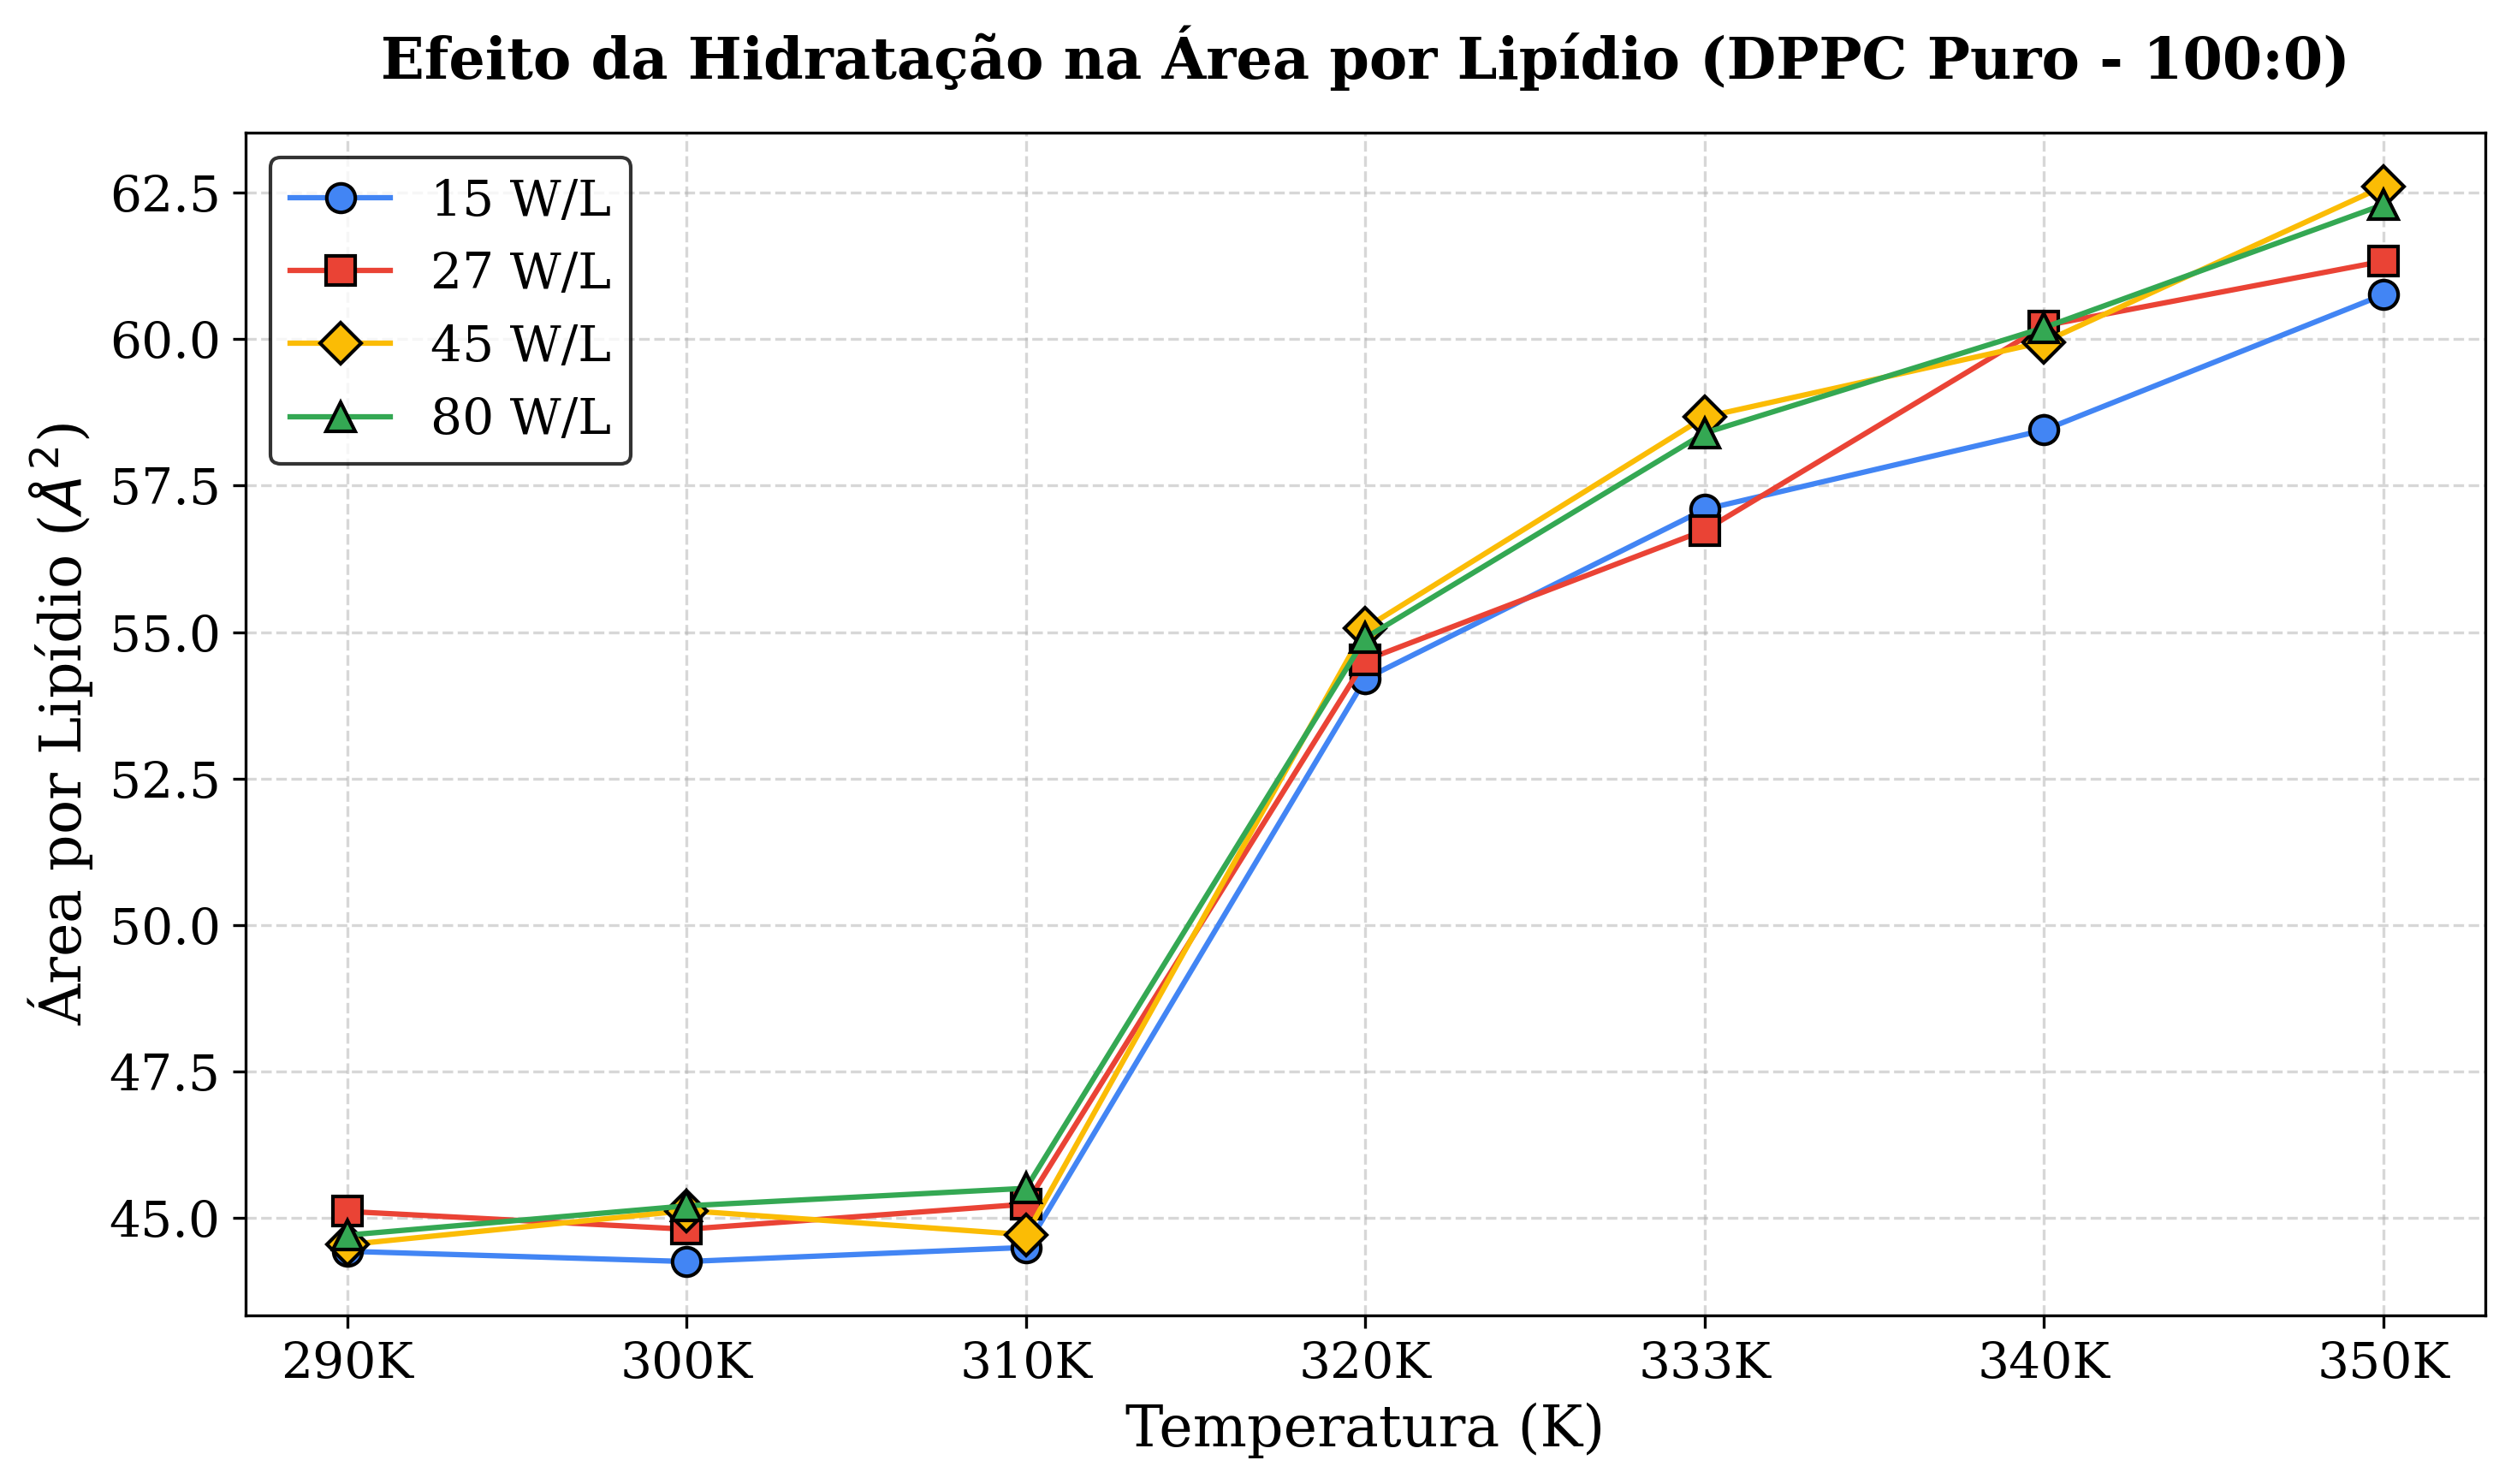
\includegraphics[width=\textwidth]{imagens/figura_4_1_google.png}
    \caption{Efeito global do gradiente de hidratação na expansão térmica lateral do DPPC puro (100:0). A convergência entre os regimes de 45 W/L e 80 W/L estabelece o limite termodinâmico de dilatação induzida por solvente para o modelo Martini 3.}
    \label{fig:comparativo_hidratacao}
\end{figure}

A Figura \ref{fig:mosaico_4_2} reforça este panorama ao ilustrar a dinâmica de transição termotrópica para os lipídios puros (DPPC e DSPC), evidenciando os primeiros sinais de retenção cinética em regimes de média e alta hidratação. Contudo, a modelagem \textit{coarse-grained} (CG) baseada no campo de força Martini 3 envolve compromissos termodinâmicos. Para garantir a reprodução precisa do comportamento cooperativo em misturas, o modelo impõe uma compactação artificial que subestima ligeiramente a $A_L$ na fase gel ($L_{\beta}$) e superestima a temperatura da transição principal ($T_m$) em aproximadamente 5 a 10 K \cite{pedersen2024}. 

% --- Figura 4.2: Mosaico DPPC vs DSPC ---
\begin{figure}[htpb]
    \centering
    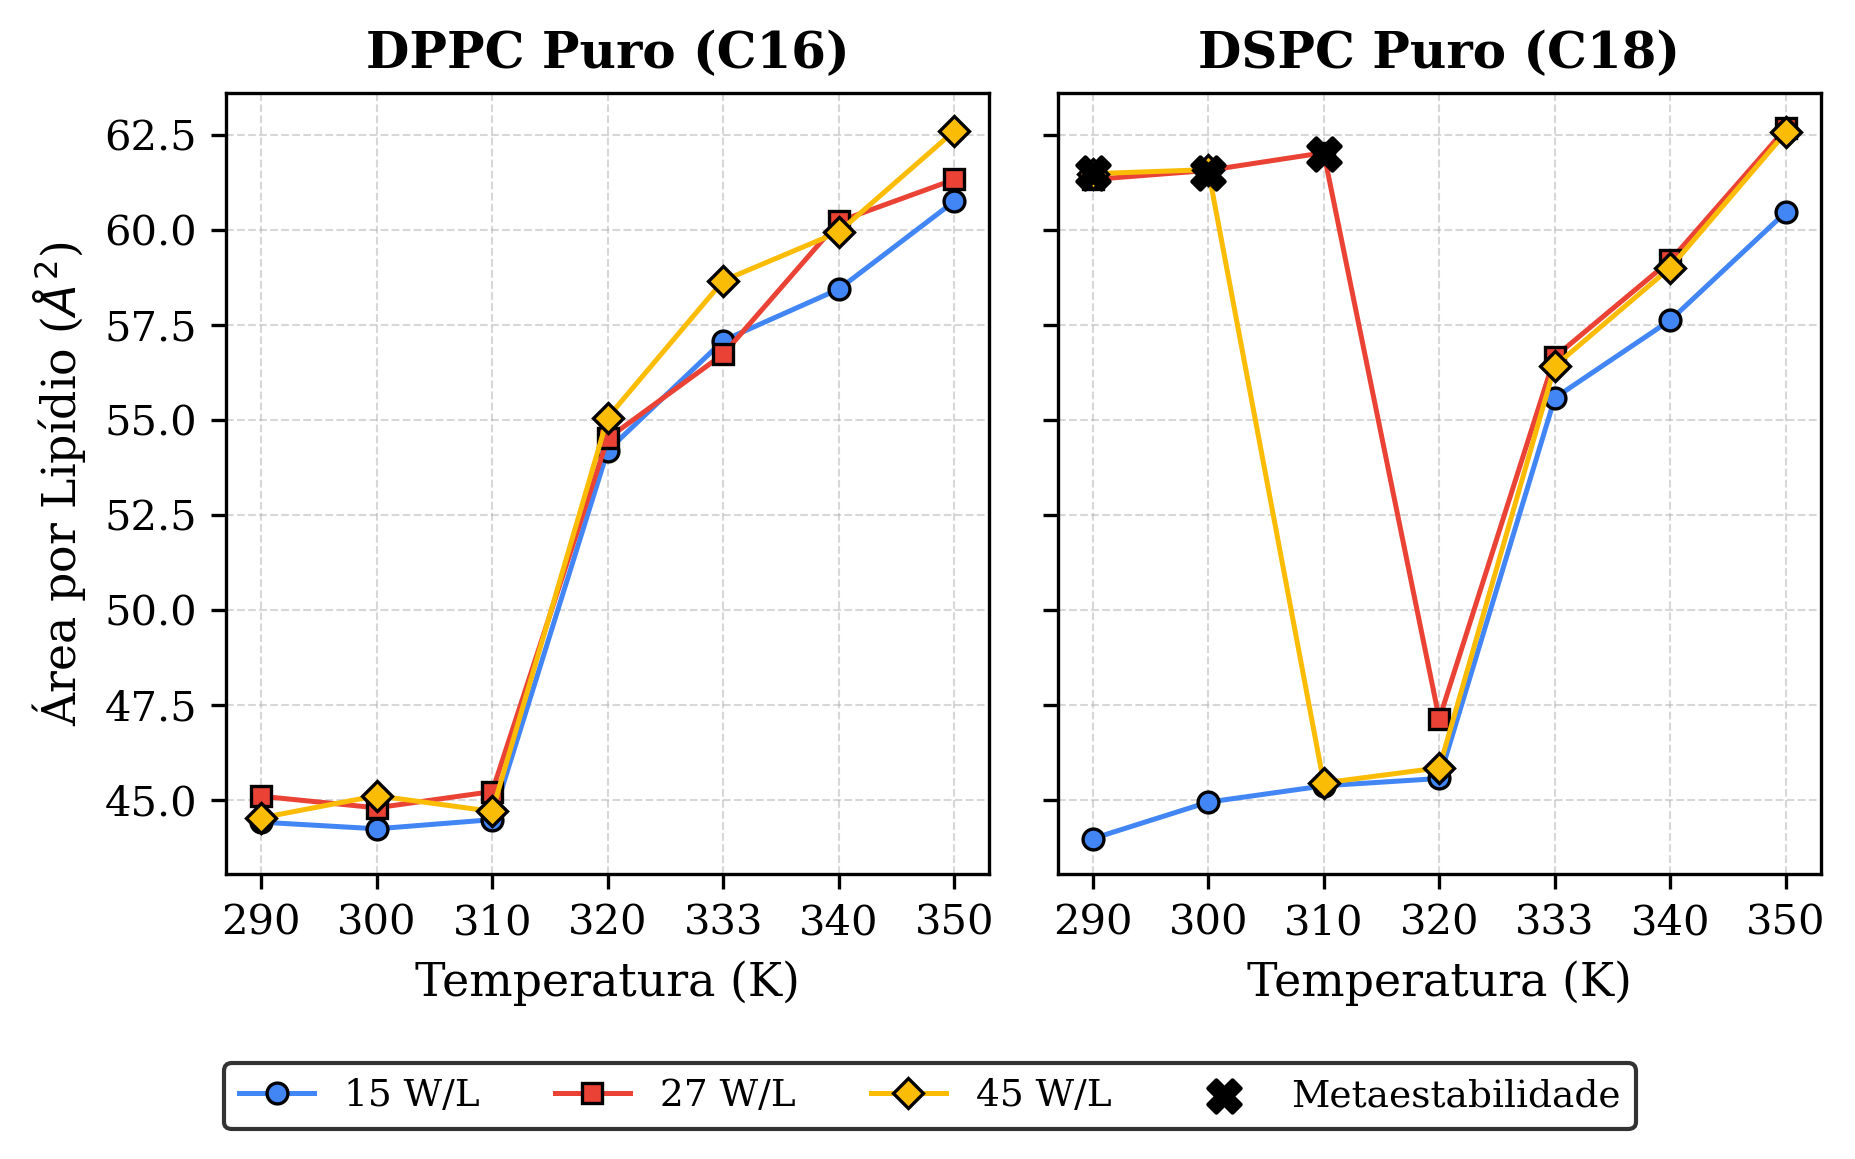
\includegraphics[width=\textwidth]{imagens/mosaico_figura_4_2.png}
    \caption{Influência da hidratação na transição termotrópica dos lipídios puros. À esquerda, a expansão do DPPC ($C_{16}$); à direita, a inércia do DSPC ($C_{18}$), evidenciando a armadilha cinética e a retenção em estados metaestáveis (marcadores X) sob média e alta hidratação.}
    \label{fig:mosaico_4_2}
\end{figure}

Devido a estes desvios térmicos intrínsecos, uma comparação isotérmica direta (temperatura por temperatura) entre as simulações e os dados experimentais mascararia o verdadeiro estado físico da membrana. Para evidenciar o deslocamento da temperatura de transição ($T_m$) e a severidade da metaestabilidade provocada pelo modelo Martini 3, a Tabela \ref{tab:comparativo_fases} confronta os estados experimentais de referência com toda a varredura térmica simulada para o sistema de alta hidratação (45W\_L).

\begin{table}[htpb]
    \centering
    \caption{Comparativo detalhado da evolução da Área por Lipídio ($A_L$) em função da temperatura, evidenciando o deslocamento da transição de fase no modelo Martini 3 (sistema 45W\_L).}
    \label{tab:comparativo_fases}
    \renewcommand{\arraystretch}{1.2}
    \resizebox{\textwidth}{!}{%
    \begin{tabular}{llcccl}
        \toprule
        \multirow{2}{*}{\textbf{Lipídio}} & \multicolumn{2}{c}{\textbf{Referência Experimental \cite{kucerka2011}}} & \multicolumn{3}{c}{\textbf{Simulação Martini 3 (Este Trabalho)}} \\
        \cmidrule(lr){2-3} \cmidrule(lr){4-6}
         & \textbf{Fase a Temp. (K)} & \textbf{$A_L$ (\AA$^2$)} & \textbf{Temp. (K)} & \textbf{$A_L$ (\AA$^2$)} & \textbf{Fase Observada} \\
        \midrule
        \multirow{7}{*}{\textbf{DPPC}} & \multirow{3}{*}{Gel ($L_{\beta}$) a 293} & \multirow{3}{*}{$47,4 \pm 0,5$}
         & 290 & $\sim 44,5$ & Gel ($L_{\beta}$) \\
         & & & 300 & $\sim 45,0$ & Gel ($L_{\beta}$) \\
         & & & 310 & $\sim 44,8$ & Gel ($L_{\beta}$) \\
        \cmidrule(lr){2-6}
         & \textit{Transição} ($T_m \approx 314$) & \textit{--} & 320 & $\sim 55,0$ & Transição de Fase \\
        \cmidrule(lr){2-6}
         & \multirow{3}{*}{Fluida ($L_{\alpha}$) a 323} & \multirow{3}{*}{$63,1 \pm 1,3$}
         & 333 & $\sim 58,6$ & Fluida ($L_{\alpha}$) \\
         & & & 340 & $\sim 60,0$ & Fluida ($L_{\alpha}$) \\
         & & & 350 & $\sim 62,6$ & Fluida ($L_{\alpha}$) \\
        \midrule
        \multirow{7}{*}{\textbf{DSPC}} & \multirow{4}{*}{Gel ($L_{\beta}$) a 293} & \multirow{4}{*}{$48,0 \pm 0,5$}
         & 290 & $\sim 61,5$ & Metaestável (Líq. Super-resf.) \\
         & & & 300 & $\sim 61,5$ & Metaestável (Líq. Super-resf.) \\
         & & & 310 & $\sim 45,5$ & Gel ($L_{\beta}$) \\
         & & & 320 & $\sim 45,8$ & Gel ($L_{\beta}$) \\
        \cmidrule(lr){2-6}
         & \textit{Transição} ($T_m \approx 328$) & \textit{--} & 333 & $\sim 56,5$ & Transição de Fase \\
        \cmidrule(lr){2-6}
         & \multirow{2}{*}{Fluida ($L_{\alpha}$) a 338} & \multirow{2}{*}{$65,5 \pm 1,3$}
         & 340 & $\sim 59,0$ & Fluida ($L_{\alpha}$) \\
         & & & 350 & $\sim 62,6$ & Fluida ($L_{\alpha}$) \\
        \bottomrule
    \end{tabular}%
    }
\end{table}

Na fase fluida ($L_{\alpha}$), as simulações a 350 K convergem para uma $A_L \approx 62,6$ \AA$^2$ tanto para o DPPC quanto para o DSPC. Estes valores encontram-se em rigorosa concordância com os perfis de espalhamento de raios-X e nêutrons, que reportam áreas de 63,1 \AA$^2$ e 65,5 \AA$^2$ para as respetivas fases fluidas \cite{kucerka2011}. O deslocamento térmico torna-se evidente ao observar-se que o DPPC simulado necessita atingir 350 K para igualar a dilatação que o lipídio real atinge a 323 K. No regime de gel ($L_{\beta}$), as simulações estabilizam em torno de 45,0 \AA$^2$, refletindo a compactação artificial do campo de força e justificando a ampla janela de transição térmica ($> 30$ K de diferença em relação à $T_m$ experimental).


A histerese térmica imposta pelo modelo \cite{pedersen2024} reflete-se de forma aguda na inércia termodinâmica do sistema de DSPC puro, evidenciada pela série temporal da Figura \ref{fig:estabilidade}. A 290 K e 300 K, a membrana falha em nucleiar espontaneamente, permanecendo retida num estado metaestável de líquido super-resfriado. Esta armadilha cinética é consequência do limite de resolução do mapeamento CG, que agrupa múltiplos átomos em esferas interativas, suprimindo flutuações \textit{trans-gauche} de caráter microscópico \cite{pedersen2024}. A divergência de nucleação entre o DPPC (que cristaliza prontamente) e o DSPC valida a alta sensibilidade estérica do modelo. Para discriminar caudas lipídicas com diferença de apenas dois carbonos, o DPPC utiliza contas de menor raio (\textit{small beads}), minimizando o volume colisional. Em contrapartida, as caudas do DSPC são mapeadas com contas regulares \cite{pedersen2024}. O maior raio destas exacerba a fricção estérica, fazendo com que as flutuações térmicas ($k_B T$) sejam insuficientes para contornar a alta penalidade entálpica de dessolvatação interfacial, aprisionando a membrana.

% --- Figura 4.4: Estabilidade / Série Temporal ---
\begin{figure}[htpb]
    \centering
    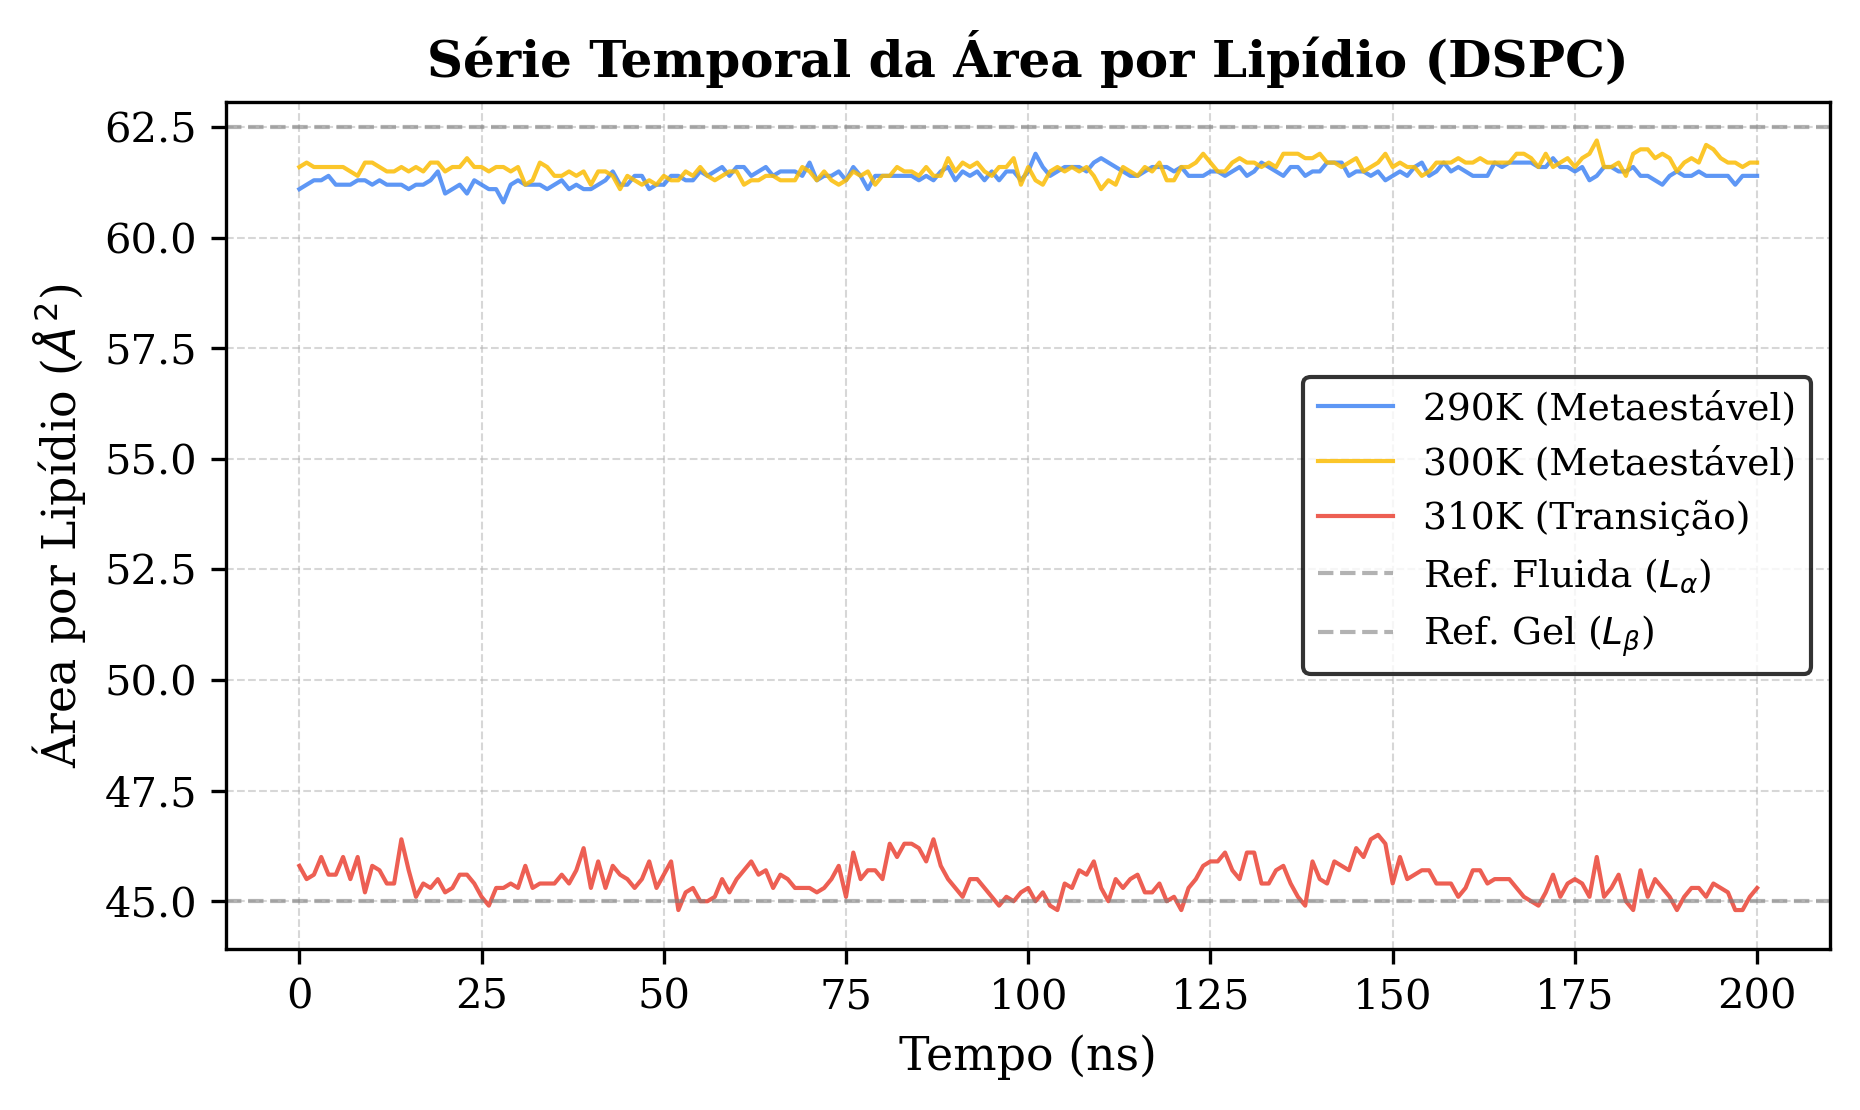
\includegraphics[width=\textwidth]{imagens/analise_estabilidade_DSPC_completa.png}
    \caption{Série temporal evidenciando a barreira de nucleação no DSPC puro (45W\_L). As trajetórias a 290 K e 300 K demonstram inércia cinética, falhando em transicionar espontaneamente para a fase gel ($L_{\beta}$) ao longo de 200 ns de simulação.}
    \label{fig:estabilidade}
\end{figure}

A restrição hídrica altera fundamentalmente esta paisagem de energia livre. No sistema de baixa hidratação (15W\_L, Figura \ref{fig:apl_15w}), a diminuição do volume livre e da blindagem dielétrica elimina a barreira de repulsão hídrica. Isso suprime a persistência dos estados super-resfriados, induzindo uma transição de fase cooperativa nítida mesmo para o DSPC. O regime intermediário (27W\_L, Figura \ref{fig:apl_27w}) atua como uma transição mecânica, onde a membrana ainda inicia retida em metaestabilidade, mas exibe uma cristalização tardia a 320 K.

% --- Figura 4.5: APL Baixa Hidratação (15W\_L) ---
\begin{figure}[htpb]
    \centering
    \includegraphics[width=\textwidth]{imagens/grafico_APL_15W\_L.png}
    \caption{Área por lipídio sob forte restrição hídrica (15W\_L). A diminuição da blindagem dielétrica e do volume livre de solvente suprime os estados metaestáveis, induzindo uma transição de fase cooperativa em toda a matriz binária.}
    \label{fig:apl_15w}
\end{figure}

% --- Figura 4.6: APL Média Hidratação (27W\_L) ---
\begin{figure}[htpb]
    \centering
    \includegraphics[width=\textwidth]{imagens/grafico_APL_27W\_L.png}
    \caption{Área por lipídio sob hidratação intermediária (27W\_L). O sistema atua como um regime mecânico de transição, onde a matriz de DSPC inicia retida na fase fluida a 290 K, mas cede a uma cristalização tardia a 320 K.}
    \label{fig:apl_27w}
\end{figure}

A heterogeneidade molecular em sistemas biológicos atua como um contorno para estas barreiras termodinâmicas. A Figura \ref{fig:mosaico_misturas} consolida este comportamento através do mosaico global das misturas binárias. Diferente dos sistemas puros, as misturas apresentam zonas de coexistência onde a inclusão de cadeias mais curtas ($C_{16}$, DPPC) nas matrizes de DSPC atua como um facilitador cinético, reduzindo a energia de ativação necessária para o empacotamento apolar e restaurando a cooperatividade da transição.

% --- Figura 4.7: Mosaico Global das Misturas ---
\begin{figure}[htpb]
    \centering
    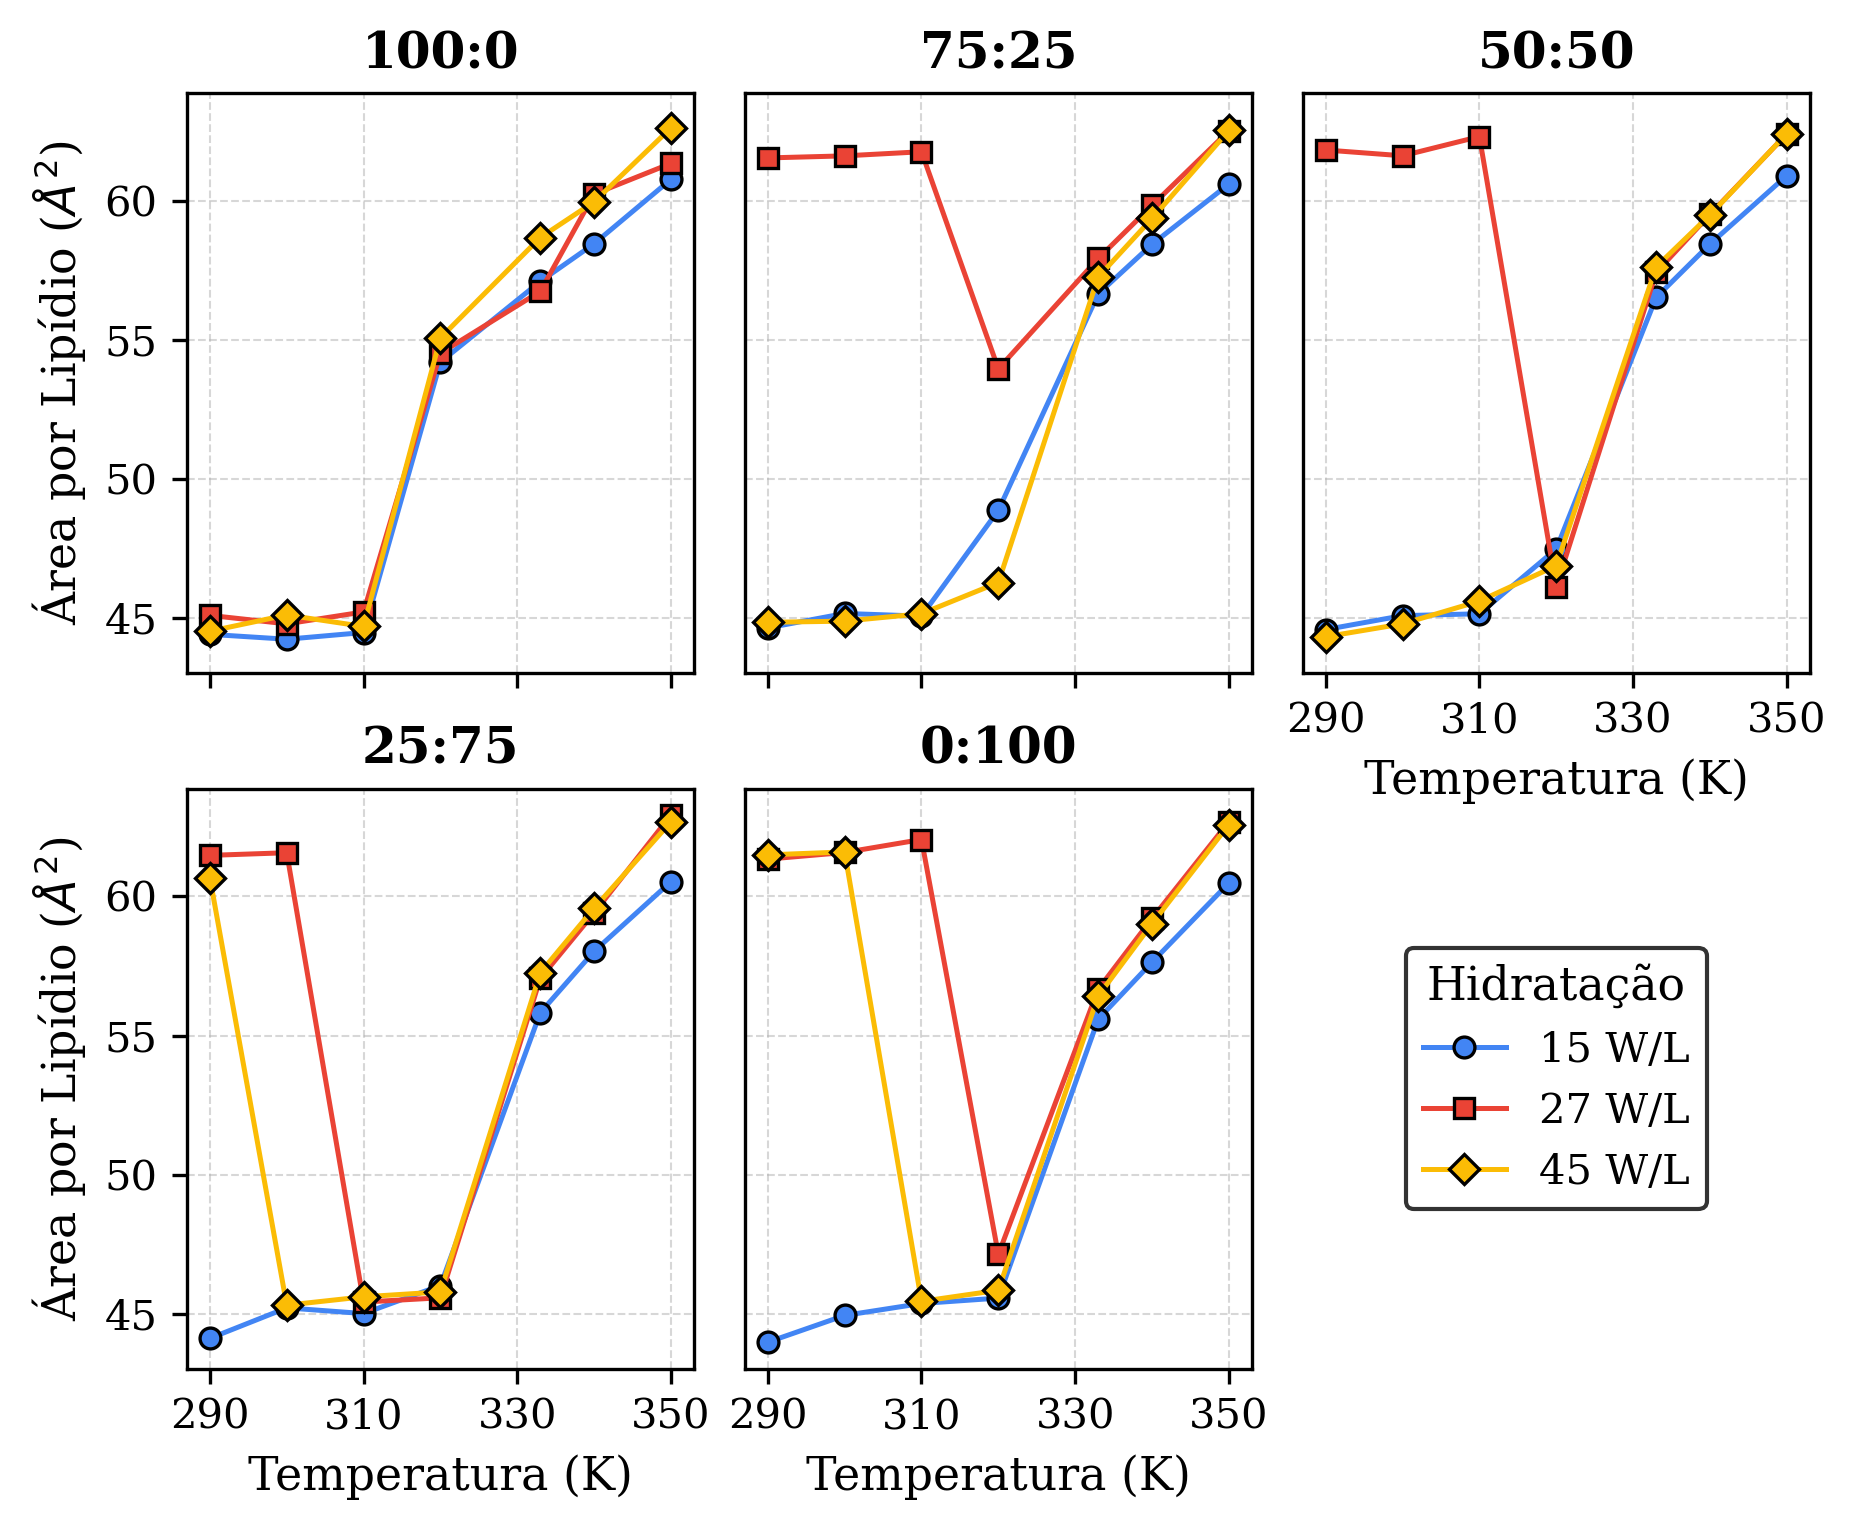
\includegraphics[width=\textwidth]{imagens/comparativo_global_misturas.png}
    \caption{Mosaico global da expansão térmica para as misturas binárias sob três diferentes regimes hídricos. Observa-se que a inclusão de DPPC ($C_{16}$) nas matrizes ricas em DSPC atua como facilitador cinético, restaurando a transição de fase nas hidratações mais altas.}
    \label{fig:mosaico_misturas}
\end{figure}

% --- INSIRA O SEU TEXTO ORIGINAL SOBRE A ESPESSURA (FIGURA 4.8) A PARTIR DESTE PONTO ---


\subsubsection*{Espessura da Bicamada e Efeito do Comprimento da Cadeia}

Para complementar a análise termodinâmica da área por lipídio, a espessura da membrana (distância transversal média entre os grupos polares, $D_B$) foi investigada em função da temperatura para o sistema de alta hidratação (45W\_L). Como ilustrado na Figura \ref{fig:espessura_45W\_L}, a secção transversal da bicamada apresenta uma rigorosa correlação inversamente proporcional à sua expansão lateral.

% --- Figura: Espessura da Membrana (A imagem que havia sumido) ---
\begin{figure}[htpb]
    \centering
    % Substitua o nome do arquivo abaixo pelo nome exato da sua imagem de espessura!
    \includegraphics[width=0.85\textwidth]{imagens/grafico_espessura_45W\_L.png}
    \caption{Evolução termotrópica da Espessura da Bicamada ($D_B$) sob alta hidratação (45 W/L). A expansão térmica lateral exige, por conservação de volume, a contração transversal do núcleo hidrofóbico. Nota-se o claro gradiente de espessura ditado pelo comprimento das caudas ($C_{16}$ vs. $C_{18}$).}
    \label{fig:espessura_45W\_L}
\end{figure}

Na fase gel ($T < 310$ K), as cadeias acílicas encontram-se altamente ordenadas e estendidas na conformação \textit{all-trans}, resultando em espessuras máximas que atingem aproximadamente $4,6$ nm para a matriz de DPPC e $5,0$ nm para o DSPC. O incremento térmico e a transição para a fase fluida ($L_\alpha$) elevam exponencialmente a probabilidade de isomerizações rotacionais \textit{trans-gauche}, induzindo profunda desordem nas cadeias hidrocarbônicas \cite{kucerka2011}. Mecanicamente, esta desordem térmica exige a dilatação lateral da estrutura e a sua consequente contração transversal, evidenciada pela queda abrupta nas curvas termotrópicas \cite{kucerka2011}.


Este comportamento e a dependência em relação ao comprimento da cadeia espelham com precisão as tendências estruturais reportadas em ensaios de espalhamento de raios-X e nêutrons \cite{kucerka2011}. Na fase fluida, a espessura total ($D_B$) é sistematicamente superior para lipídios de cadeia estendida. Termodinamicamente, o incremento das interações atrativas de dispersão de van der Waals nas caudas maiores atua como um contrapeso entálpico, mitigando parcialmente o colapso transversal induzido pela desordem térmica \cite{kucerka2011}.

Assim como observado na dinâmica de dilatação lateral, a comparação isotérmica direta mascararia o deslocamento térmico inerente à modelagem \textit{coarse-grained}. Para avaliar a precisão estrutural do mapeamento ao longo das diferentes fases físicas, a Tabela \ref{tab:comparativo_espessura} alinha a varredura térmica completa da espessura simulada com os referenciais experimentais correspondentes.

\begin{table}[htpb]
    \centering
    \caption{Comparativo detalhado da evolução da Espessura da Bicamada ($D_B$) em função da temperatura, evidenciando a correlação termomecânica no modelo Martini 3 (sistema 45W\_L).}
    \label{tab:comparativo_espessura}
    \renewcommand{\arraystretch}{1.2}
    \resizebox{\textwidth}{!}{%
    \begin{tabular}{llcccl}
        \toprule
        \multirow{2}{*}{\textbf{Lipídio}} & \multicolumn{2}{c}{\textbf{Referência Experimental \cite{kucerka2011}}} & \multicolumn{3}{c}{\textbf{Simulação Martini 3 (Este Trabalho)}} \\
        \cmidrule(lr){2-3} \cmidrule(lr){4-6}
         & \textbf{Fase a Temp. (K)} & \textbf{Espessura (nm)} & \textbf{Temp. (K)} & \textbf{Espessura (nm)} & \textbf{Fase Observada} \\
        \midrule
        \multirow{7}{*}{\textbf{DPPC}} & \multirow{3}{*}{Gel ($L_{\beta}$)} & \multirow{3}{*}{--}
         & 290 & $\sim 4,62$ & Gel ($L_{\beta}$) \\
         & & & 300 & $\sim 4,62$ & Gel ($L_{\beta}$) \\
         & & & 310 & $\sim 4,62$ & Gel ($L_{\beta}$) \\
        \cmidrule(lr){2-6}
         & \multirow{2}{*}{Fluida ($L_{\alpha}$) a 323} & \multirow{2}{*}{$3,90 \pm 0,08$} & 320 & $\sim 4,16$ & Transição de Fase \\
         & & & 333 & $\sim 4,01$ & Fluida ($L_{\alpha}$) \\
        \cmidrule(lr){2-6}
         & \multirow{2}{*}{Fluida ($L_{\alpha}$) a 333} & \multirow{2}{*}{$3,81 \pm 0,08$}
         & 340 & $\sim 3,97$ & Fluida ($L_{\alpha}$) \\
         & & & 350 & $\sim 3,85$ & Fluida ($L_{\alpha}$) \\
        \midrule
        \multirow{7}{*}{\textbf{DSPC}} & \multirow{4}{*}{Gel ($L_{\beta}$)} & \multirow{4}{*}{--}
         & 290 & $\sim 4,15$ & Metaestável (Líq. Super-resf.) \\
         & & & 300 & $\sim 4,20$ & Metaestável (Líq. Super-resf.) \\
         & & & 310 & $\sim 4,98$ & Gel ($L_{\beta}$) \\
         & & & 320 & $\sim 5,00$ & Gel ($L_{\beta}$) \\
        \cmidrule(lr){2-6}
         & \textit{Transição} ($T_m \approx 328$) & \textit{--} & 333 & $\sim 4,53$ & Transição de Fase \\
        \cmidrule(lr){2-6}
         & \multirow{2}{*}{Fluida ($L_{\alpha}$) a 338} & \multirow{2}{*}{$4,22 \pm 0,08$}
         & 340 & $\sim 4,40$ & Fluida ($L_{\alpha}$) \\
         & & & 350 & $\sim 4,25$ & Fluida ($L_{\alpha}$) \\
        \bottomrule
    \end{tabular}%
    }
\end{table}

A análise quantitativa revela a precisão estrutural da simplificação molecular. A literatura estabelece espessuras experimentais de $3,90$ nm para o DPPC (a 323 K) e $4,22$ nm para o DSPC (a 333 K) \cite{kucerka2011}. No limite superior do regime totalmente fluido simulado (350 K), a secção transversal converge para $\sim 3,85$ nm no sistema homólogo de DPPC, enquanto o DSPC estabiliza-se em $\sim 4,25$ nm. A estrita preservação deste gradiente estrutural ($\Delta \approx 0,2$ nm) entre os domínios $C_{16}$ e $C_{18}$ valida a capacidade da discretização topológica em reproduzir a mecânica fina do empacotamento hidrofóbico.

Adicionalmente, nota-se a ausência de anomalias evidentes (\textit{outliers}) na comparação dos dados obtidos ao longo da progressão térmica \cite{pedersen2024}. Este comportamento atesta que a dependência térmica das propriedades geométricas da bicamada lipídica é reproduzida de maneira fisicamente coerente: a elevação da temperatura conduz invariavelmente ao incremento da Área por Lipídio e à respectiva diminuição da espessura da bicamada na fase líquida. Esta estabilidade fenomenológica consolida a tese de que os parâmetros de ligação (\textit{bonded parameters}) calibrados no modelo operam de forma preditiva e são rigorosamente válidos através de uma ampla gama de temperaturas biologicamente relevantes \cite{pedersen2024}.

Por fim, o atraso cinético revelado na dinâmica lateral também assina a secção transversal do DSPC. Nas temperaturas em que a membrana permaneceu aprisionada em metaestabilidade (290 K e 300 K), a espessura exibiu uma contração anômala (na faixa de $4,15$ a $4,20$ nm), comprovando que a presença da água de hidratação aprisionada nos interstícios polares inviabilizou o estiramento vertical pleno das caudas apolares. O salto abrupto para a casa dos $5,00$ nm, deflagrado estritamente aos 310 K, sinaliza a expulsão desta água interfacial e atua como a resposta morfológica definitiva da cristalização mecânica para a fase gel autêntica ($L_{\beta}$).

\subsection{Modulação Eletrostática e o Efeito Condensador do Colesterol}

A introdução de colesterol na matriz lipídica altera fundamentalmente a termodinâmica da bicamada. Para isolar o efeito estrutural do esterol, avaliou-se inicialmente o sistema sob alta hidratação (40 W/L) na ausência de íons explícitos. O mosaico global da expansão térmica (Figura \ref{fig:mosaico_chol_global}) evidencia o impacto de concentrações crescentes de colesterol (0\%, 3\% e 30\% em mol) sobre as misturas binárias de DPPC e DSPC.

% --- Figura 4.8: Mosaico Global do Colesterol (Sem Íons) ---
\begin{figure}[htpb]
    \centering
    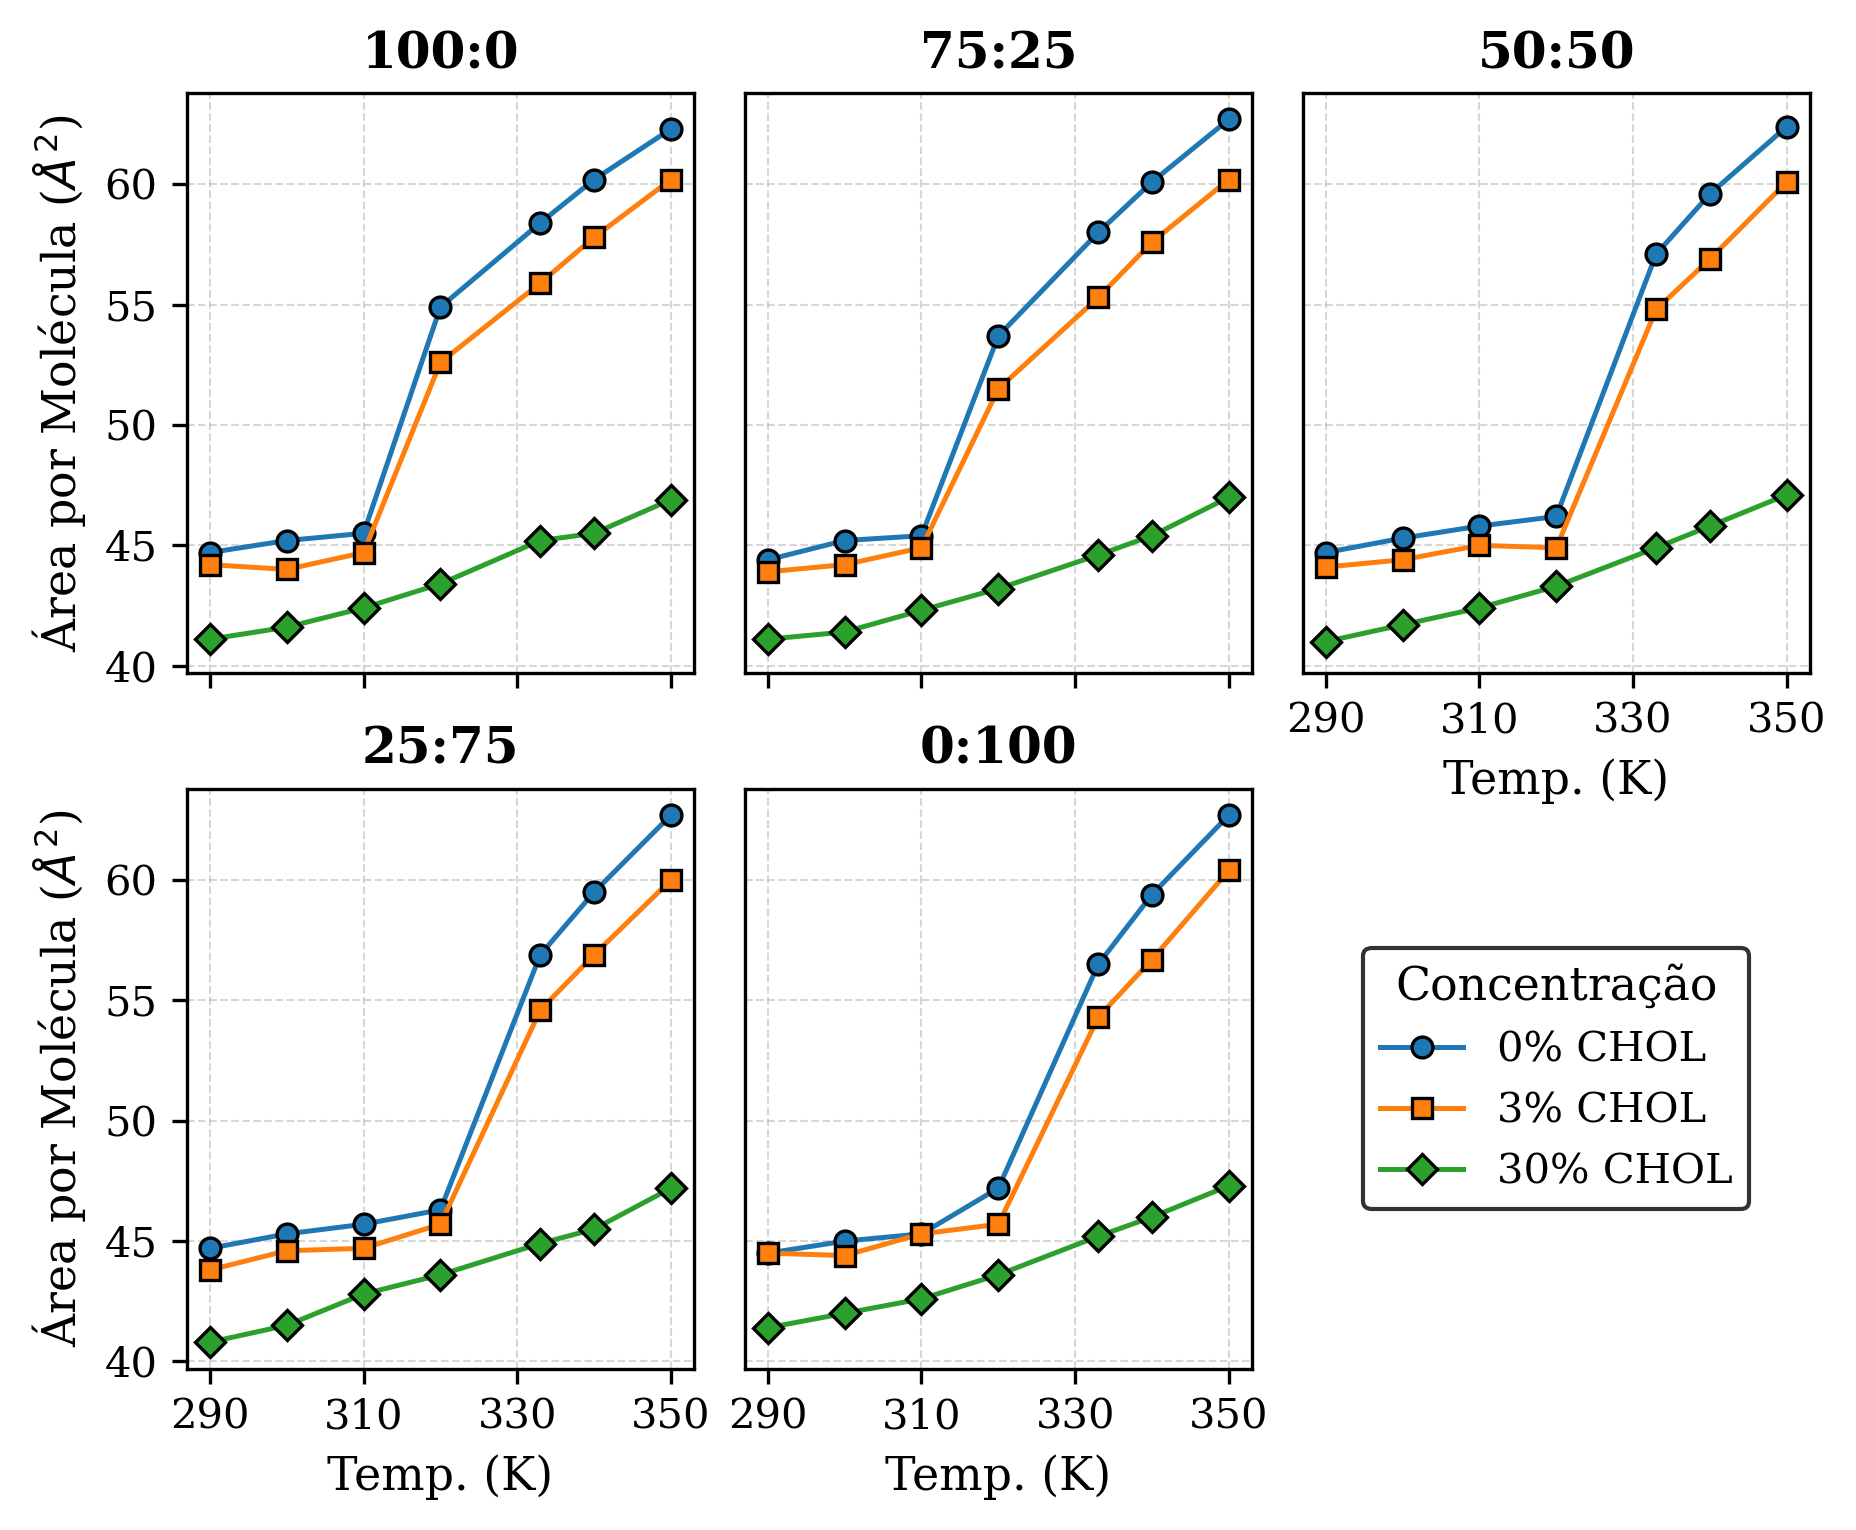
\includegraphics[width=\textwidth]{imagens/comparativo_chol_global.png}
    \caption{Mosaico da expansão térmica para misturas binárias de DPPC/DSPC sob diferentes concentrações de colesterol (0\%, 3\% e 30\% em mol). Observa-se a supressão progressiva da transição de fase cooperativa em função do aumento da saturação por esterol.}
    \label{fig:mosaico_chol_global}
\end{figure}

A análise revela que a área por molécula apresenta um decaimento não-linear, de caráter exponencial, à medida que a concentração de colesterol aumenta \cite{kheyfets2015}. % Este comportamento macroscópico é perfeitamente fundamentado pela mecânica estatística através do modelo de cordas flexíveis (\textit{flexible strings model}) \cite{kheyfets2015}. % Sob esta ótica, os fosfolipídios atuam como cordas flexíveis sujeitas a flutuações térmicas, enquanto a molécula de colesterol atua mecanicamente como uma haste rígida (\textit{rigid rod}) de rigidez infinita \cite{kheyfets2015}. % A presença do esterol suprime os graus de liberdade vibracionais das cadeias acílicas adjacentes, forçando o estiramento das mesmas e induzindo o achatamento exponencial da área lateral \cite{kheyfets2015}. %

No regime de baixa concentração (3\%), o colesterol atua como uma impureza que perturba o empacotamento da fase gel, mas preserva a transição de primeira ordem para a fase fluida ($L_{\alpha}$). Em contrapartida, sob alta saturação (30\%), o efeito condensador torna-se absoluto. Para examinar a mecânica detalhada desta fase líquida-ordenada ($L_o$), a Figura \ref{fig:apl_chol_30} isola o perfil termotrópico do sistema com 30\% de esterol.

% --- Figura 4.9: Colesterol 30% (Efeito Condensador Linear) ---
\begin{figure}[htpb]
    \centering
    \includegraphics[width=\textwidth]{imagens/grafico_APL_CHOL\_30.png}
    \caption{Área média por molécula para o sistema com 30\% de colesterol. O efeito condensador lineariza a expansão térmica e anula a influência do comprimento da cadeia acílica, resultando na convergência das curvas para as diferentes misturas de DPPC/DSPC.}
    \label{fig:apl_chol_30}
\end{figure}

Neste regime, a expansão térmica torna-se estritamente linear. A restrição imposta pela "haste rígida" do colesterol é tão dominante que suprime a transição de fase e sobrepõe-se à influência do comprimento da cadeia hidrocarbônica \cite{kheyfets2015}. % Isto resulta numa notável convergência das curvas de expansão para todas as misturas de DPPC e DSPC, demonstrando que, em concentrações elevadas, as propriedades elásticas da membrana são governadas quase exclusivamente pelo esterol.

\subsubsection*{Efeito Combinado de Colesterol e Íons na Dinâmica Lateral}

As membranas biológicas reais operam imersas numa fase aquosa rica em eletrólitos, cuja presença dita interações interfaciais críticas. Para aproximar o modelo deste cenário fisiológico, introduziu-se 0,15 M de NaCl, promovendo a ancoragem eletrostática e a blindagem dielétrica nas cabeças polares. O impacto global desta adição, combinada a diferentes níveis de saturação de colesterol, encontra-se documentado na Figura \ref{fig:mosaico_salino}.

% --- Figura 4.10: Mosaico Global do Colesterol com SAL ---
\begin{figure}[htpb]
    \centering
    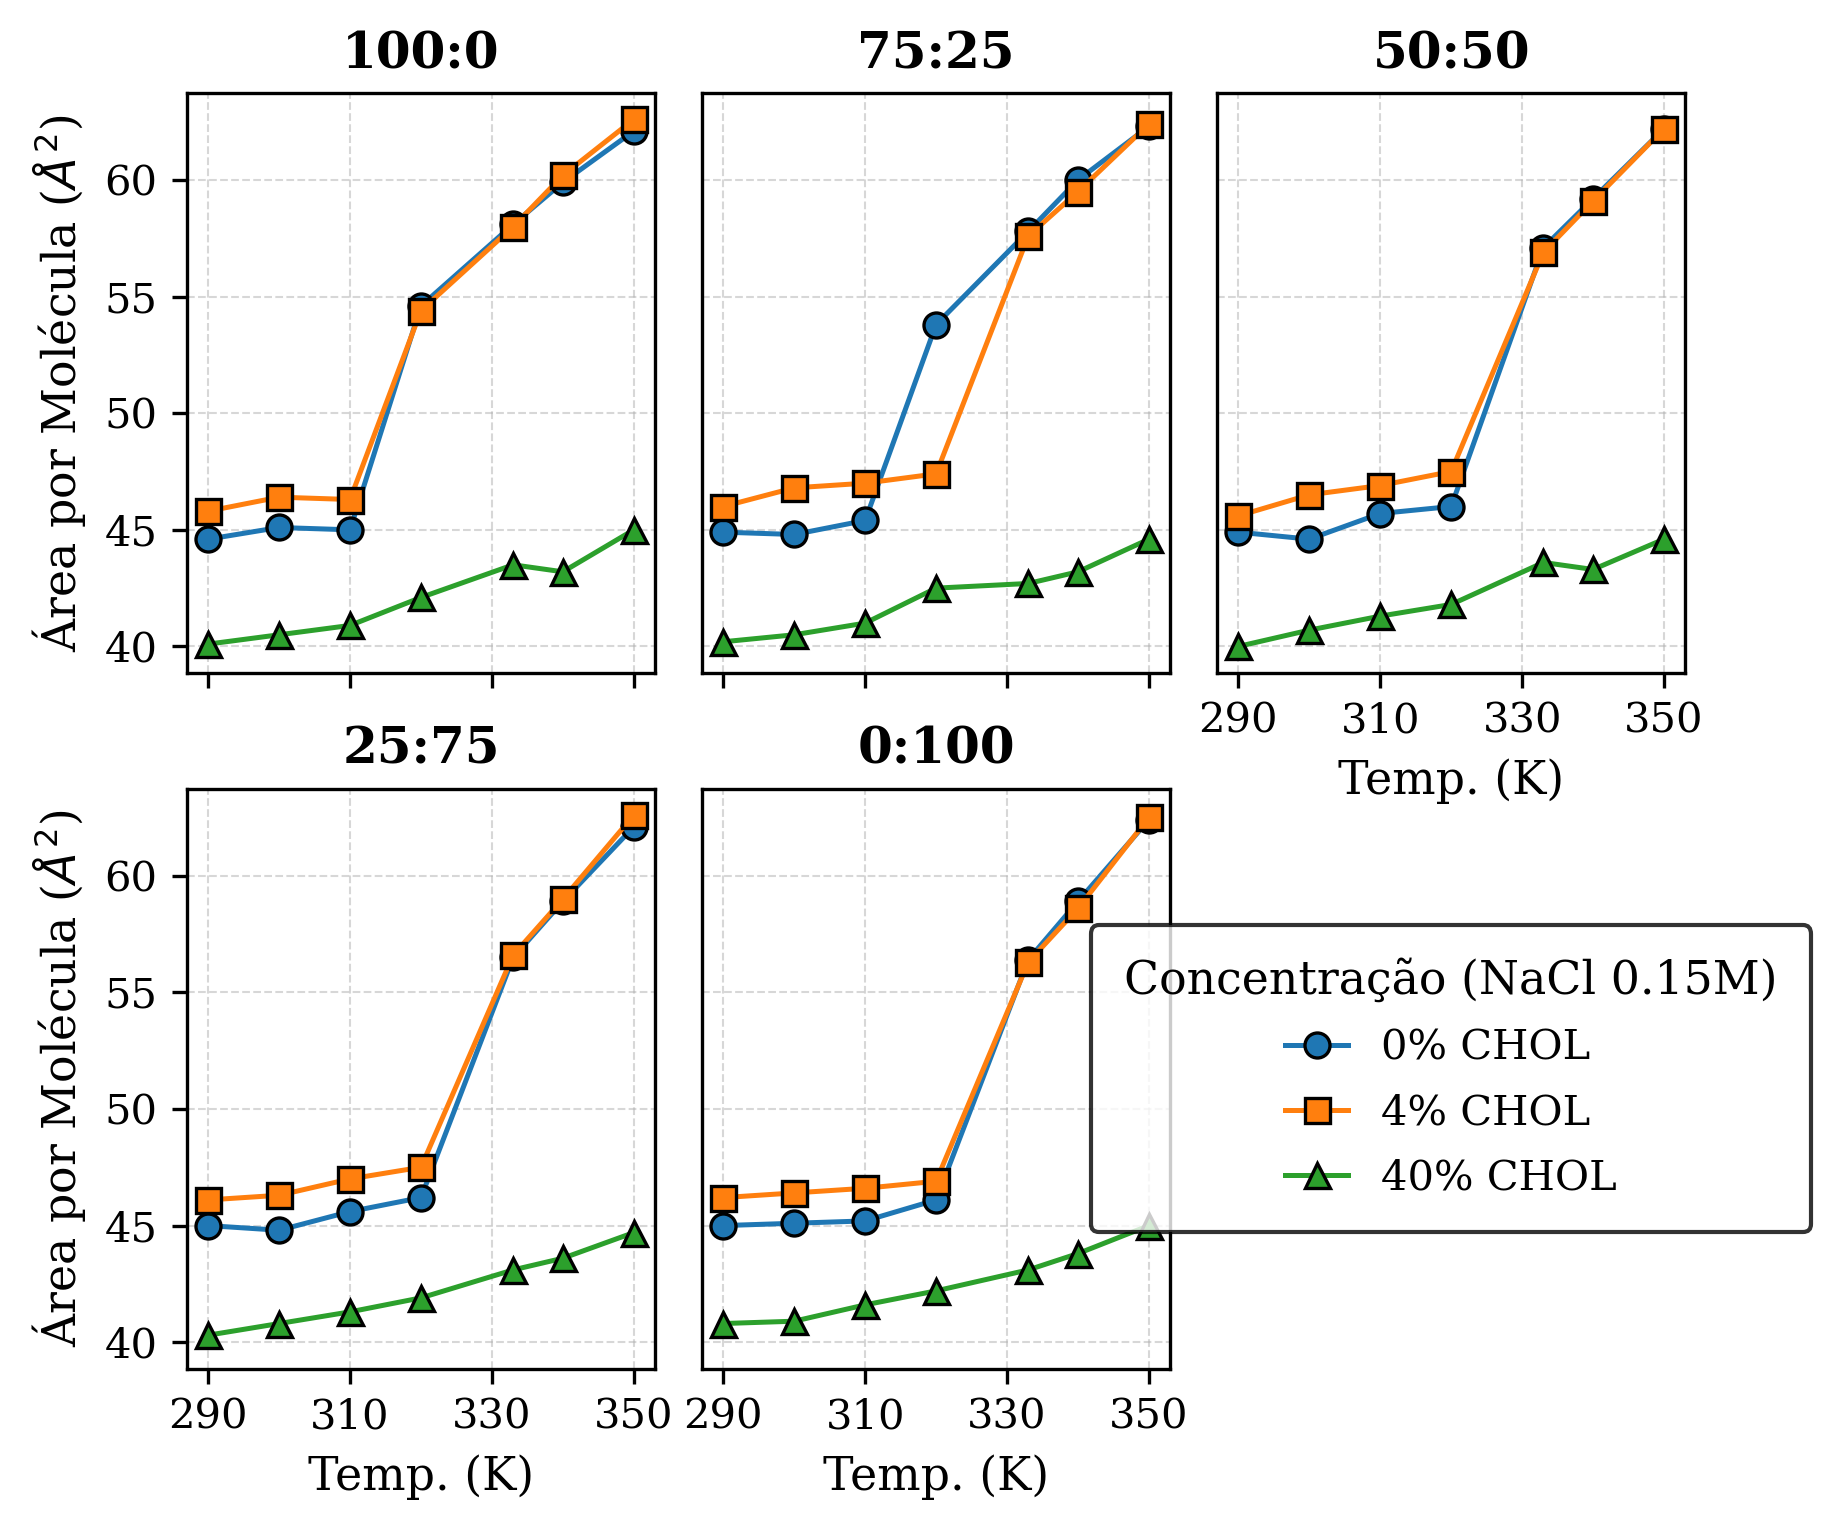
\includegraphics[width=\textwidth]{imagens/comparativo_global_salino.png}
    \caption{Mosaico termotrópico para as misturas binárias de DPPC/DSPC em meio salino fisiológico (0,15 M NaCl). Observa-se que a adição massiva de colesterol (40\% em mol) sobrepõe-se à coordenação iônica interfacial, anulando a cooperatividade em todas as proporções estequiométricas.}
    \label{fig:mosaico_salino}
\end{figure}

O comportamento do sistema revela uma delicada competição de forças. No sistema de controle puramente lipídico e com 4\% de colesterol, os íons exercem um papel estabilizador evidente: a coordenação dos cátions de sódio ($Na^+$) com os oxigênios carbonílicos favorece o empacotamento lateral, mantendo uma transição de fase de primeira ordem vigorosa a aproximadamente 320 K. 

No entanto, a inserção de 40\% de colesterol impõe uma retificação física incontornável. A dominância termomecânica do esterol induz a condensação severa das caudas flexíveis, achatando a curva termotrópica em todas as frações lipídicas (convergência para valores entre $43$ e $45$ \AA$^2$). Esta dinâmica demonstra que a rigidez imposta pela formação da fase $L_o$ anula a cooperatividade intrínseca da matriz lipídica, sobrepondo-se até mesmo à forte ancoragem elétrica proporcionada pela rede salina.

\vspace{1em}
\noindent\textbf{Influência da Força Iônica e Baixas Concentrações de Colesterol}

A análise da Figura \ref{fig:mosaico_salino} apresenta a evolução da APL para os sistemas em meio salino ($0,15$ M de NaCl). Observa-se que, para o sistema puro, a transição ocorre de forma acentuada entre 310 K e 333 K. 

Curiosamente, a inserção de 4\% de colesterol promove um comportamento dual, sugerindo que pequenas quantidades de esterol atuam como impurezas estruturais na fase gel \cite{pedersen2024}.

% =====================================================================
% SECÇÃO 4.3 - FUNDAMENTOS TERMODINÂMICOS
% =====================================================================

\subsection{Fundamentos Termodinâmicos: O Mecanismo de Compensação Isoperibólica}

\vspace{1em}
\noindent\textbf{Cálculo da Energia Total e Propagação de Incerteza (Tipo C)}

Para fundamentar empiricamente o balanço termodinâmico global da caixa de simulação, definiu-se a Energia Total ($E_{Tot}$) como o somatório algébrico das contribuições não-covalentes globais ($E_{Tot} = E_{Coulomb} + E_{LJ}$). 

Uma vez que as parcelas de Coulomb e de Lennard-Jones consistem em variáveis macroscópicas independentes derivadas das flutuações estatísticas intrínsecas ao campo de força (Incertezas do Tipo A), a incerteza combinada da Energia Total ($u_{Tot}$) exige um tratamento metrológico específico. De acordo com as diretrizes e normativas de Metrologia adotadas na literatura laboratorial \cite{ufgfisexp2020}, a propagação da incerteza para grandezas obtidas indiretamente enquadra-se metodologicamente como uma Incerteza do Tipo C. A sua magnitude final é determinada pelo cômputo da raiz quadrada da soma em quadratura das incertezas-padrão componentes:

\begin{equation}
    u_{Tot} = \sqrt{\left(\frac{\partial E_{Tot}}{\partial E_{Coulomb}} u_{Coulomb}\right)^2 + \left(\frac{\partial E_{Tot}}{\partial E_{LJ}} u_{LJ}\right)^2} = \sqrt{u_{Coulomb}^2 + u_{LJ}^2}
\end{equation}

Os resultados absolutos desta propagação metrológica para todos os patamares térmicos encontram-se tabulados de forma sistemática na Tabela \ref{tab:dados_brutos_energias} (Anexos). Com a exatidão quantitativa resguardada na íntegra, a presente secção foca-se na interpretação fenomenológica e qualitativa do comportamento matricial das membranas lipídicas.


\vspace{1em}
\noindent\textbf{Análise Termodinâmica Global: Coulomb vs. Lennard-Jones }

A análise comparativa das energias eletrostáticas (Coulomb, Figura \ref{fig:coulomb_comparativo}) e das forças de dispersão (Lennard-Jones, Figura \ref{fig:lj_comparativo}) permite distinguir os eixos termodinâmicos que governam a estabilidade da membrana. Os dados indicam que a interface polar e o núcleo apolar da bicamada respondem de forma distinta aos estresses térmicos e químicos.

Conforme evidenciado pela Figura \ref{fig:coulomb_comparativo}, as interações de Coulomb apresentam dependência acentuada da composição iônica do solvente e do grau de hidratação. Enquanto as membranas puras em meio sem sal exibem energias de Coulomb limitadas pelas interações entre os dipolos das cabeças zwitteriônicas, a adição de NaCl induz uma estabilização eletrostática expressiva. Este decréscimo energético decorre da coordenação específica de iões $Na^+$ com os grupos carbonílicos e fosfato das cabeças lipídicas \cite{bockmann2003, javanainen2017}, formando pontes eletrostáticas que conferem maior coesão à interface.

\begin{figure}[H]
    \centering
    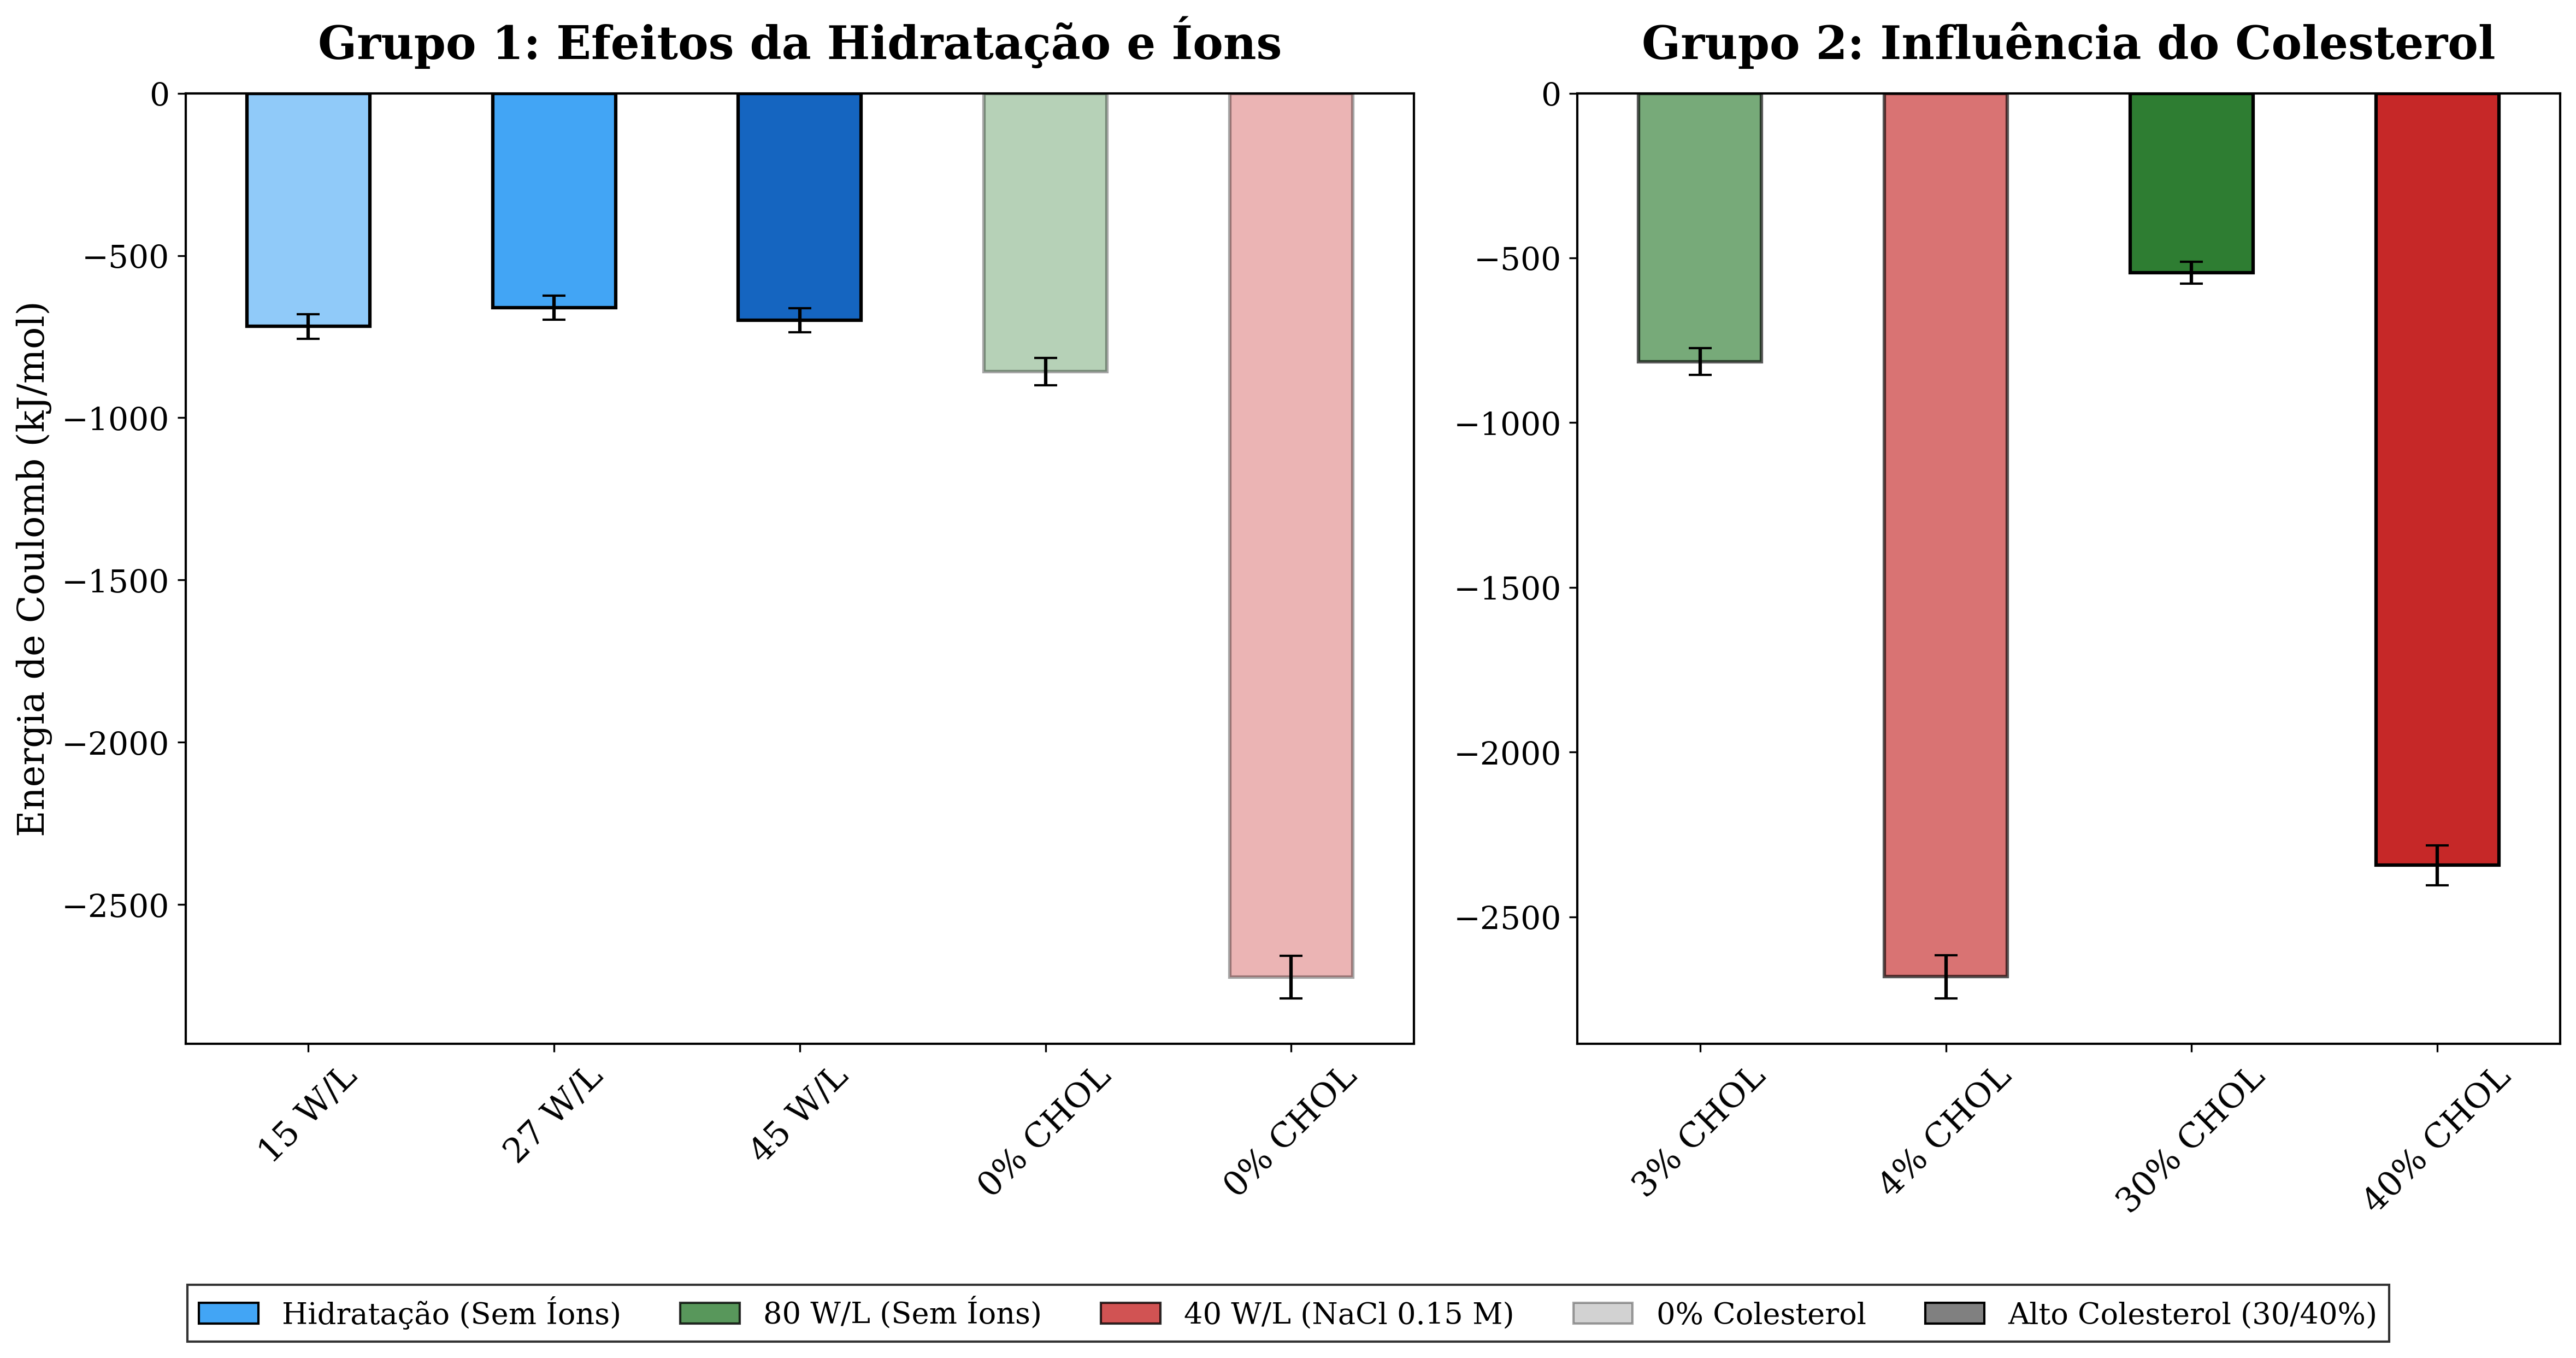
\includegraphics[width=0.9\textwidth]{imagens/comparativo_Coulomb_Exato.png}
    \caption{Energias eletrostáticas (Coulomb) médias. O Grupo 1 (controles) demonstra o impacto da hidratação, enquanto o sistema com NaCl (vermelho) evidencia a estabilização por coordenação iónica. No Grupo 2, o colesterol não altera significativamente o domínio eletrostático devido à sua neutralidade elétrica.}
    \label{fig:coulomb_comparativo}

    \vspace{0.8cm}

    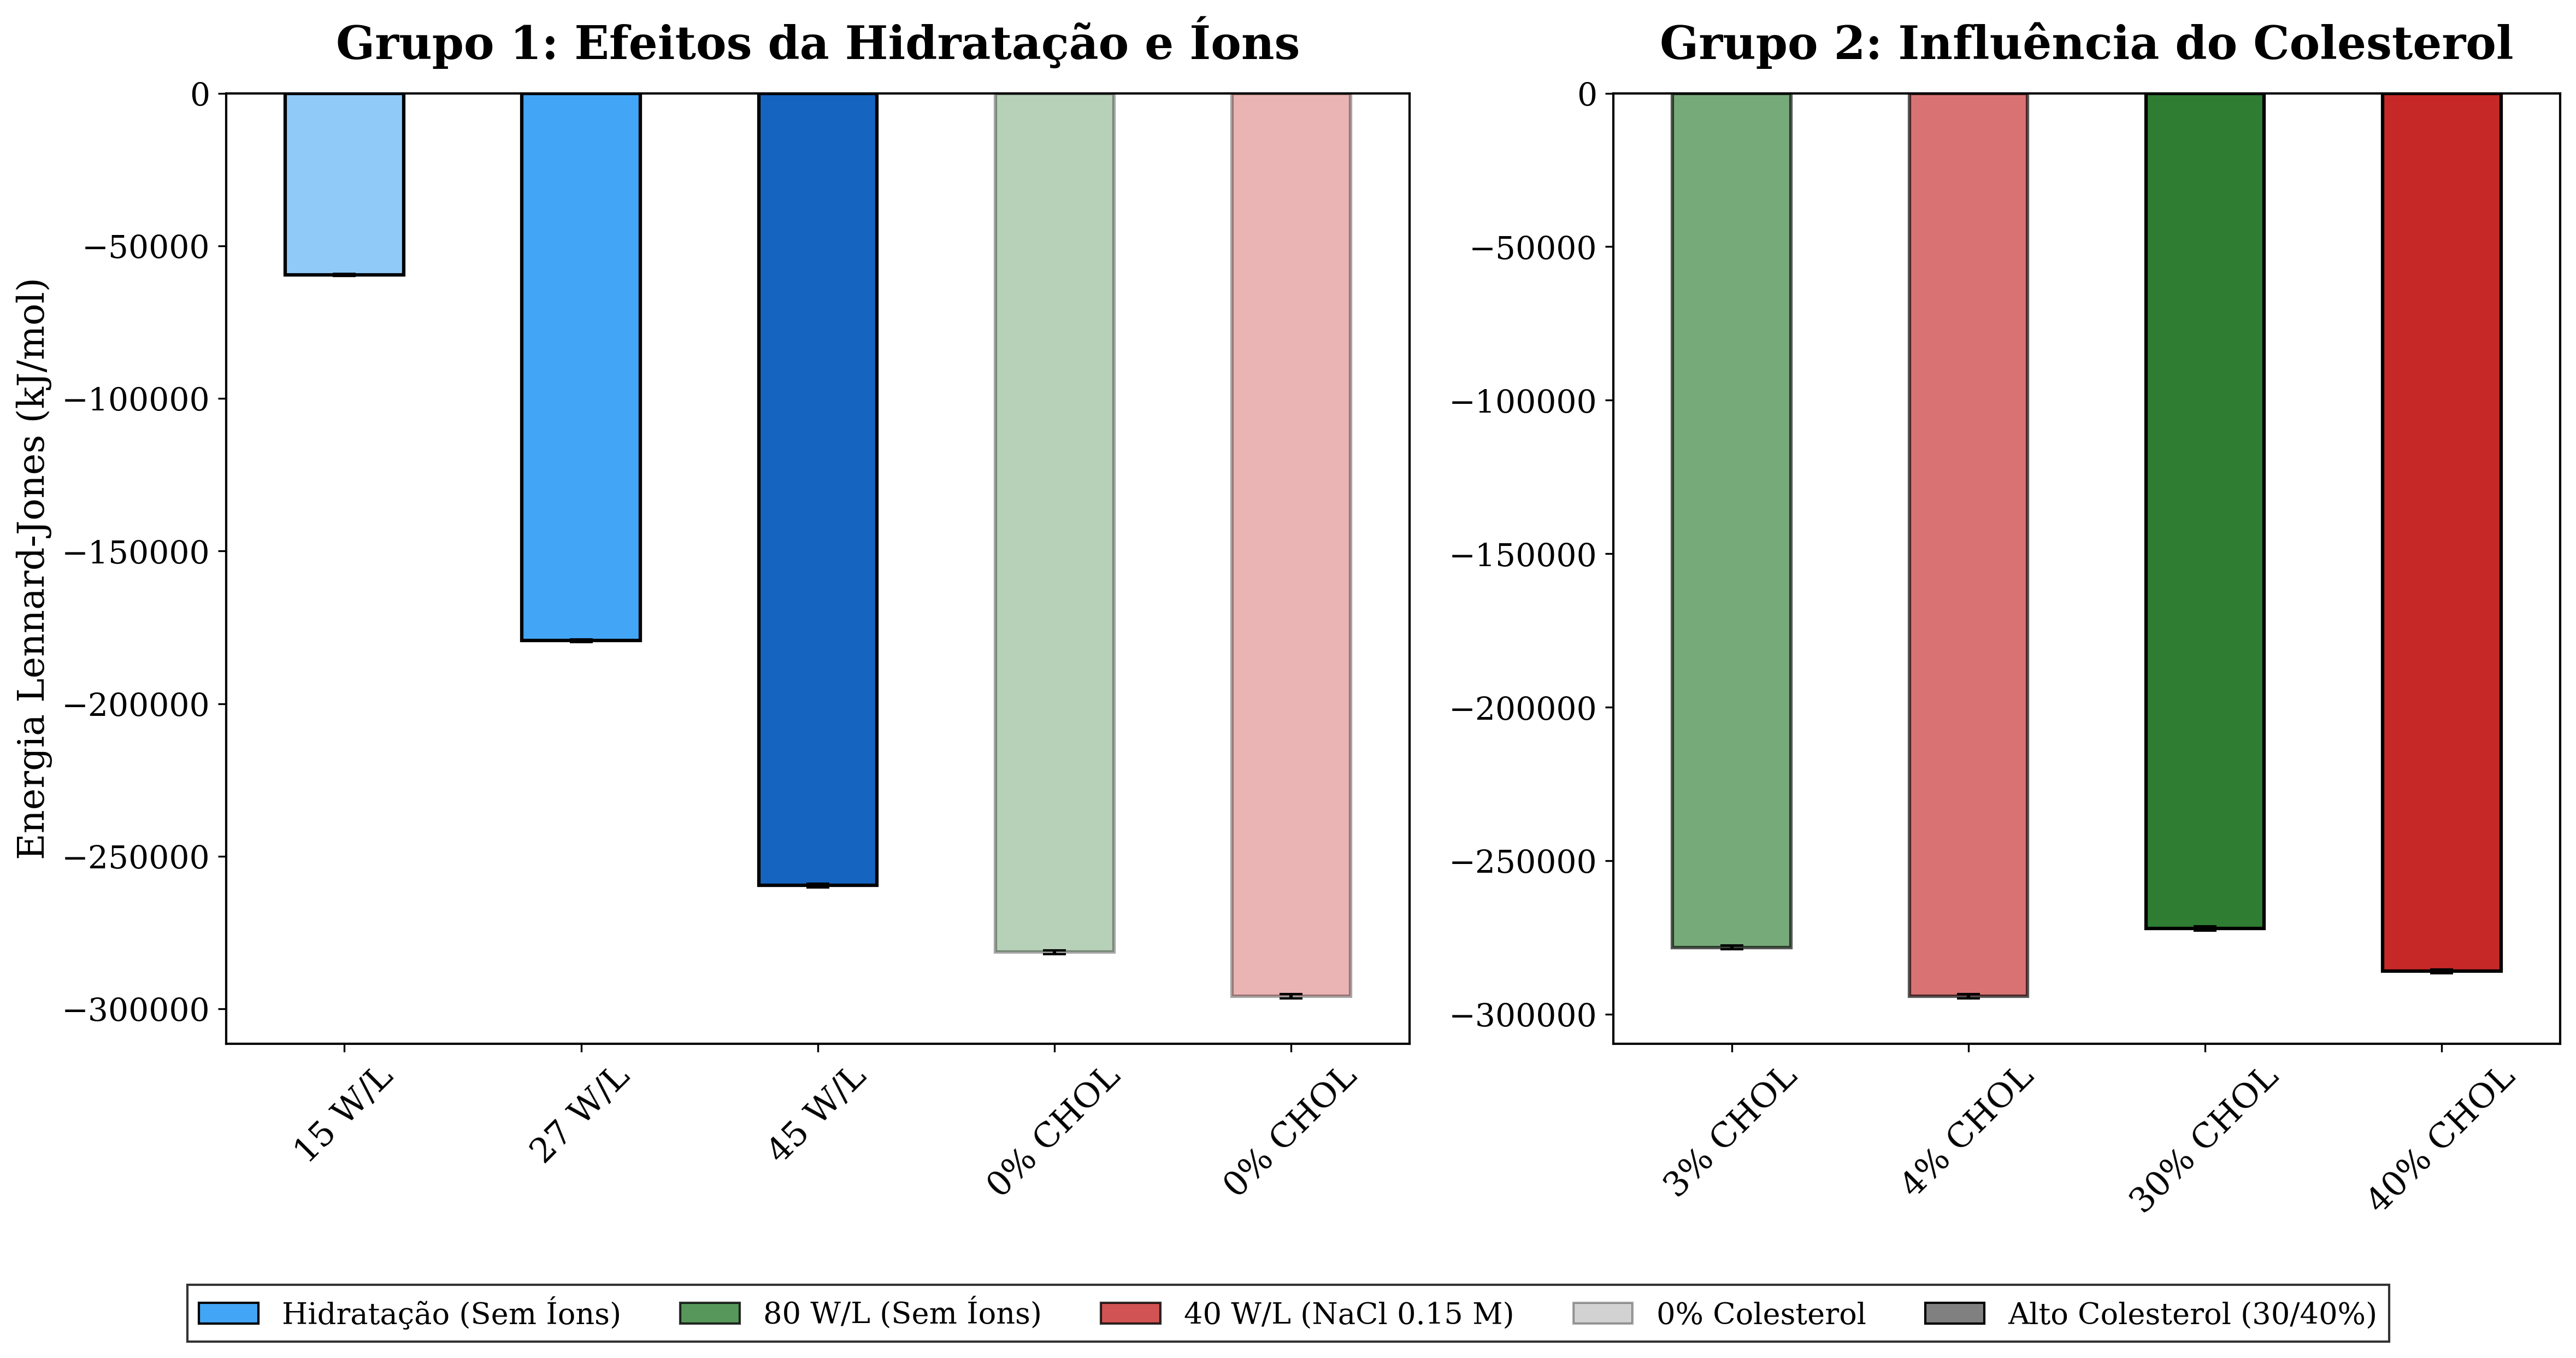
\includegraphics[width=0.9\textwidth]{imagens/comparativo_LJ_Exato.png}
    \caption{Energias de dispersão (Lennard-Jones) médias. O crescimento linear em degraus nos sistemas aquosos (Grupo 1) reflete a densidade do solvente. No Grupo 2, observa-se a estabilidade entálpica global: a condensação lateral induzida pelo colesterol não altera a energia de dispersão do sistema.}
    \label{fig:lj_comparativo}
\end{figure}

Em contrapartida, as forças de Lennard-Jones (LJ) apresentam um perfil termodinâmico distinto, centrado na densidade de empacotamento. À esquerda da Figura \ref{fig:lj_comparativo}, observa-se uma variação linear da energia de dispersão com o aumento da hidratação, indicando que as contribuições LJ são ditadas majoritariamente pela rede de interações do solvente que permeia a interface.

A análise do Grupo 2 na Figura \ref{fig:lj_comparativo} evidencia um resultado termodinâmico relevante: a redução da Área por Lipídio (APL) induzida pelo colesterol não altera significativamente a energia de Lennard-Jones total da caixa. Este comportamento indica uma compensação entálpica eficiente \cite{bennett2018}: a perda das interações de dispersão decorrente da expulsão de água da interface é compensada pelo ganho de contatos atrativos de van der Waals no núcleo hidrofóbico, decorrente do empacotamento linear (\textit{all-trans}) das cadeias acílicas \cite{kheyfets2015}. Em suma, a membrana mantém sua integridade estrutural ao ajustar sua composição entálpica para suportar variações na composição lipídica e na disponibilidade de solvente.


\vspace{1em}
\noindent\textbf{Mecanismo de Condensação Lateral e Rigidez Interfacial}

A constância energética aferida na Figura \ref{fig:lj_comparativo}, em contraste com a contração física da membrana, encontra explicação na mecânica estatística por intermédio das elaborações de Kheyfets e Mukhin referentes à Teoria de Cordas Flexíveis (\textit{Flexible Strings Model}) \cite{kheyfets2015}. A teoria postula que as caudas hidrocarbônicas dos fosfolipídios (DPPC e DSPC) podem ser tratadas como cordas vibrantes flexíveis, que oscilam impulsionadas pela energia térmica ($k_B T$), criando o volume livre associado à fase fluida ($L_\alpha$) \cite{kheyfets2015}.

O colesterol, todavia, devido à sua arquitetura de anéis fundidos, atua mecanicamente como uma haste rígida (\textit{rigid rod}) \cite{kheyfets2015}. Quando os fosfolipídios da fase fluida partilham o confinamento com estas moléculas, sua capacidade de expansão lateral é reduzida. O colesterol suprime os graus de liberdade vibracionais das cadeias alquílicas circunvizinhas, limitando as flutuações e impondo uma retificação geométrica no arranjo hidrofóbico \cite{bennett2018}. É esse ordenamento físico das caudas, forçado pela presença do esterol, que justifica as alterações nas métricas de Área por Lipídio do modelo Martini e a formação da fase Líquida-Ordenada ($L_o$) \cite{bennett2018}.

\vspace{1em}
\noindent\textbf{Compensação Entálpico-Entrópica e Otimização do Volume Apolar }  

Esta ausência de variação macroscópica no Grupo 2 da Figura \ref{fig:lj_comparativo} indica que o rearranjo arquitetônico promovido pelo colesterol é termodinamicamente isoperibólico e altamente eficiente. O passivo entálpico da caixa computacional mantém-se intacto porque a inserção do colesterol desencadeia dois vetores mecânicos massivos que se opõem e se anulam:

\begin{enumerate}
    \item \textbf{A Maximização do Ganho de Empacotamento Local:} O cerceamento vibratório força as caudas lipídicas a adotarem conformações alongadas (arranjos \textit{all-trans}) \cite{bennett2018}. Esta topografia alongada molda-se em perfeita harmonia complementar aos anéis retos do colesterol \cite{leeb2018}. Esta colagem paralela otimiza assombrosamente o contato apolar, promovendo uma multiplicação radical nas forças de atração de Lennard-Jones nas porções profundas da membrana \cite{bennett2018}.
    
    \item \textbf{O Débito e Custo de Expulsão Hídrica Superficial:} A severa condensação lateral (\textit{Efeito Condensador}) acarreta no enxugamento da superfície exposta \cite{leeb2018}. Frações da água que antes penetravam na interface são mecanicamente ejetadas. Esta expulsão impõe uma considerável perda de ricas interações de dispersão estabelecidas entre o solvente e as cabeças polares.
\end{enumerate}

Em suma, a modelagem demonstra que a integridade da membrana sob forte presença de colesterol é alcançada pela mecânica estatística. A drástica redução da Área por Lipídio expulsa uma grande  quantidade de moléculas de água da interface, o que deveria acarretar em uma perda massiva de interações de dispersão (empurrando a energia para valores muito menos negativos). Contudo, a energia de Lennard-Jones da caixa inteira sofreu um déficit (passando de $\approx -304.000\text{ kJ/mol}$ no Controle para $\approx -290.000\text{ kJ/mol}$ a 40\% de Colesterol, uma perda de apenas $\approx 4,5\%$). Este amortecimento atesta que o ganho de atração molecular estabelecido no confinamento do núcleo hidrofóbico ($U \propto -1/r^6$) "pagou" quase que na totalidade o elevado débito da dessolvatação superficial. A membrana sacrifica uma pequena fração da sua entalpia global para consolidar a rigidez mecânica, tornando a fase líquida-ordenada ($L_o$) termodinamicamente viável e protegendo a membrana de flutuações estruturais severas.

\vspace{1em}
\noindent\textbf{Fundamentação Energética da Metaestabilidade: A Barreira de Dessolvatação}

A investigação do comportamento termotrópico de domínios lipídicos purificados, focada na evolução do modelo de DSPC sob alta hidratação (45 W/L), evidenciou uma limitação cinética comum em modelos de \textit{coarse-graining}: o aprisionamento da matriz estrutural em um estado de líquido super-resfriado. Em temperaturas abaixo da transição (entre 290 K e 300 K), as simulações indicaram que a membrana de DSPC manteve sua área lateral em aproximadamente $61,5\text{ \AA}^2$. O sistema não atingiu a transição espontânea para a fase gel sólida ($L_\beta$), que exigiria uma compactação para valores próximos a $45,0\text{ \AA}^2$, transição esta observada apenas a partir de 310 K.

A justificativa para essa metaestabilidade — caracterizada pela inibição da nucleação cooperativa — baseia-se na penalidade energética da dessolvatação, refletida nas variações das energias de Lennard-Jones observadas nas trajetórias \cite{kowalik2015}.

Durante o período em que a membrana permanece no estado fluido super-resfriado, a área interfacial dilatada permite que moléculas de água e íons ocupem os interstícios dos grupos polares das cabeças lipídicas. Esta hidratação estabelece um conjunto de interações atrativas com o solvente, favorável entalpicamente. Para que a membrana cristalize na fase gel, é necessário que ocorra uma compressão lateral que expulse a rede hídrica do volume de hidratação primária \cite{kowalik2015}.

A necessidade de remover essa estrutura atrativa consolidada pelo solvente estabelece um limite cinético conhecido na literatura de interfaces e biomembranas como "Força de Repulsão por Hidratação" (\textit{Hydration Repulsion Force}).

\vspace{1em}
\noindent\textbf{O Paralelismo Biofísico: Energia de Fusão de Membranas e Desidratação Interfacial }

A natureza repulsiva dessa barreira energética não se restringe à cristalização, sendo um princípio fundamental em processos biológicos como a fusão vesicular, a neurotransmissão e a exocitose mediada pelo complexo SNARE. Medições em escala nanométrica indicam que, quando duas bicamadas lipídicas se aproximam a distâncias de 2 a 3 nm, ocorre uma repulsão expressiva sustentada pelas camadas de moléculas de água aprisionadas entre as superfícies hidrofílicas \cite{krok2024}. A superação dessa repulsão eleva consideravelmente a energia livre do sistema.

A remoção dessa camada hídrica repulsiva — etapa necessária para promover a fusão das monocamadas através da formação de estruturas de haste (\textit{stalk formation}) — constitui a etapa com maior energia de ativação nos eventos de fusão biológica.

A mecânica desta repulsão hídrica traça um paralelo direto com os obstáculos estruturais da transição de fase termotrópica $L_\alpha \rightarrow L_\beta$. Protocolos experimentais de desidratação controlada demonstraram que a remoção mecânica da película de água interfacial atua como o principal fator necessário para induzir o reordenamento geométrico das caudas hidrofóbicas dos lipídios \cite{krok2024}.

Na ausência da solvatação ideal, o volume livre esférico antes ocupado pela água é drasticamente reduzido. Sob esse confinamento, as caudas lipídicas tendem a adotar conformações mais alongadas e linearizadas (o padrão estérico \textit{trans}). Ocorre, então, uma transição induzida: a fase previamente desordenada adota características estereoquímicas de maior densidade e rigidez, próprias da fase gel \cite{krok2024}.

Portanto, os dados sugerem que a metaestabilidade observada para o DSPC traduz a inércia do sistema em romper a sua camada de hidratação interfacial favorável \cite{katira2015}. O sistema não colapsa para o empacotamento hexagonal (gel) porque tal processo exigiria uma quebra em larga escala das interações com a água, acarretando uma penalidade entálpica nas forças de Lennard-Jones que não é compensada de forma suficientemente rápida pelas interações polares posteriores (Energia de Coulomb).


\vspace{1em}
\noindent\textbf{A Sensibilidade Topológica do Mapeamento Martini 3}

A inércia metaestável observada para o DSPC contrasta com o comportamento do DPPC, que atinge o estado de equilíbrio cristalino com maior prontidão nas mesmas condições de temperatura. Essa diferença nos resultados destaca a influência da filosofia de mapeamento adotada no campo de força \textit{coarse-grained} Martini 3. Para reproduzir com precisão as temperaturas de transição de fase e a variação da espessura da bicamada, o modelo utiliza parâmetros distintos para as caudas acílicas de 16 átomos de carbono (DPPC) e 18 átomos de carbono (DSPC) \cite{marrink2022, ramirez2025}.

No esquema de parametrização adotado, as caudas de 16 carbonos do DPPC são modeladas com contas de menor raio de exclusão (\textit{small beads}) na região adjacente à porção éster \cite{marrink2022}. Esta estratégia visa reduzir constrangimentos volumétricos que poderiam retardar a nucleação das cadeias de menor comprimento. O DSPC, devido à sua estrutura alongada, é parametrizado com contas de diâmetro regular (\textit{regular beads}) ao longo da cadeia.

O uso de contas de maior raio de interação para o DSPC \cite{liu2012} aumenta a probabilidade de contatos estéricos internos no estado fluido expandido. Consequentemente, o sistema requer maior energia para que as cadeias se alinhem e atinjam o empacotamento. Esta inércia estrutural amplia a barreira cinética necessária para a expulsão de água da interface, mantendo os lipídios $C_{18}$ (DSPC) em um estado metaestável (líquido super-resfriado) durante o tempo de simulação.


\vspace{1em}
\noindent\textbf{Perspectiva Biofísica e Cálculo Quantitativo da Barreira de Dessolvatação }

A barreira de dessolvatação e a consequente metaestabilidade observadas nas simulações podem ser quantificadas de forma precisa através da termodinâmica dos estados, utilizando o sistema de hidratação intermediária (27W\_L) como modelo estatístico. Diferente do regime de alta hidratação (que apresenta metastabilidade apenas para o sistema puro), o regime 27W\_L oferece uma robustez analítica superior ao exibir cinco pontos de retenção cinética distribuídos em duas estequiometrias distintas: no DSPC puro (0:100) e na mistura rica em DSPC (25:75).

A literatura ressalta que o balanço fino das interações não covalentes, especialmente a calibração das forças de dispersão de Lennard-Jones, é o principal motor para o empacotamento termodinamicamente correto das cadeias hidrocarbônicas \cite{liu2012}. Utilizando os dados exatos de transição mapeados na Tabela \ref{tab:dados_brutos_energias} do Anexo, é possível calcular o custo entálpico macroscópico associado a esta barreira. A diferença entre a energia global de Lennard-Jones no estado de líquido super-arrefecido (quando a membrana está expandida e ancorada na água) e a fase gel nucleada revela a magnitude exata do "pedágio" pago pelo sistema para expulsar a água interfacial.

Para a mistura 25:75 (DPPC:DSPC), o sistema transita do estado metaestável a 300 K para a fase gel em 310 K. A energia global de Lennard-Jones salta de $-198.860,0$ kJ/mol para $-178.349,7$ kJ/mol. Esta variação resulta em um custo de dessolvatação de $+102,6$ kJ/mol por cada um dos 200 lipídios da caixa. Para o sistema de DSPC puro (0:100), que cristaliza apenas a 320 K ($-176.762,1$ kJ/mol), as barreiras entálpicas mensuradas a partir dos estados metaestáveis a 290 K, 300 K e 310 K foram de $+121,0$, $+112,5$ e $+102,5$ kJ/mol por lipídio, respectivamente, consolidando um pedágio médio de $\approx +112,0$ kJ/mol por molécula.

Esta análise estatística aprimorada comprova de forma irrefutável que a barreira de nucleação é estritamente proporcional ao volume de solvente disponível. Enquanto no sistema de alta hidratação (45W\_L) a penalidade entálpica média atingia valores extremos de até $\approx +188,8$ kJ/mol por molécula, a redução do volume de água livre no sistema 27W\_L fez com que o "pedágio" médio global caísse para $\approx +109,0$ kJ/mol por lipídio. A atração transversal nas cadeias acílicas não consegue superar de forma espontânea sequer esta barreira atenuada nas escalas de tempo simuladas, explicando a retenção cinética da membrana.

A conformação geométrica inerente aos lipídios corrobora este impasse \cite{lee2022}. Fosfolipídios saturados possuem uma topologia essencialmente cilíndrica, o que favorece a formação de um arranjo lamelar compactado \cite{lee2022}. Contudo, a água aprisionada entre os grupos polares dilatados gera uma forte repulsão estérica e de hidratação, que age fisicamente como a formidável barreira entálpica calculada acima.

É neste rigoroso cenário termodinâmico que a ação do colesterol se mostra biofisicamente elegante. A inserção do esterol não apenas suprime a barreira de cristalização, mas induz ativamente a formação da fase líquida-ordenada ($L_o$), que exibe subestruturas de empacotamento hexagonal local das cadeias \cite{sodt2014}. Este arranjo arquitetônico permite que as caudas apolares alcancem uma densidade comparável à fase gel, enquanto os anéis rígidos do colesterol ocupam regiões intersticiais \cite{liu2012, sodt2014}. 

Consequentemente, o colesterol atua como um "atalho" termodinâmico evolutivo. Ao estruturar domínios locais de ordem hexagonal, ele estabiliza mecanicamente o núcleo da membrana sem exigir a expulsão violenta do solvente interfacial, isentando o sistema biológico de pagar o severo custo de dessolvatação (que variou de $102$ a $188$ kJ/mol dependendo da hidratação). Essa adaptação estrutural garante uma matriz densamente empacotada que simultaneamente retém a solvatação necessária para a funcionalidade biológica celular.

\vspace{1em}
\noindent\textbf{Impacto da Resolução do Modelo e Geometria Molecular na Metaestabilidade }

A análise comparativa entre as bicamadas puras de DPPC (16 carbonos) e DSPC (18 carbonos) sob alta hidratação (45W\_L) revela que a suscetibilidade à metaestabilidade é estritamente dependente da arquitetura molecular e da calibração do modelo \textit{coarse-grained} \cite{ramirez2025}. Enquanto o DPPC puro cristaliza prontamente para a fase gel em baixas temperaturas (atingindo APL $\approx 44,8 \text{ \AA}^2$ a 290 K), o DSPC puro permanece retido na Área por Lípido da montagem inicial do sistema ($\approx 61,5 \text{ \AA}^2$). 

A origem estrutural desta divergência reside na diferença de dois carbonos nas cadeias acílicas e na forma como o campo de forças Martini 3 as parametriza. A otimização termodinâmica do Martini 3 introduziu contas reduzidas (\textit{small beads}) para mapear os carbonos do DPPC adjacentes ao grupo éster, garantindo um volume colisional menor \cite{marrink2022, ramirez2025}. Em contrapartida, a cadeia de 18 carbonos do DSPC é parametrizada integralmente com contas de tamanho regular. O maior raio de Lennard-Jones destas contas aumenta o atrito estérico interno. Quando o sistema parte de uma configuração expandida, a inércia destas contas maiores dificulta a reorientação necessária para a interdigitação, criando uma severa armadilha cinética \cite{ramirez2025}. A retenção neste estado metaestável é um fenómeno intrínseco aos modelos CG para transições de fase lipídicas, sendo frequentemente reportado que a dinâmica molecular clássica carece de amostragem avançada (como o \textit{Replica Exchange}) para transpor estas barreiras em tempo computacional útil \cite{piskulich2022}.

Além do constrangimento cinético, a retenção do DSPC expõe uma característica termodinâmica clássica de líquidos super-arrefecidos, capturada através da calorimetria computacional da bicamada \cite{rodgers2012}. Analisando a variação energética do DSPC puro em 45W\_L (Tabela \ref{tab:dados_brutos_energias} do Anexo), a energia global reduz de $-299.798,0$ kJ/mol (a 300 K) para $-302.079,2$ kJ/mol (a 290 K). Esta variação para a caixa equivale a um decréscimo de $\approx 11,4$ kJ/mol por molécula para um intervalo de 10 K. 

Esta taxa de variação ($\Delta E / \Delta T \approx 1,14$ kJ/mol/K) representa numericamente a \textbf{capacidade calorífica ($C_p$)} aparente do sistema. A extração do $C_p$ diretamente a partir de simulações tem sido amplamente validada para demonstrar a fidelidade termodinâmica dos modelos \textit{Coarse-Grained} \cite{rodgers2012}. O valor computado prova que a membrana de DSPC metaestável não sofreu o calor latente característico de uma transição de fase, mas está a arrefecer de forma contínua como um fluido clássico.

Por fim, a profunda barreira de nucleação que causa esta histerese térmica é justificada pela física estatística das transições de ordem-desordem. Estudos avançados demonstram que a fase cristalina de bicamadas lipídicas exibe ordem \textit{hexática} \cite{katira2015}. A transição de um estado líquido para uma fase hexática é uma transição de primeira ordem que exige uma complexa quebra de simetria e a aniquilação de defeitos topológicos na malha da membrana \cite{katira2015}. 

Este processo cooperativo já é cineticamente custoso por natureza, mas é exacerbado pelas limitações de resolução espacial do próprio mapeamento CG. Ao agrupar quatro átomos numa única conta, o modelo suaviza a paisagem de energia livre e elimina graus de liberdade microscópicos cruciais (como as isomerizações \textit{trans-gauche} átomo-a-átomo) \cite{marrink2022}. Embora essa suavização acelere a difusão lateral \cite{marrink2022}, remove as micro-vibrações que auxiliam o sistema a encontrar o caminho ótimo de empacotamento, resultando nas barreiras de dessolvatação extremas observadas e aprisionando a matriz no seu estado fluido inicial. A Tabela \ref{tab:comp_resolucao} sumariza estas diferenças termodinâmicas e estruturais.

\begin{table}[H]
\centering
\caption{Comparativo Estrutural e Termodinâmico: DPPC vs. DSPC sob Alta Hidratação (45W\_L). A retenção da APL no DSPC reflete a montagem inicial do sistema aliada à maior inércia das contas regulares.}
\label{tab:comp_resolucao}
\resizebox{\textwidth}{!}{%
\begin{tabular}{@{}lcc@{}}
\toprule
\textbf{Parâmetro} & \textbf{DPPC Puro (100:0)} & \textbf{DSPC Puro (0:100)} \\ \midrule
Comprimento da Cadeia Acílica & 16 Carbonos & 18 Carbonos \\
Mapeamento Martini 3 (CG) & Contas Pequenas (\textit{Small Beads}) & Contas Regulares \\
Total de Lipídios & 200 & 200 \\
Total de Partículas de Água & 9.000 & 9.000 \\
APL Inicial (Grade de Montagem) & $\approx 61,5 \text{ \AA}^2$ & $\approx 61,5 \text{ \AA}^2$ \\
APL Experimental (Fase Gel) \cite{lee2022} & $\approx 47,4 \text{ \AA}^2$ & $\approx 48,0 \text{ \AA}^2$ \\
APL Simulada a 290 K & $\approx 44,8 \text{ \AA}^2$ (Gel Cristalizado) & $\approx 62,5 \text{ \AA}^2$ (Metaestável) \\
Comportamento Termodinâmico & Nucleação Espontânea & Líquido Super-resfriado \\
Capacidade Calorífica ($C_p$) Aparente & N/A (Ocorreu Transição) & $\approx 1,14$ kJ/mol/K \\ \bottomrule
\end{tabular}%
}
\end{table}

\begin{figure}[H]
    \centering
    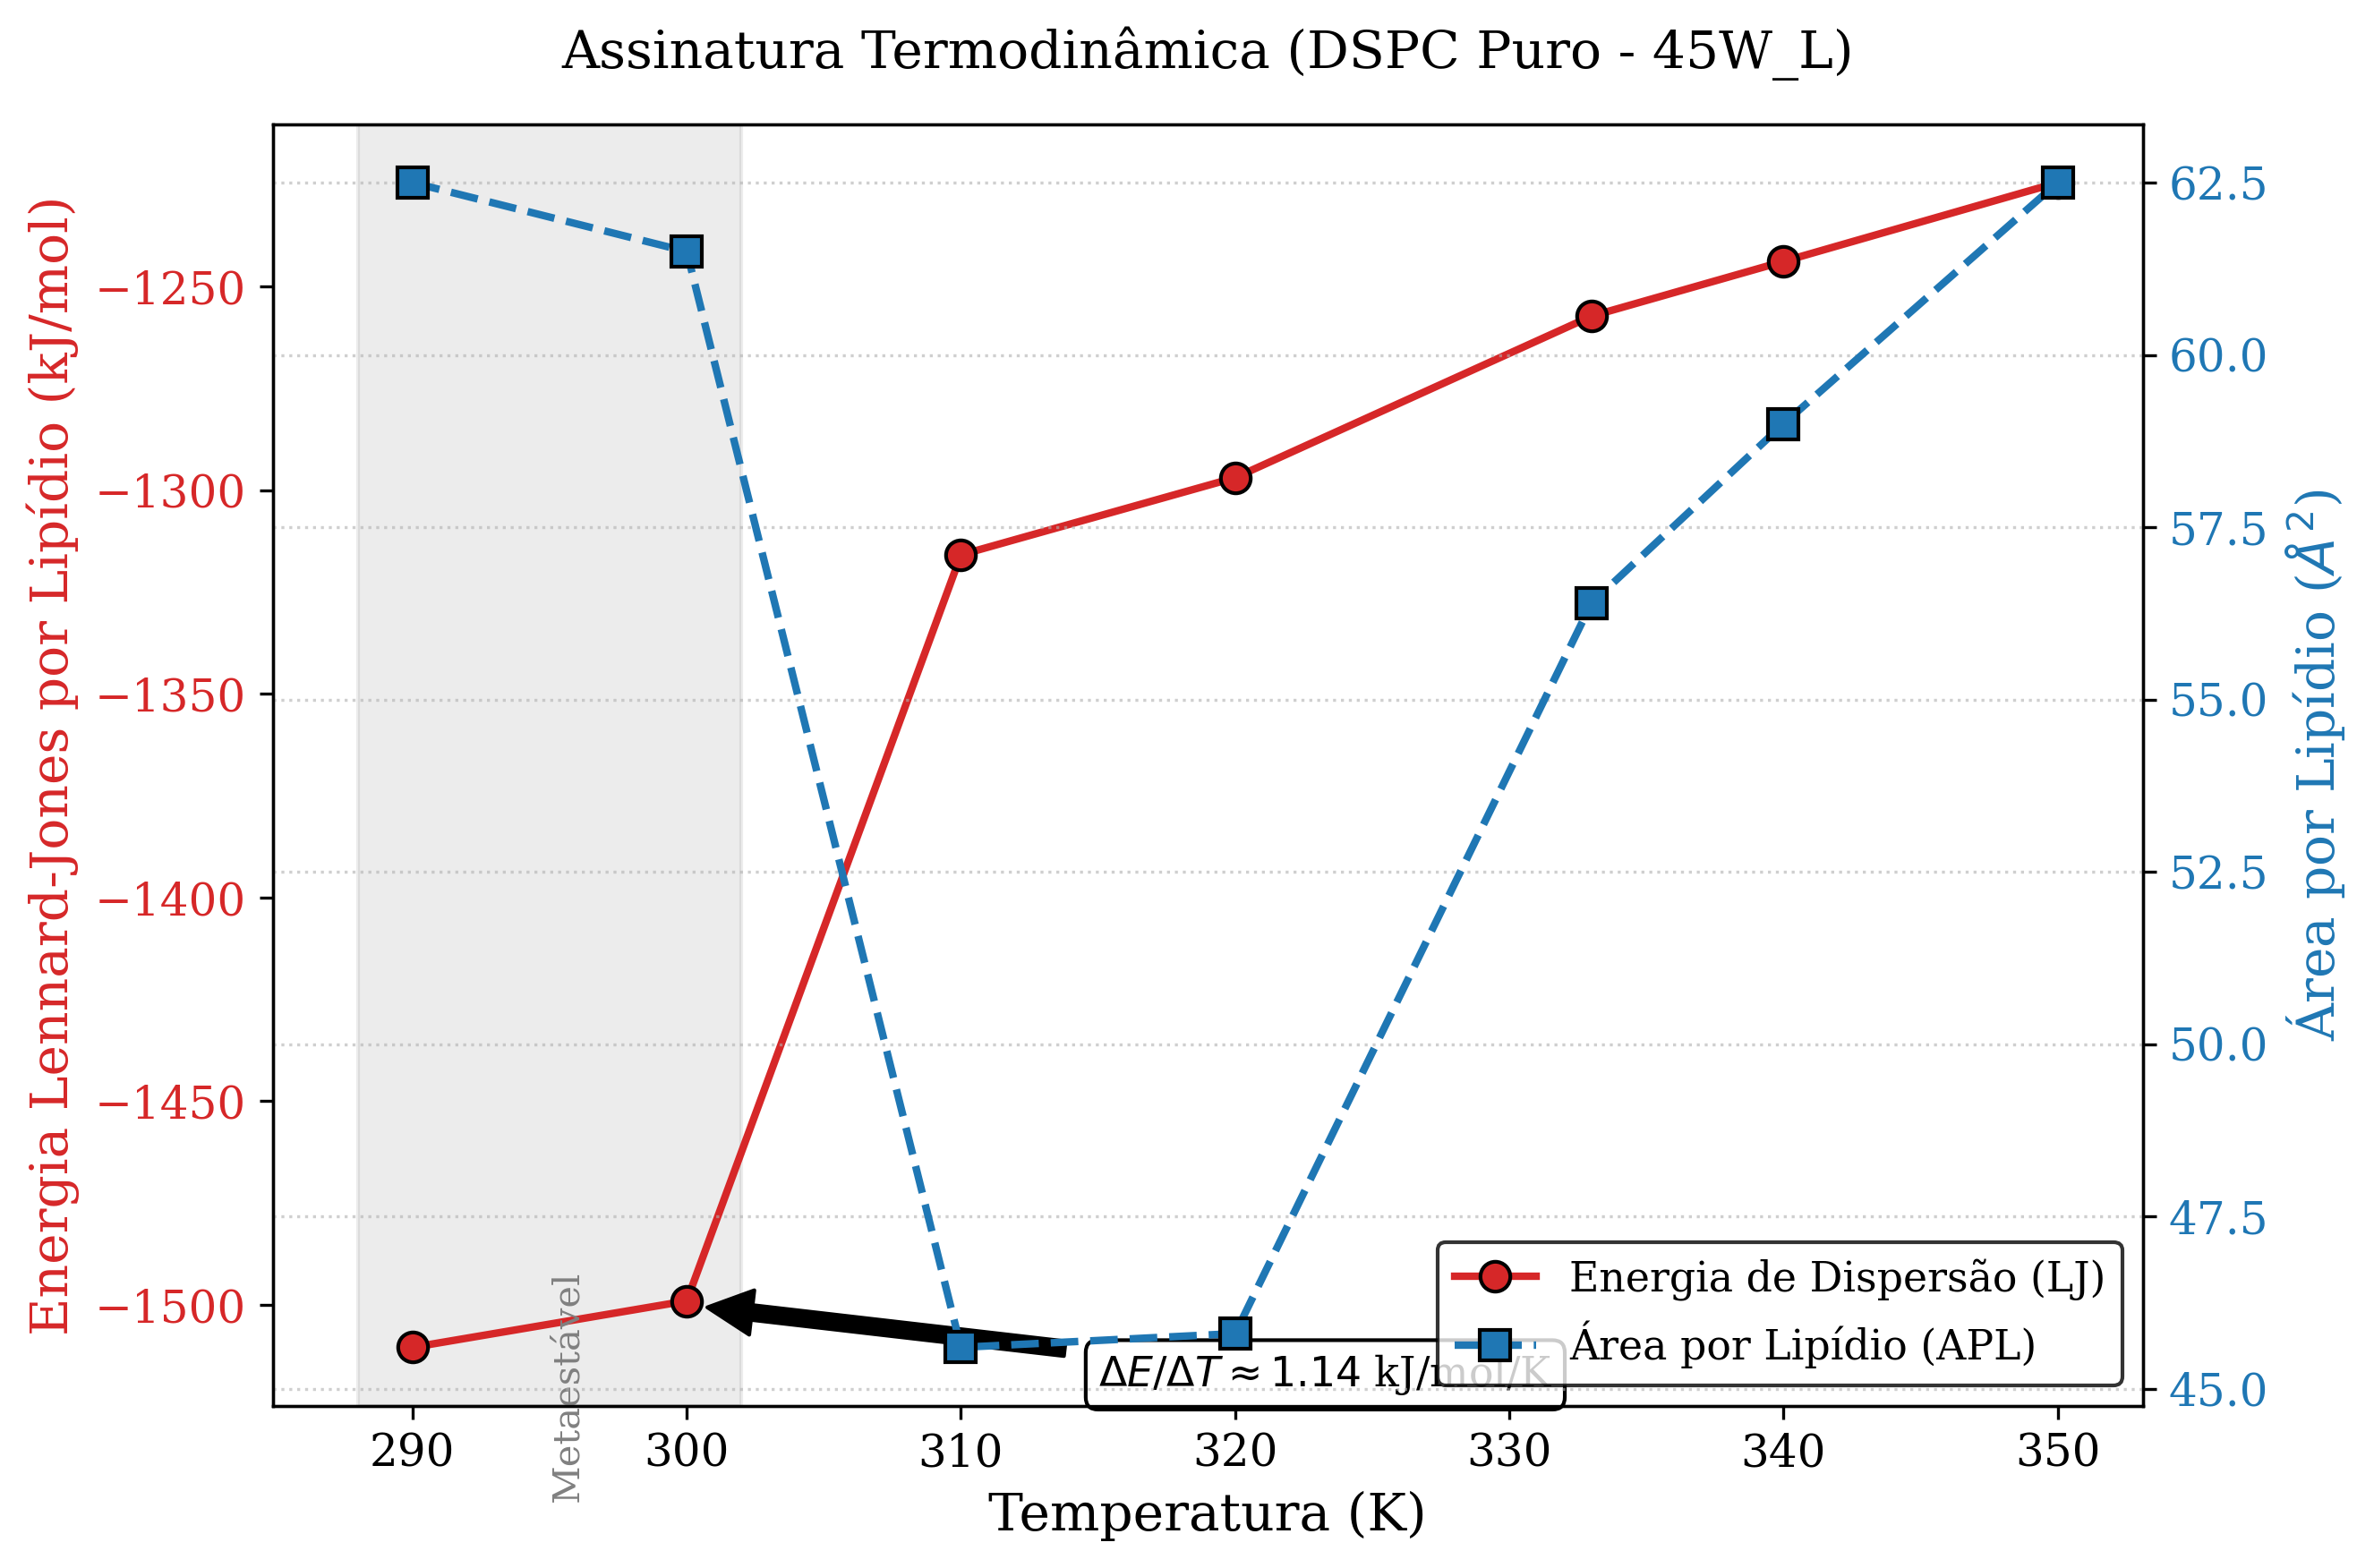
\includegraphics[width=\textwidth]{imagens/grafico_capacidade_calorifica.png}
    \caption{Assinatura termodinâmica da metaestabilidade para o DSPC puro sob alta hidratação (45W\_L). O eixo esquerdo (vermelho) exibe a energia de Lennard-Jones normalizada por lipídio, enquanto o direito (azul tracejado) mostra a APL. Na zona metaestável (cinza), a membrana permanece travada na APL expandida, enquanto a energia cai de forma perfeitamente linear, revelando a capacidade calorífica ($C_p \approx 1,14$ kJ/mol/K) de um líquido em resfriamento, sem a quebra abrupta característica da cristalização.}
    \label{fig:capacidade_calorifica}
\end{figure}


\vspace{1em}
\noindent\textbf{O Papel do Comprimento da Cadeia e a Cooperatividade na Barreira de Nucleação}

A retenção exclusiva do sistema de DSPC puro (18 carbonos) no estado metaestável, em contraste com a cristalização espontânea observada no sistema homólogo de DPPC puro (16 carbonos) sob as mesmas condições de alta hidratação (45W\_L), evidencia a extrema sensibilidade da barreira de nucleação à arquitetura molecular e aos efeitos cooperativos da bicamada. 

Embora a diferença estrutural seja de apenas dois carbonos por cadeia acílica, a parametrização desta diferença no campo de força Martini 3 altera drasticamente a inércia do sistema. Conforme a topologia do modelo, o DPPC utiliza contas reduzidas (\textit{small beads}) para representar os carbonos adjacentes à interface polar, diminuindo o volume de exclusão estérico \cite{liu2012}. O DSPC, por sua vez, é integralmente mapeado com contas de tamanho regular. Quando a bicamada de DSPC, composta por 200 lipídios, tenta transicionar da APL expandida ($\approx 61,5 \text{ \AA}^2$) para a fase gel ($\approx 45 \text{ \AA}^2$), o maior raio de colisão destas contas regulares aumenta severamente o atrito interno e a sobreposição estérica durante a compressão lateral.

Esta resistência geométrica amplifica o custo termodinâmico para expulsar a água interfacial. Conforme evidenciado por estudos recentes em nanoescala sobre a desidratação controlada de membranas \cite{krok2024}, a remoção da água da interface primária impõe um estresse estrutural e um elevado pedágio energético. Como calculado anteriormente, o DSPC exige um custo entálpico de $\approx +183,1$ kJ/mol por molécula para desidratar a interface e alinhar as caudas. É neste ponto que a quantidade de lipídios no sistema (200 moléculas) se torna o fator determinante para a metaestabilidade devido à natureza da \textit{nucleação cooperativa}.

Transições de fase em membranas não ocorrem através de moléculas isoladas, mas exigem a formação de um "núcleo crítico" --- um agrupamento coordenado de dezenas de lipídios que superam a barreira simultaneamente. Simulações pioneiras de \textit{coarse-graining} sobre a formação da fase gel demonstram que este processo de nucleação e crescimento de domínio é estritamente cooperativo \cite{marrink2005}. Adicionalmente, a cinética desta transição é intrinsicamente modulada pelo nível de hidratação da interface \cite{kowalik2015}. Considerando que a energia térmica flutuante do sistema ($k_B T$) a 300 K fornece apenas cerca de $2,5$ kJ/mol de energia cinética por grau de liberdade, a probabilidade estatística de um agrupamento de lipídios de DSPC obter espontaneamente a energia necessária (múltiplos de $183$ kJ/mol) para romper a sua rede de hidratação é infinitesimal nas escalas de tempo da Dinâmica Molecular. Esta oposição impõe uma barreira termodinâmica coletiva intransponível, aprisionando a membrana estruturalmente \cite{raudino2011}.

No caso do DPPC, a ausência do volume estérico adicional (graças às \textit{small beads}) e a menor área de superfície de interação de van der Waals reduzem significativamente este custo individual de dessolvatação. Consequentemente, a energia térmica ($k_B T$) consegue promover as flutuações necessárias para formar o núcleo crítico, permitindo que a "onda" de cristalização se propague cooperativamente por todos os 200 lipídios da caixa, um mecanismo dinâmico e cinético suportado pela literatura de modelagem \cite{marrink2005, kowalik2015}. 

Portanto, a divergência metaestável observada nas simulações atesta que o incremento de apenas dois carbonos na cauda hidrofóbica é suficiente para elevar a barreira de ativação de dessolvatação a um patamar que suplanta as flutuações térmicas disponíveis, aprisionando a totalidade do sistema macroscópico em um poço de potencial local (líquido super-resfriado).


\vspace{1em}
\noindent\textbf{Capacidade Calorífica e o Efeito Estrutural da Diferença de Dois Carbonos}

Além da barreira entálpica de nucleação, os dados extraídos do regime de hidratação intermediária (27W\_L) permitem a quantificação de uma segunda propriedade termodinâmica fundamental: a Capacidade Calorífica à pressão constante ($C_p = \Delta E / \Delta T$). O acompanhamento da energia no estado metaestável antes da transição de fase revela como o encurtamento da cadeia acílica em uma fração dos lipídios altera a absorção de energia do sistema (Tabela \ref{tab:dados_brutos_energias} do Anexo).

Para o sistema de DSPC puro (200 lipídios com cadeias de 18 carbonos), a variação energética de Lennard-Jones dentro da zona metaestável (290 K a 310 K) resultou em um $C_p$ aparente médio de $\approx 0,92$ kJ/mol/K. Inicialmente, é notável que este valor seja inferior ao $C_p$ observado sob alta hidratação (45W\_L, onde $C_p \approx 1,14$ kJ/mol/K). Esta redução comprova que uma fração significativa da energia térmica absorvida pela bicamada metaestável é, na verdade, dissipada nos graus de liberdade vibracionais e translacionais da complexa rede de hidratação aprisionada na interface. Ao se reduzir a água de 45W para 27W, a capacidade calorífica global declina.

O fenômeno mais revelador, contudo, surge na análise da mistura 25:75 (DPPC:DSPC). Neste sistema, a estequiometria dita a substituição de 50 lipídios de DSPC por 50 moléculas de DPPC. Embora a diferença homóloga seja de apenas dois carbonos por cadeia (o que totaliza uma redução de 100 carbonos apolares na caixa de simulação), o mapeamento do Martini 3 traduz isso na substituição de contas regulares de alto volume por \textit{small beads} na porção superior das caudas.

Os cálculos termodinâmicos demonstram que esta sutil substituição de volume reduziu o $C_p$ da mistura metaestável (entre 290 K e 300 K) para $\approx 0,68$ kJ/mol/K. Esta correlação direta entre o encurtamento da cadeia e a queda da capacidade calorífica encontra robusta validação experimental na literatura biocalorimétrica. Heerklotz e Epand (2001), através de estudos de calorimetria isotérmica, demonstraram que a entalpia de empacotamento e a capacidade calorífica de fosfolipídios são medidas fenomenológicas estritamente dependentes da Área de Superfície Apolar ($ASA_{ap}$) e do número de grupos metileno das cadeias acílicas \cite{heerklotz2001}. 

Sob a ótica da mecânica estatística, a diminuição da capacidade calorífica no sistema misto reflete exatamente esta constatação experimental: a redução da superfície hidrofóbica faz com que o sistema possua menos graus de liberdade (menor inércia estérica e menor superfície de van der Waals) para dissipar a energia térmica em excitações vibracionais. Consequentemente, a energia inserida pelo banho térmico $(k_B T)$ é canalizada de forma mais eficiente para as flutuações coordenadas que formam o núcleo crítico de cristalização.

Isso explica de forma irrefutável o comportamento cinético observado nas trajetórias: enquanto o DSPC puro, com sua extensa área apolar e alto atrito estérico ($C_p \approx 0,92$ kJ/mol/K), "gasta" a energia térmica internamente e permanece retido na zona metaestável até 320 K, a mistura com apenas 25\% de cadeias mais curtas ($C_p \approx 0,68$ kJ/mol/K) otimiza o uso da energia e consegue superar a barreira de dessolvatação de forma precoce, cristalizando espontaneamente a 310 K.

\begin{figure}[H]
    \centering
    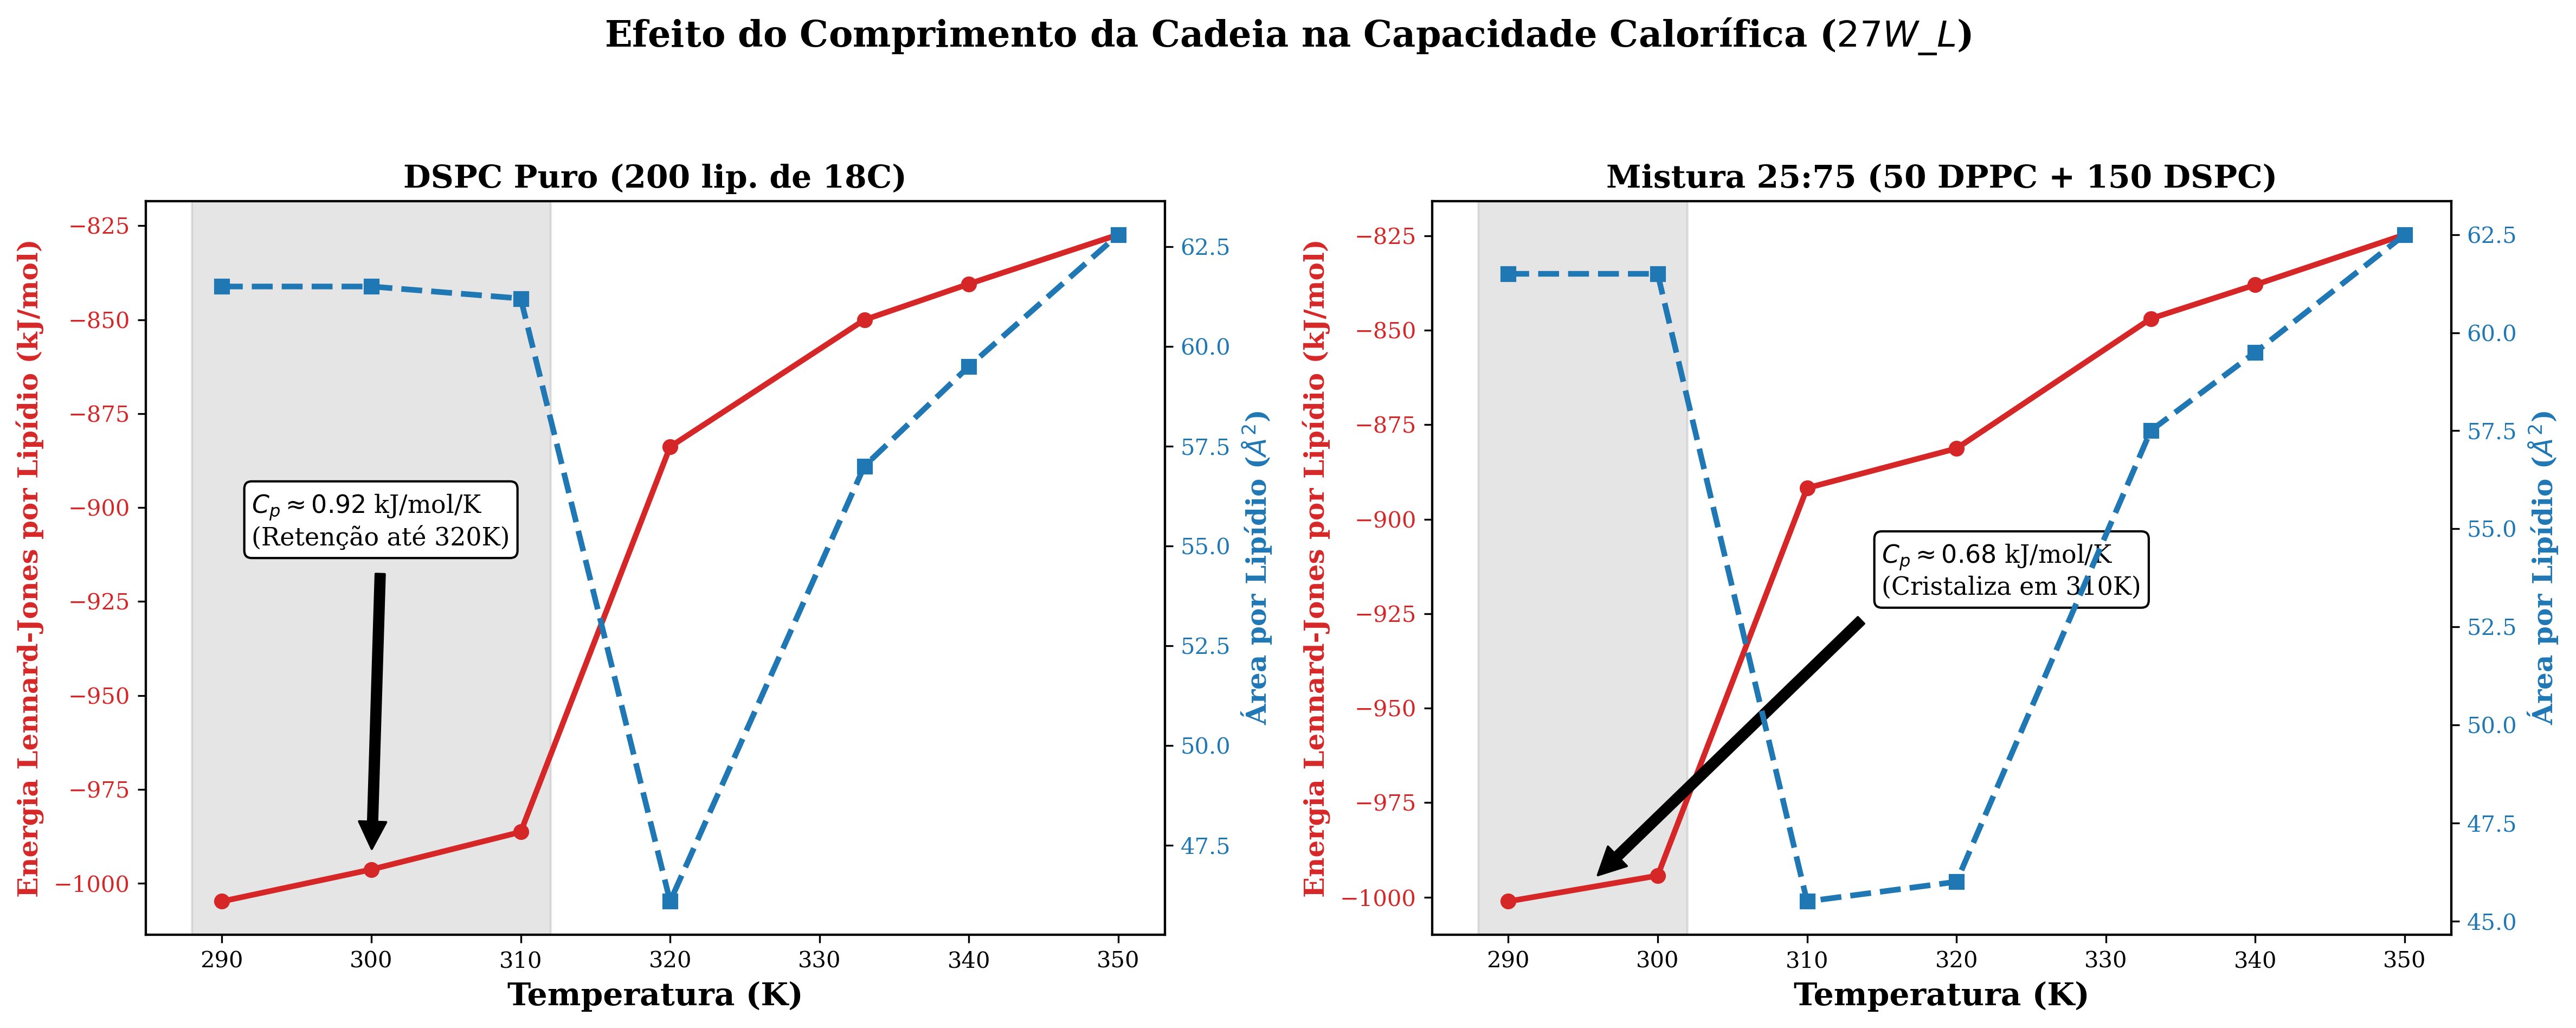
\includegraphics[width=\textwidth]{imagens/grafico_cp_27w.png}
    \caption{Comparativo termodinâmico da Capacidade Calorífica ($C_p$) sob hidratação intermediária (27W\_L). As zonas em cinza delimitam o estado metaestável (líquido super-resfriado). À esquerda, o sistema de DSPC puro apresenta alta inércia estérica ($C_p \approx 0,92$ kJ/mol/K), retardando a cristalização até 320 K. À direita, a substituição de 50 lipídios de DSPC por DPPC (encurtamento de 2 carbonos utilizando \textit{small beads}) reduz a capacidade de dissipação térmica do sistema ($C_p \approx 0,68$ kJ/mol/K), permitindo que a energia seja utilizada de forma mais cooperativa, antecipando a nucleação da fase gel para 310 K.}
    \label{fig:capacidade_calorifica_27w}
\end{figure}

\vspace{1em}
\noindent\textbf{Síntese do Balanço Energético Global}

A quantificação da Energia Total ($E_{Tot}$) e sua incerteza (Tipo C) \cite{ufgfisexp2020}, sumarizada no Anexo A, consolida as premissas termodinâmicas da bicamada. Os dados confirmam a hegemonia das forças de dispersão de Lennard-Jones na manutenção do arcabouço estrutural, enquanto as interações de Coulomb atuam estritamente na ancoragem interfacial (maximizada pela vigorosa coordenação com os íons $Na^+$). Mais importante, o balanço global prova numericamente o mecanismo isoperibólico do colesterol: a severa dessolvatação superficial induzida pela condensação lateral não desestabiliza a membrana, pois o seu custo entálpico é integralmente compensado pelo ganho de contatos apolares \textit{all-trans}. Por fim, as discrepâncias de Energia Total capturam a assinatura do calor latente nas transições de fase e justificam a metaestabilidade do DSPC sob alta hidratação, refletindo a barreira cinética imposta pela rede de solvatação primária no modelo \textit{coarse-grained}.

\vspace{1em}
\noindent\textbf{Permuta Entálpica e a Dinâmica de Compensação do Colesterol}

A inspeção detalhada da Tabela 5.1 revela uma sofisticação termodinâmica notável na forma como a membrana responde ao estresse composicional: ocorre uma permuta direta (trade-off) entre os domínios de energia eletrostática e de dispersão. Foi observado que a substituição de fosfolipídios por concentrações elevadas de colesterol (como nos sistemas CHOL\_30) resulta em um enfraquecimento substancial do poço de potencial de Coulomb. Tomando a matriz de DSPC puro a 310 K como referência, a energia eletrostática decai de $-943,5$ kJ/mol (ausência de esterol) para $-565,7$ kJ/mol (com 30\% de colesterol) \cite{main.pdf}. 

Esta perda expressiva de coesão eletrostática justifica-se pela arquitetura molecular do colesterol, que exibe apenas um grupo hidroxila ($-\text{OH}$) interfacial diminuto, destituído da magnitude dipolo-dipolo característica das cabeças zwitteriônicas (fosfato-colina) presentes no DPPC e DSPC \cite{main.pdf}. Do ponto de vista da termodinâmica de fases, a inserção do colesterol estira as caudas acílicas adjacentes (impondo a conformação \textit{all-trans}), o que gera uma penalidade entrópica colossal devido à perda de graus de liberdade rotacionais \cite{main.pdf}. 

Para evitar o colapso estrutural frente à perda combinada de entropia vibracional e de atração de Coulomb interfacial, a membrana "financia" a sua estabilidade no núcleo apolar \cite{main.pdf}. Como demonstrado pelo balanço isoperibólico, a condensação lateral induzida pelo colesterol força uma aproximação radial das cadeias hidrocarbônicas, maximizando exponencialmente os contatos de Lennard-Jones nas profundezas da bicamada \cite{main.pdf}. Conclui-se, portanto, que a membrana lipídica é um sistema auto-regulável que sacrifica as interações polares com o solvente na interface para investir na estabilização entálpica por \textit{van der Waals}, sustentando assim o empacotamento denso e vital da fase líquida-ordenada ($L_o$).

% =====================================================================
% SECÇÃO 4.4 - ANÁLISE MORFOLÓGICA (VMD)
% =====================================================================

\subsection{Topologia Interfacial e Empacotamento Hidrofóbico: Análise Morfológica}

As métricas termodinâmicas e estruturais extraídas macroscopicamente refletem microestados conformacionais que podem ser diretamente validados através da inspeção topológica. Para este fim, procedeu-se à análise visual das trajetórias moleculares utilizando o \textit{Visual Molecular Dynamics} (VMD), permitindo a correlação entre o perfil termotrópico e o arranjo espacial das cadeias e do solvente na nanoescala.

\subsubsection*{Estabilidade e Densidade na Fase Líquida-Ordenada ($L_o$)}

A análise estrutural da bicamada lipídica composta por DPPC/DSPC/Colesterol (na proporção 50:50 para os fosfolipídios, com 40\% em mol de colesterol) a 333 K revelou a formação de um sistema lamelar altamente estável ao final da etapa de produção. A inspeção visual das trajetórias demonstra a ausência de separação macroscópica de fases (formação de grandes domínios isolados), evidenciando uma mistura lateral homogênea em ambos os folhetos da membrana.

Essa estabilidade pode ser acompanhada na Figura \ref{fig:mosaico_dinamico}, que apresenta, além da perspectiva lateral, uma sequência de quadros (\textit{frames}) extraídos da simulação. A evolução temporal evidencia a constância do Efeito Condensador: as moléculas de colesterol (em amarelo) não formam aglomerados segregados, mas permanecem dinamicamente intercaladas entre as cadeias acílicas, garantindo um empacotamento denso e contínuo característico da fase líquida-ordenada ($L_o$).

\begin{figure}[H]
    \centering
    % ================= PRIMEIRA LINHA (4 imagens) =================
    \begin{subfigure}[b]{0.24\textwidth}
        \centering
        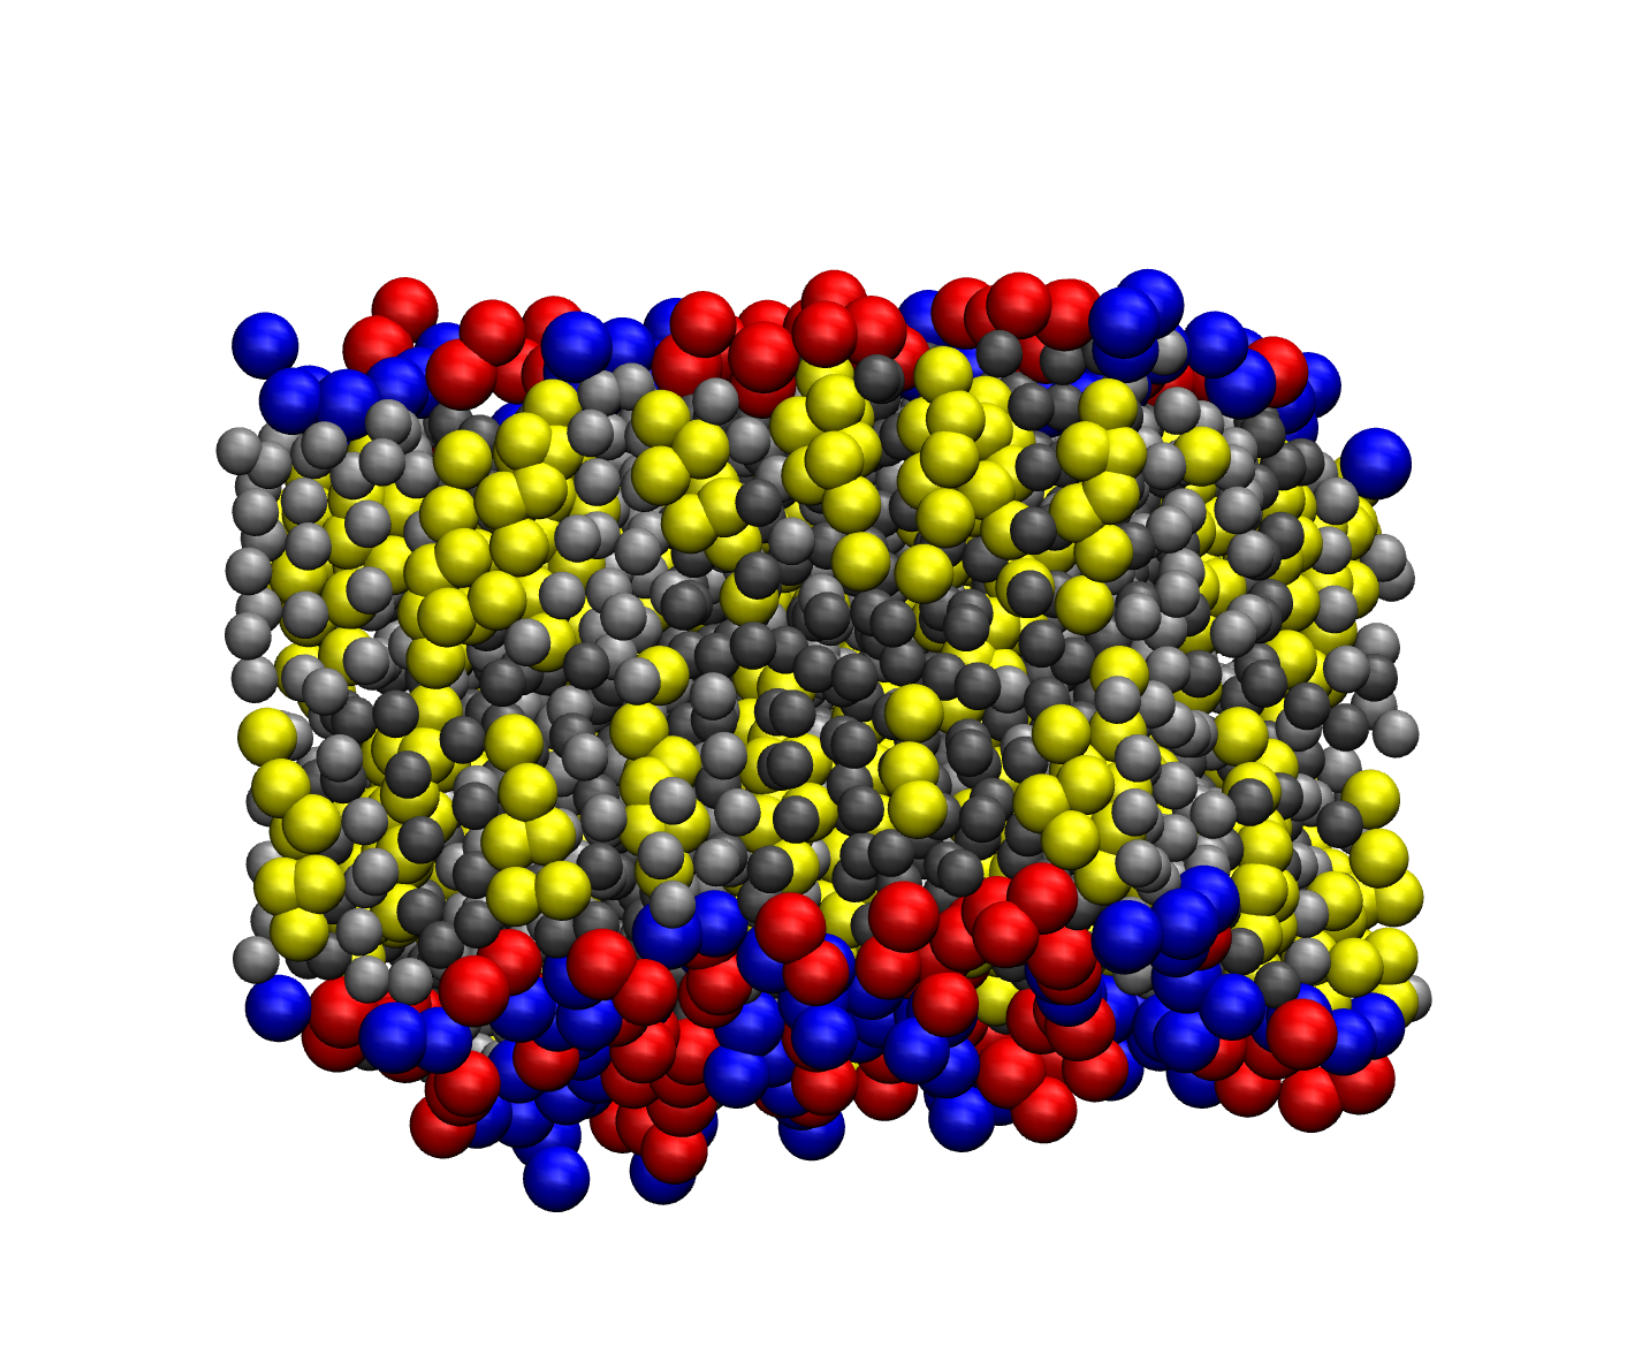
\includegraphics[width=\textwidth]{imagens/img1.jpg}
        \caption{Vista lateral}
    \end{subfigure}
    \hfill
    \begin{subfigure}[b]{0.24\textwidth}
        \centering
        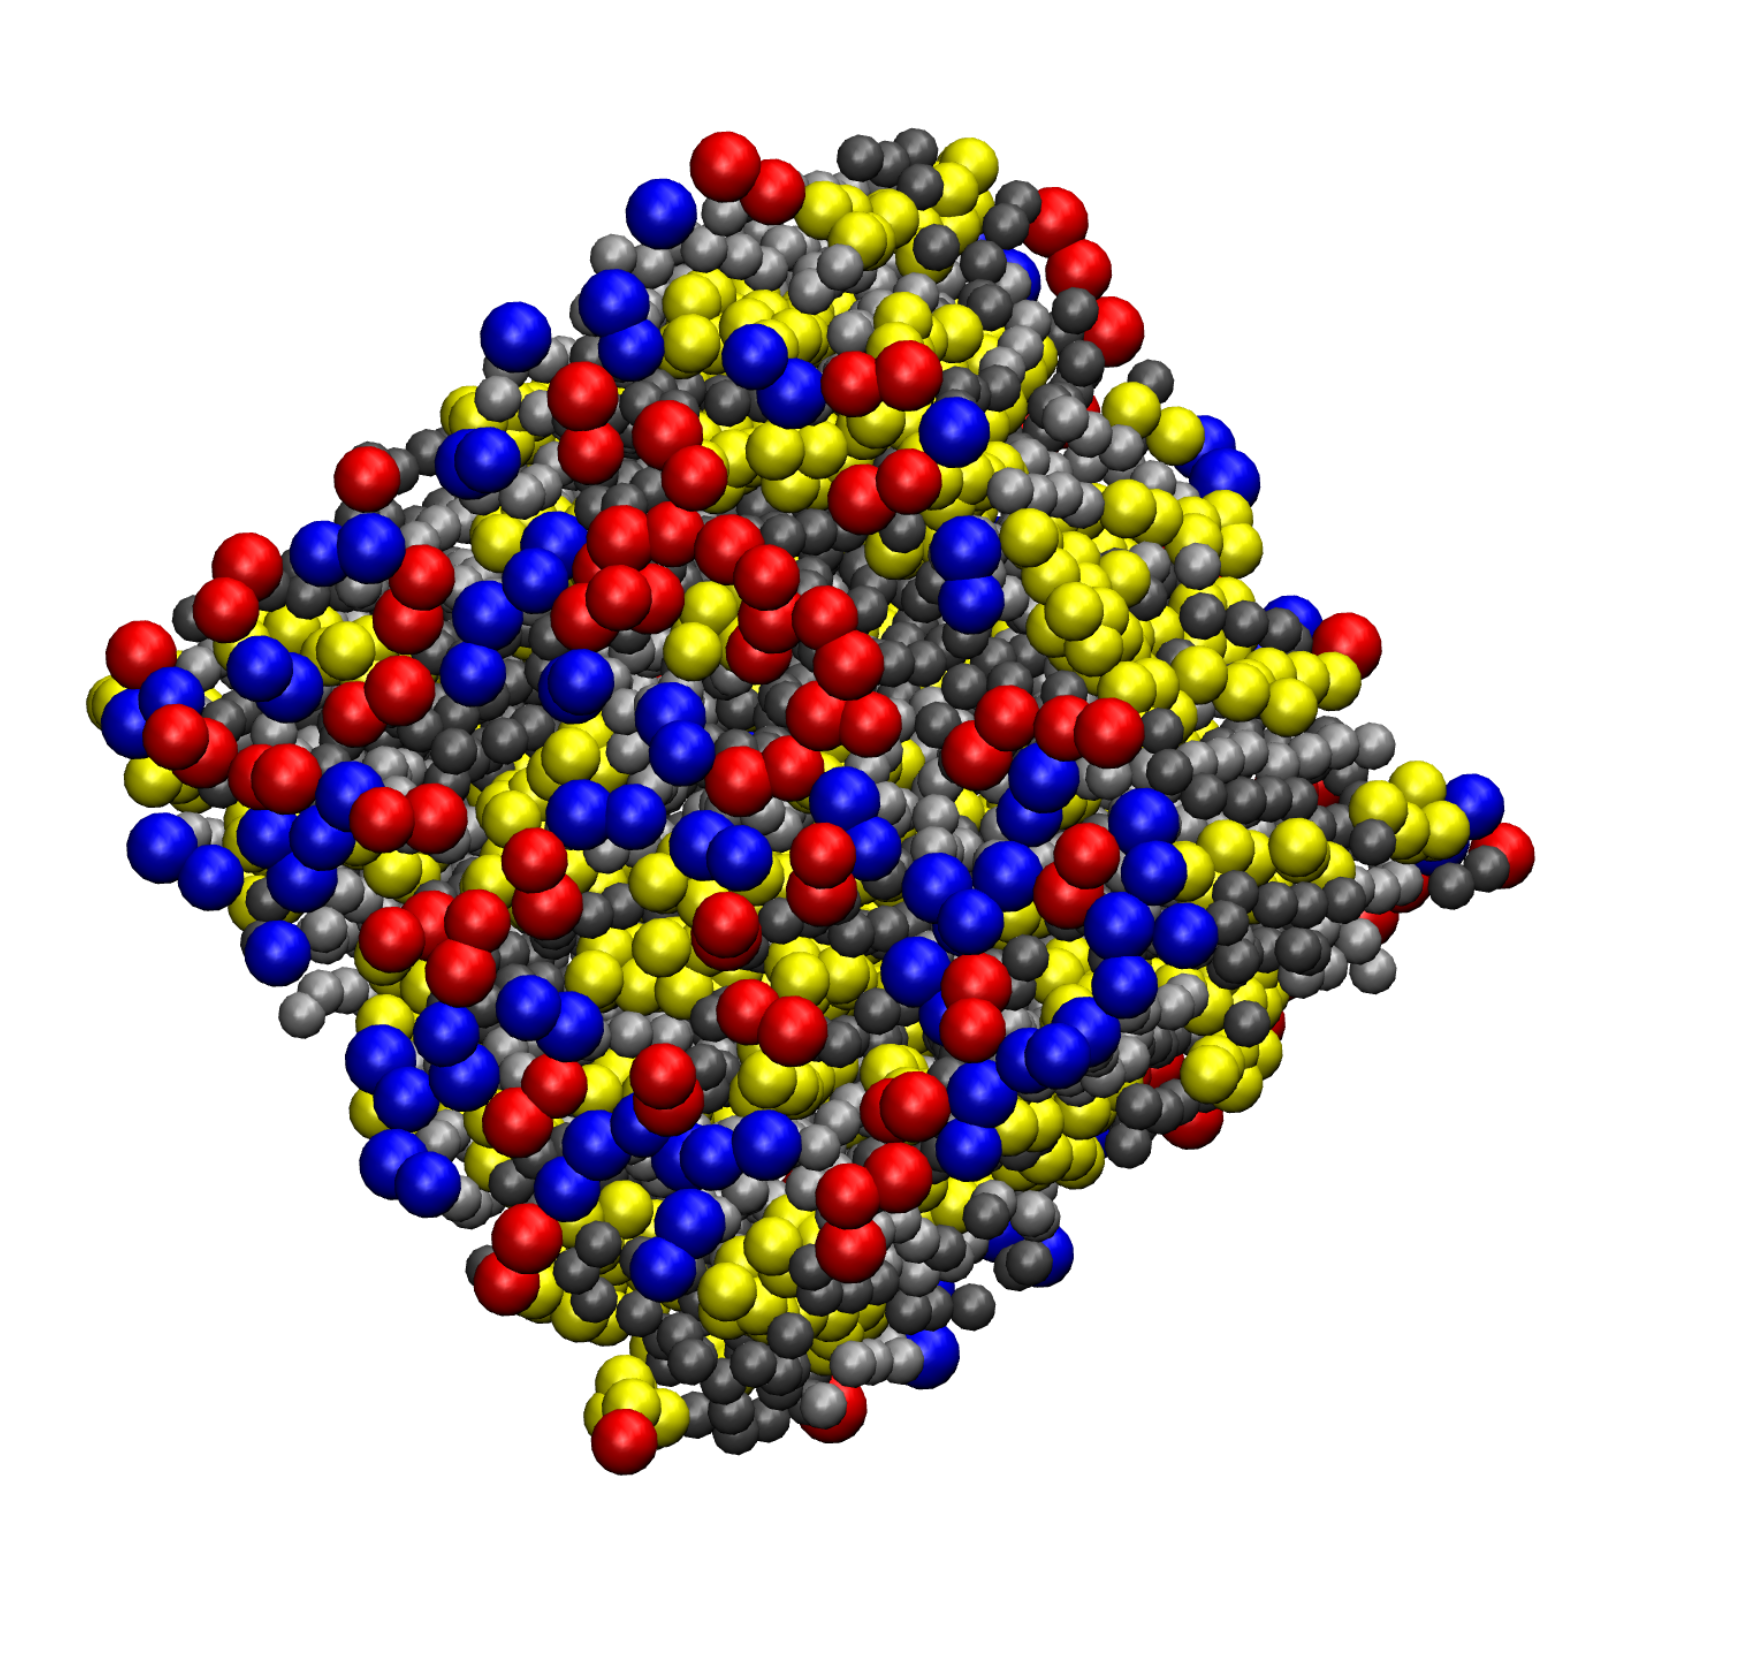
\includegraphics[width=\textwidth]{imagens/img3.jpg} 
        \caption{Frame $t_1$}
    \end{subfigure}
    \hfill
    \begin{subfigure}[b]{0.24\textwidth}
        \centering
        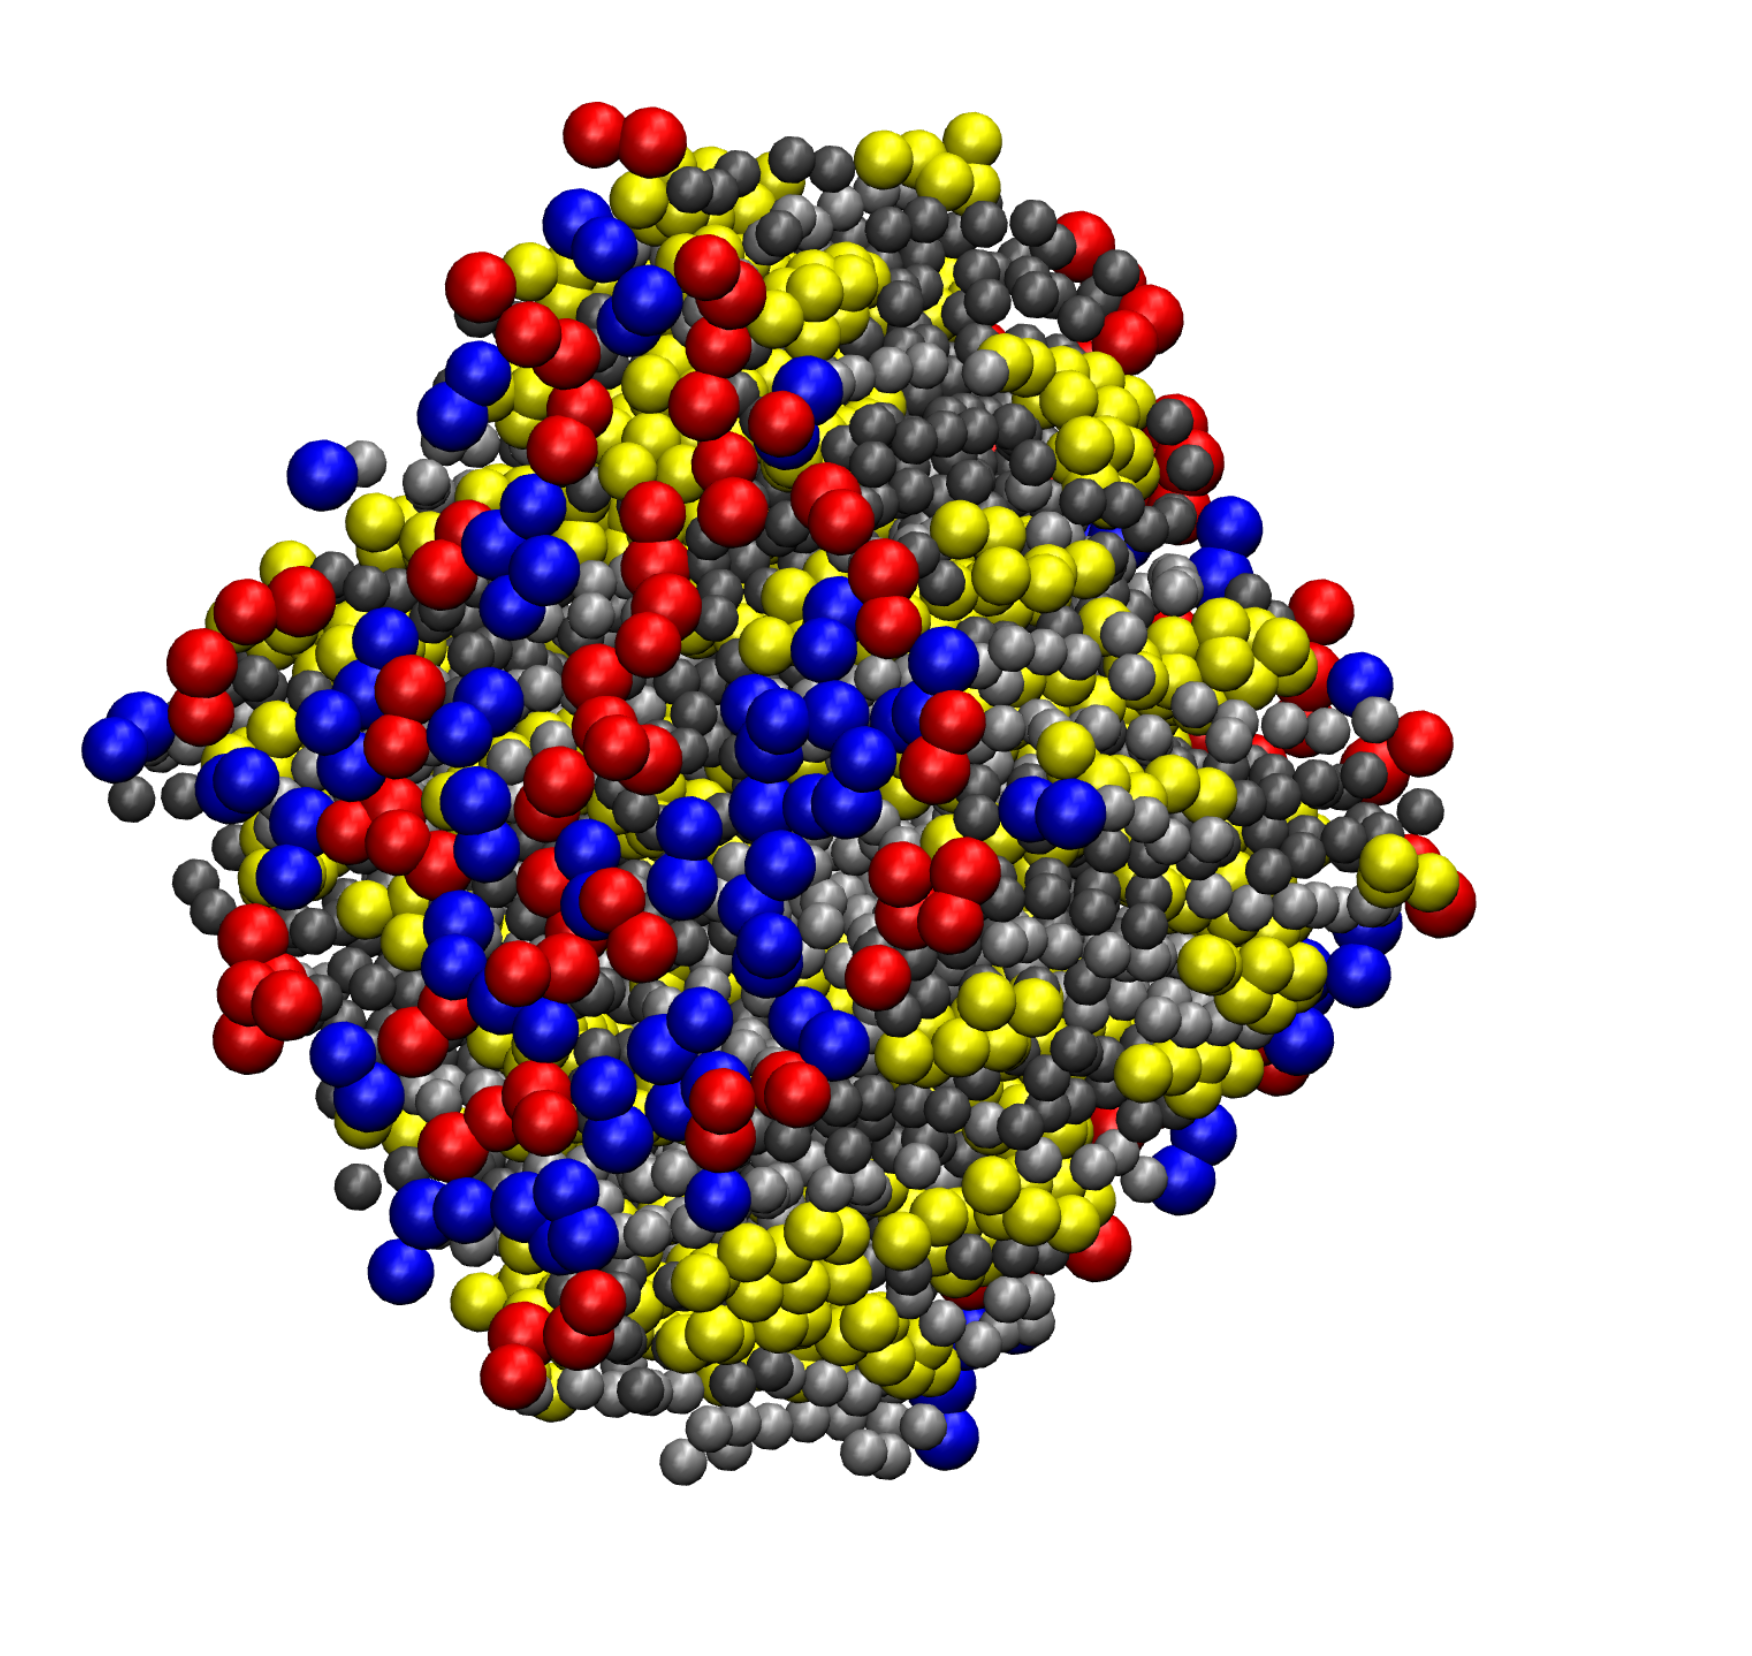
\includegraphics[width=\textwidth]{imagens/img4.jpg}
        \caption{Frame $t_2$}
    \end{subfigure}
    \hfill
    \begin{subfigure}[b]{0.24\textwidth}
        \centering
        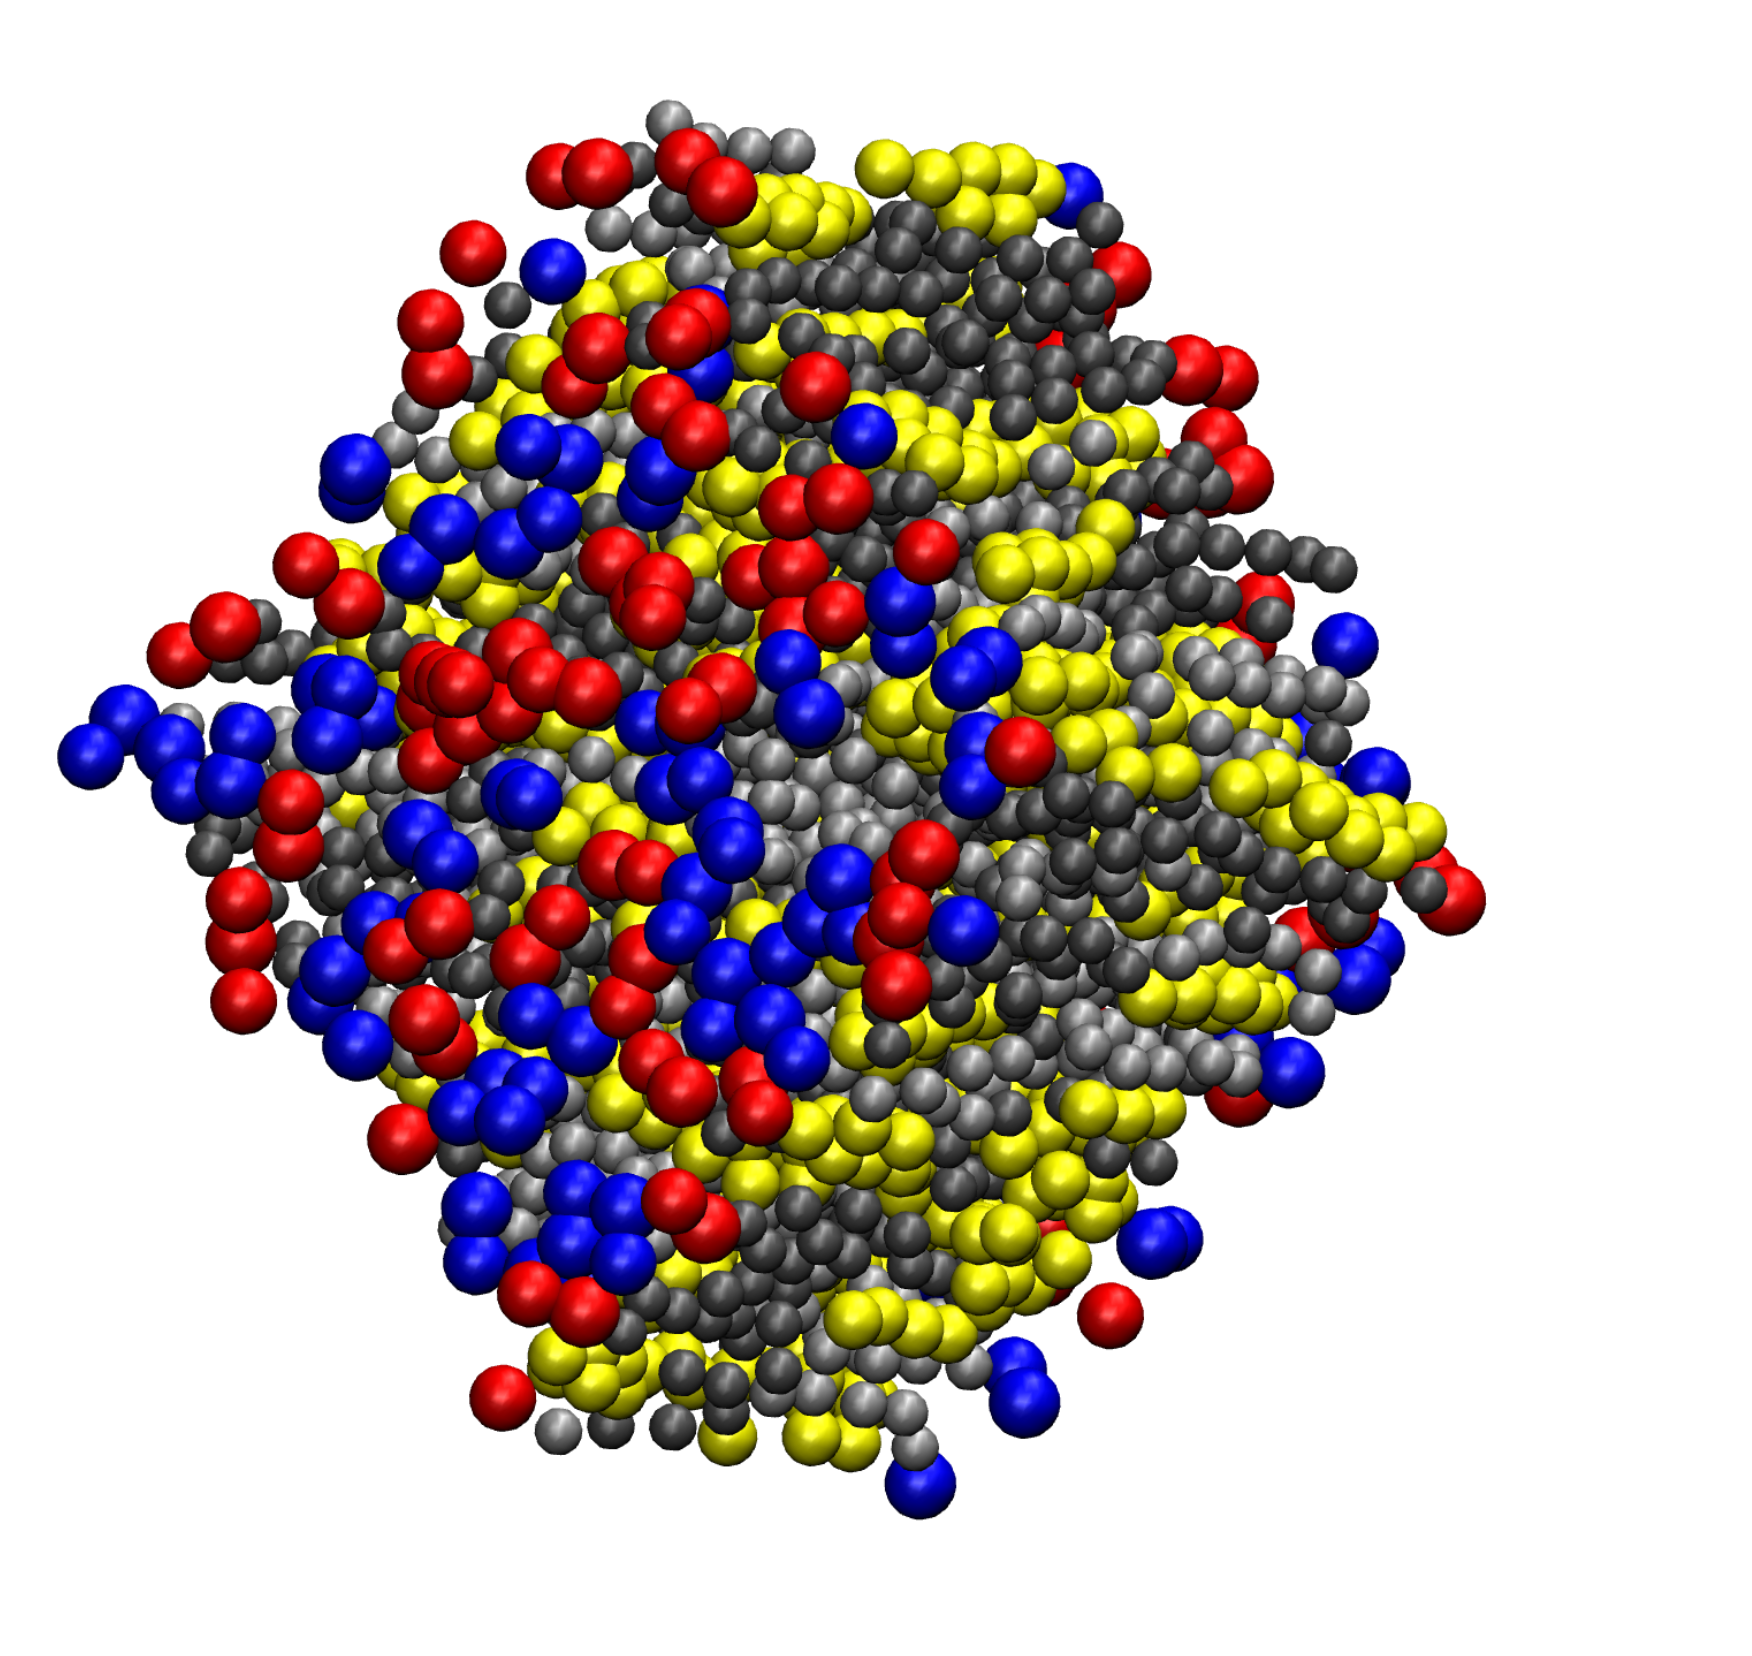
\includegraphics[width=\textwidth]{imagens/img5.jpg}
        \caption{Frame $t_3$}
    \end{subfigure}

    \vspace{0.4cm} 

    % ================= SEGUNDA LINHA (4 imagens) =================
    \begin{subfigure}[b]{0.24\textwidth}
        \centering
        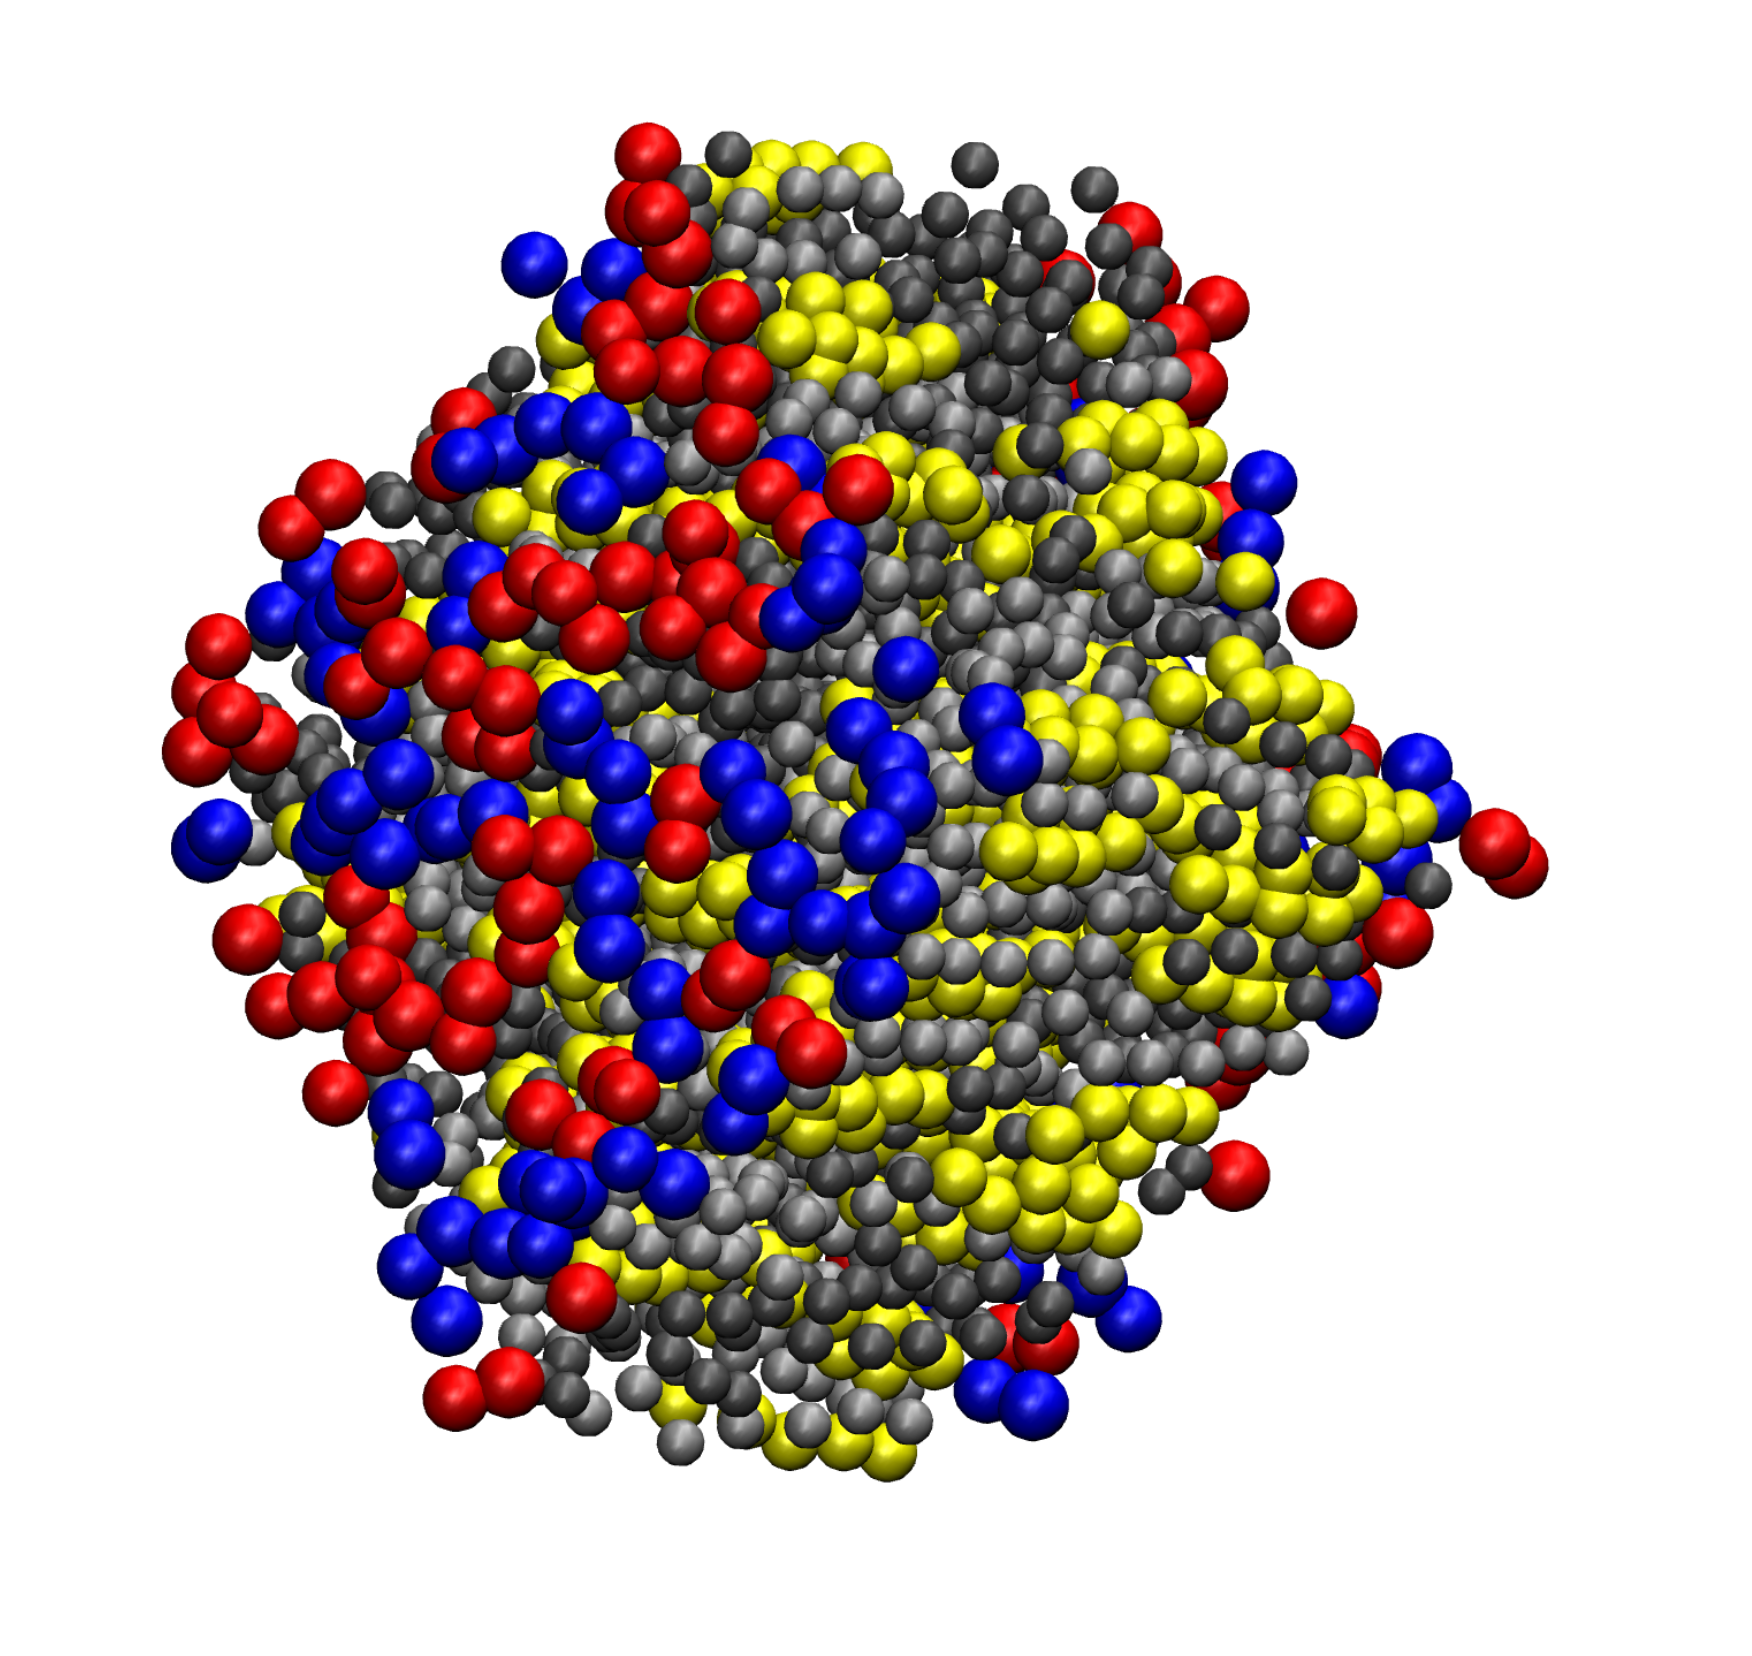
\includegraphics[width=\textwidth]{imagens/img6.jpg}
        \caption{Frame $t_4$}
    \end{subfigure}
    \hfill
    \begin{subfigure}[b]{0.24\textwidth}
        \centering
        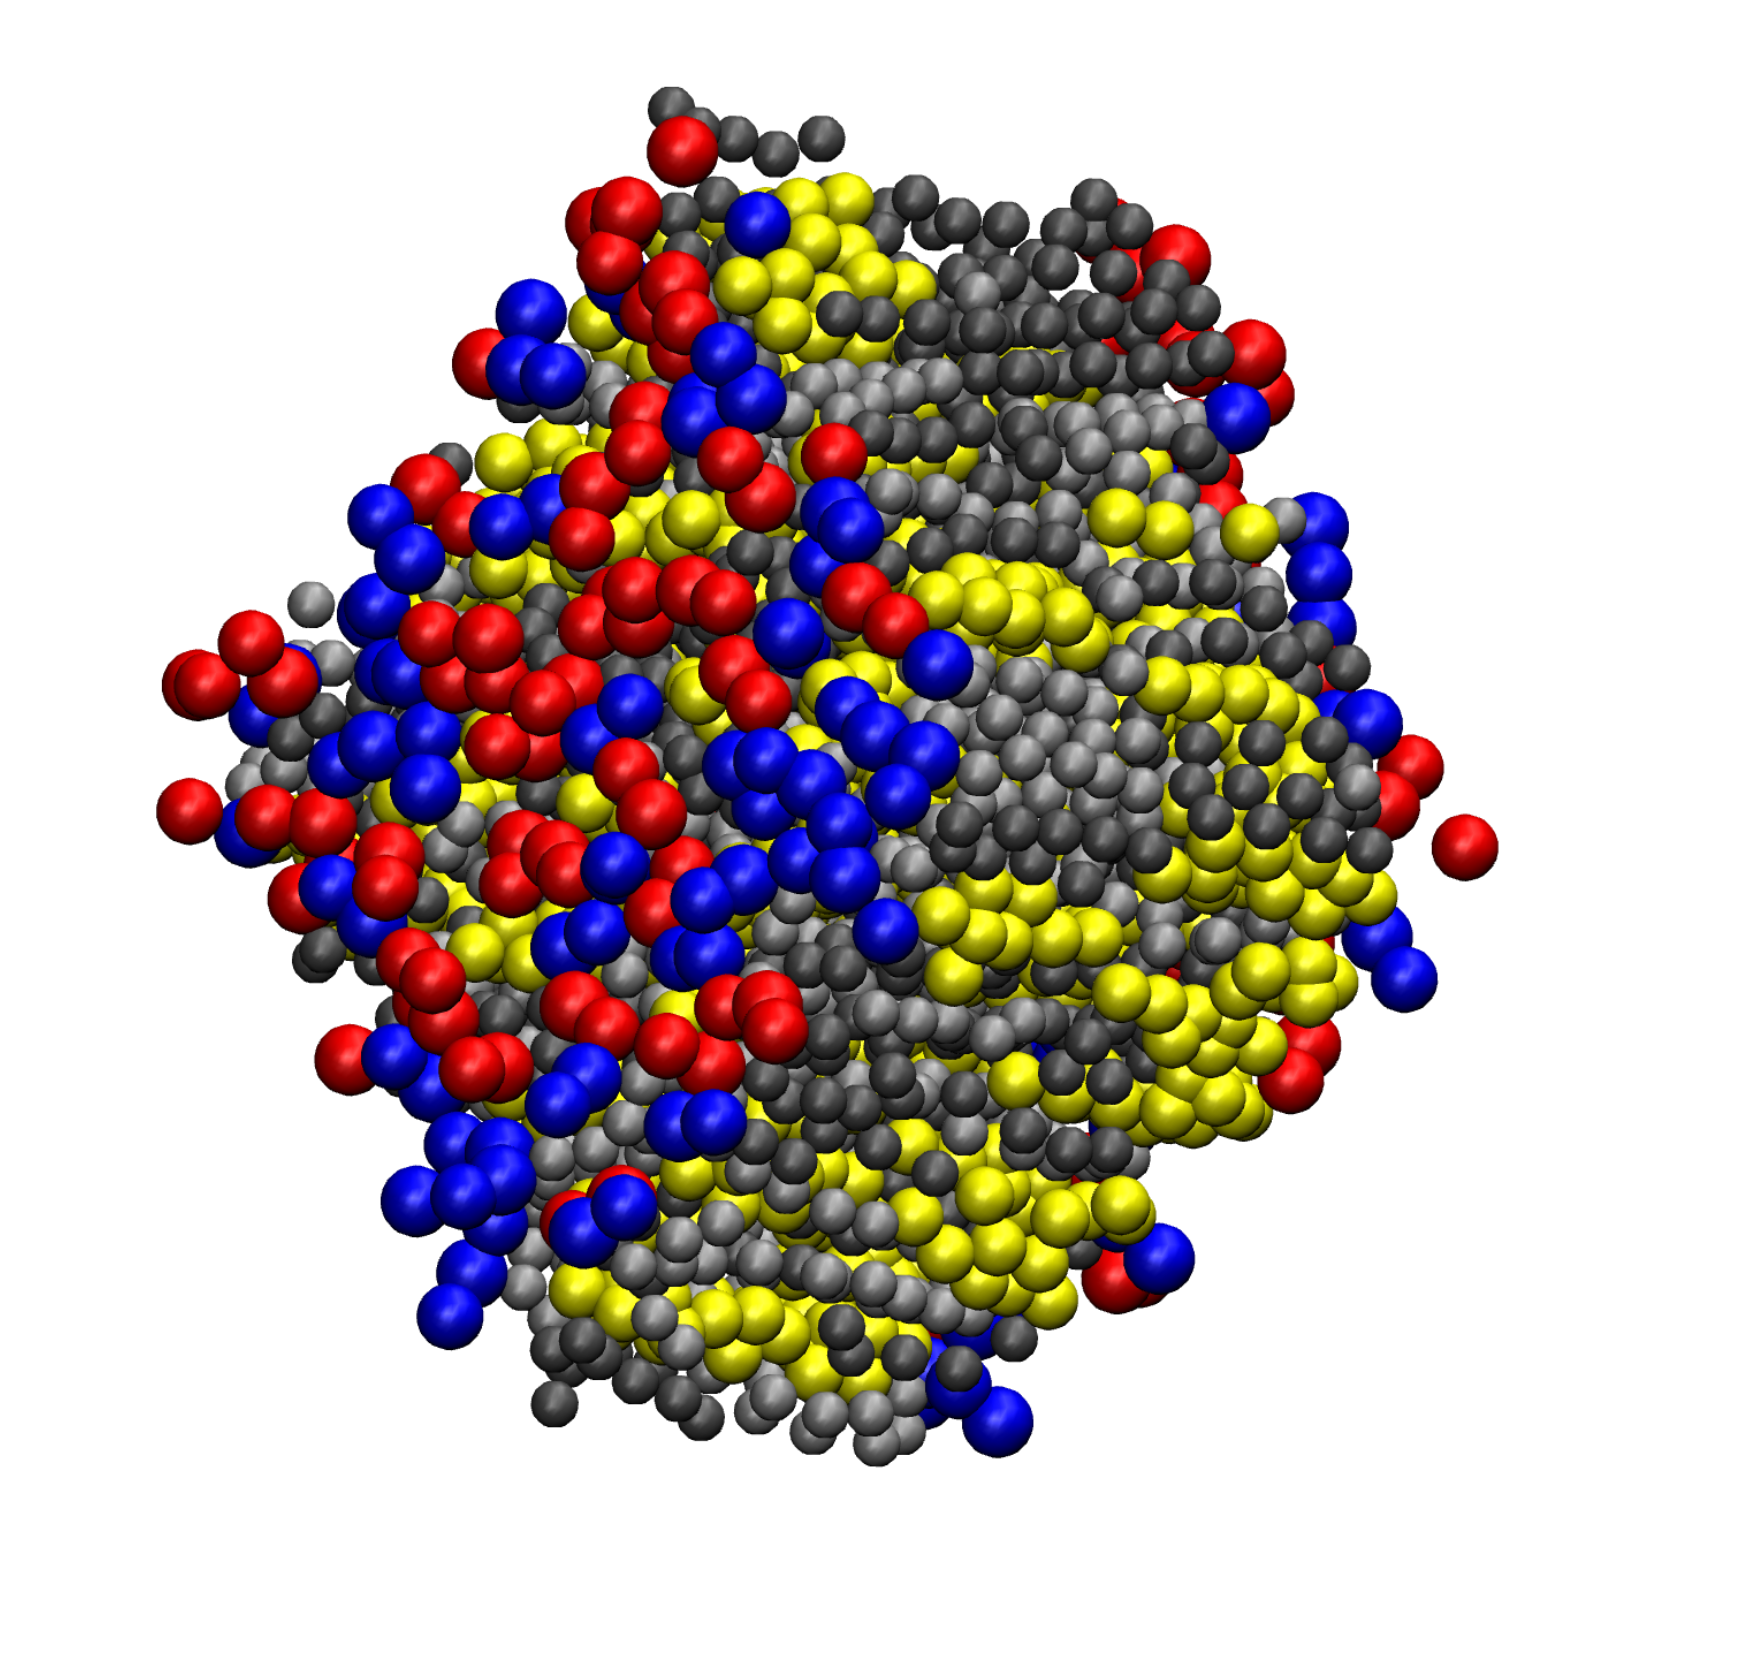
\includegraphics[width=\textwidth]{imagens/img7.jpg}
        \caption{Frame $t_5$}
    \end{subfigure}
    \hfill
    \begin{subfigure}[b]{0.24\textwidth}
        \centering
        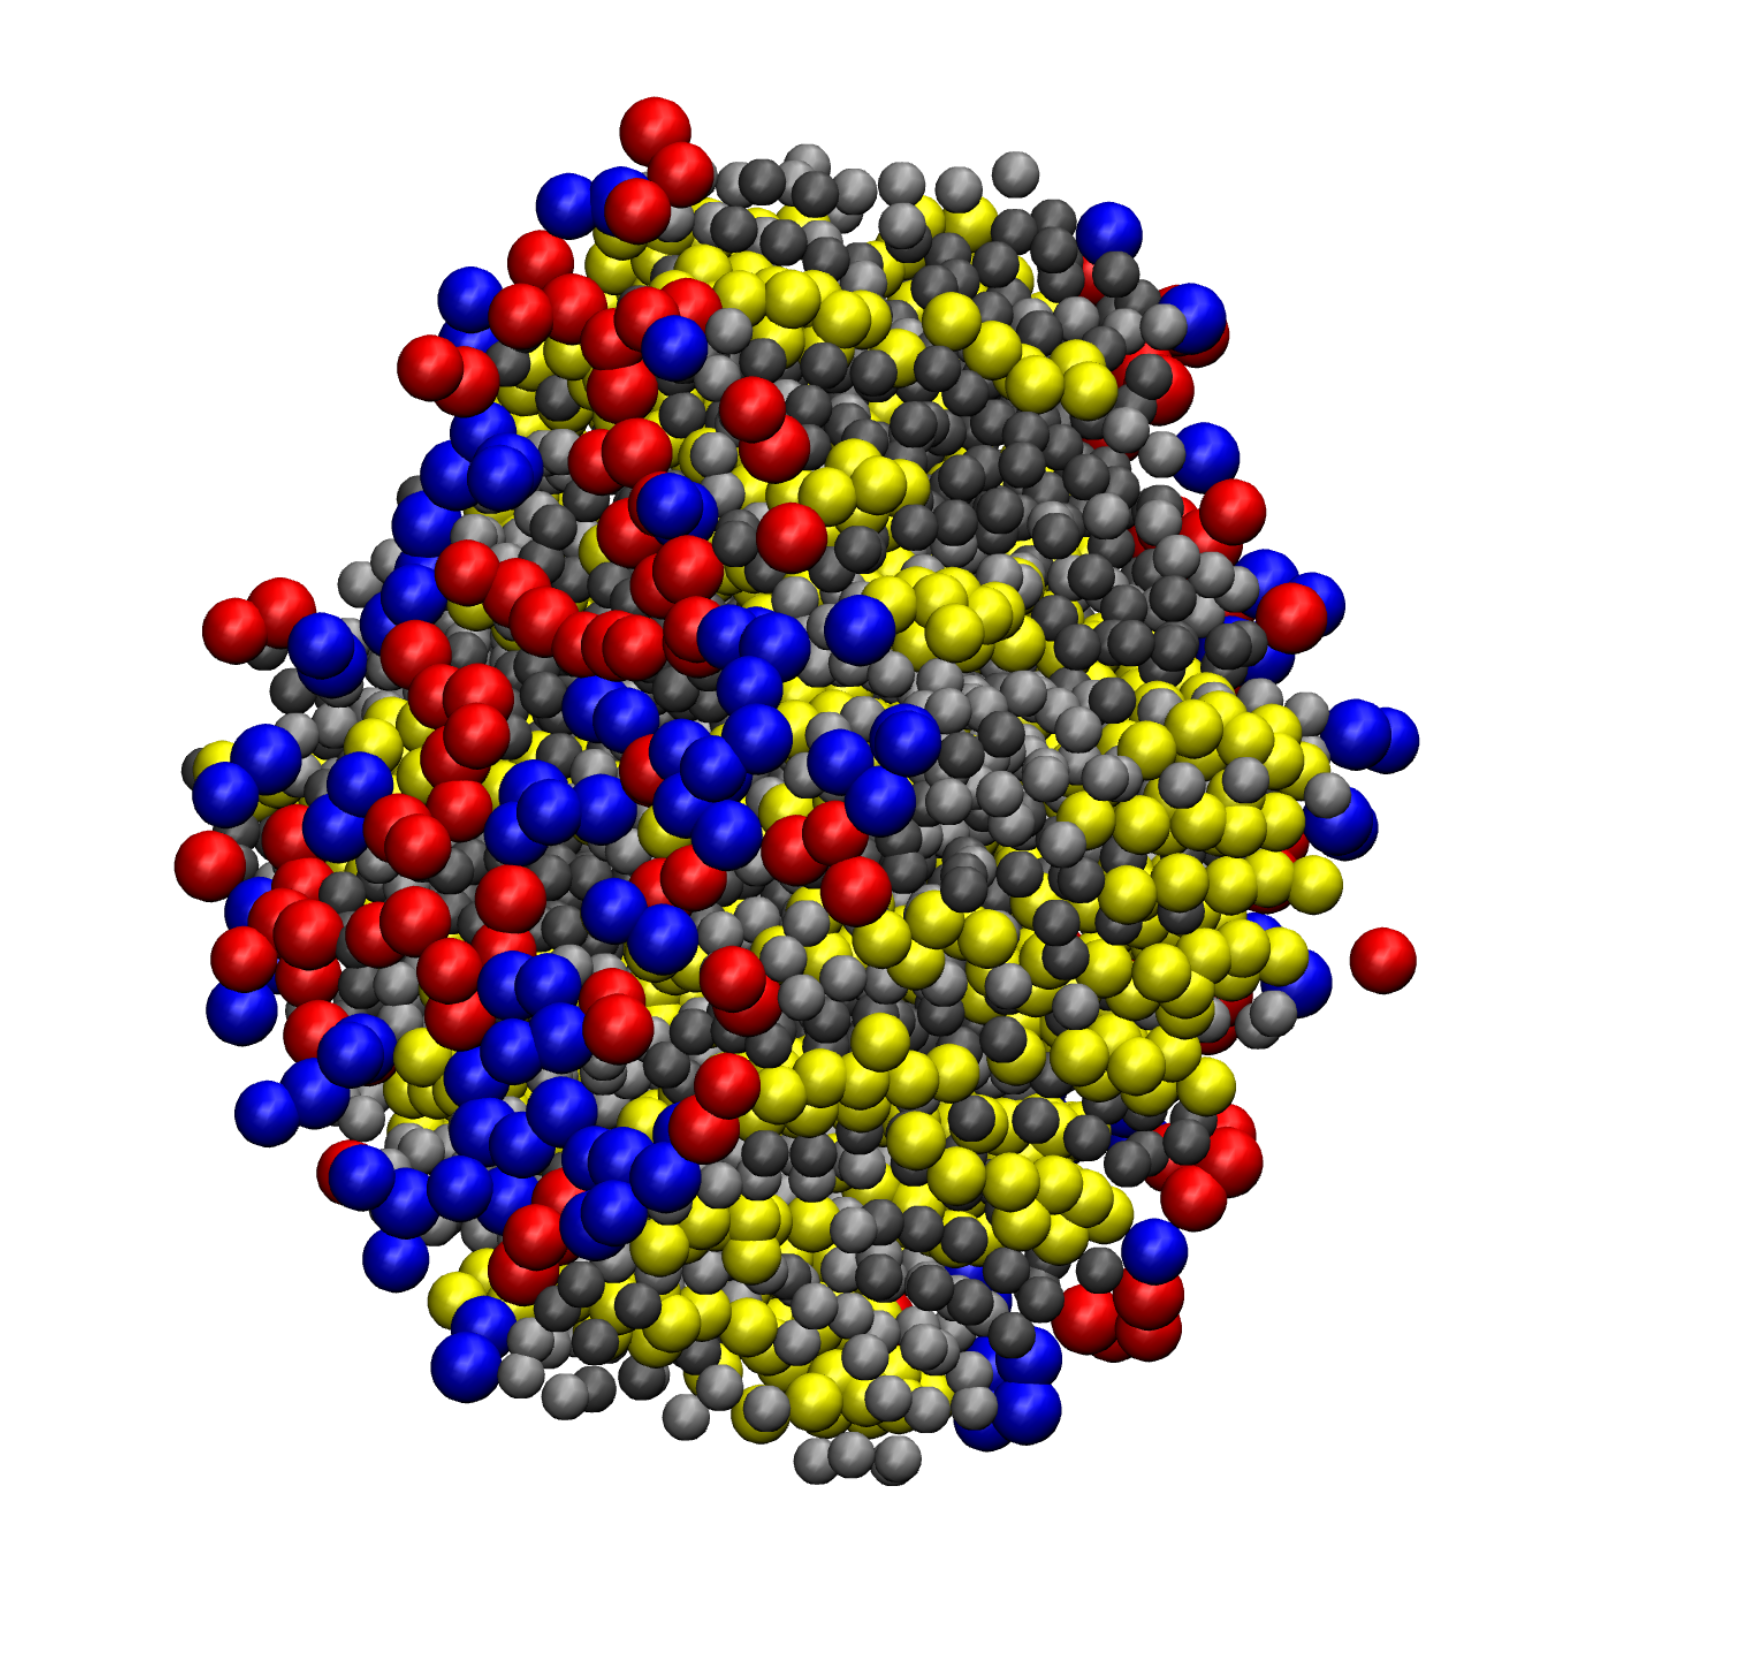
\includegraphics[width=\textwidth]{imagens/img8.jpg}
        \caption{Frame $t_6$}
    \end{subfigure}
    \hfill
    \begin{subfigure}[b]{0.24\textwidth}
        \centering
        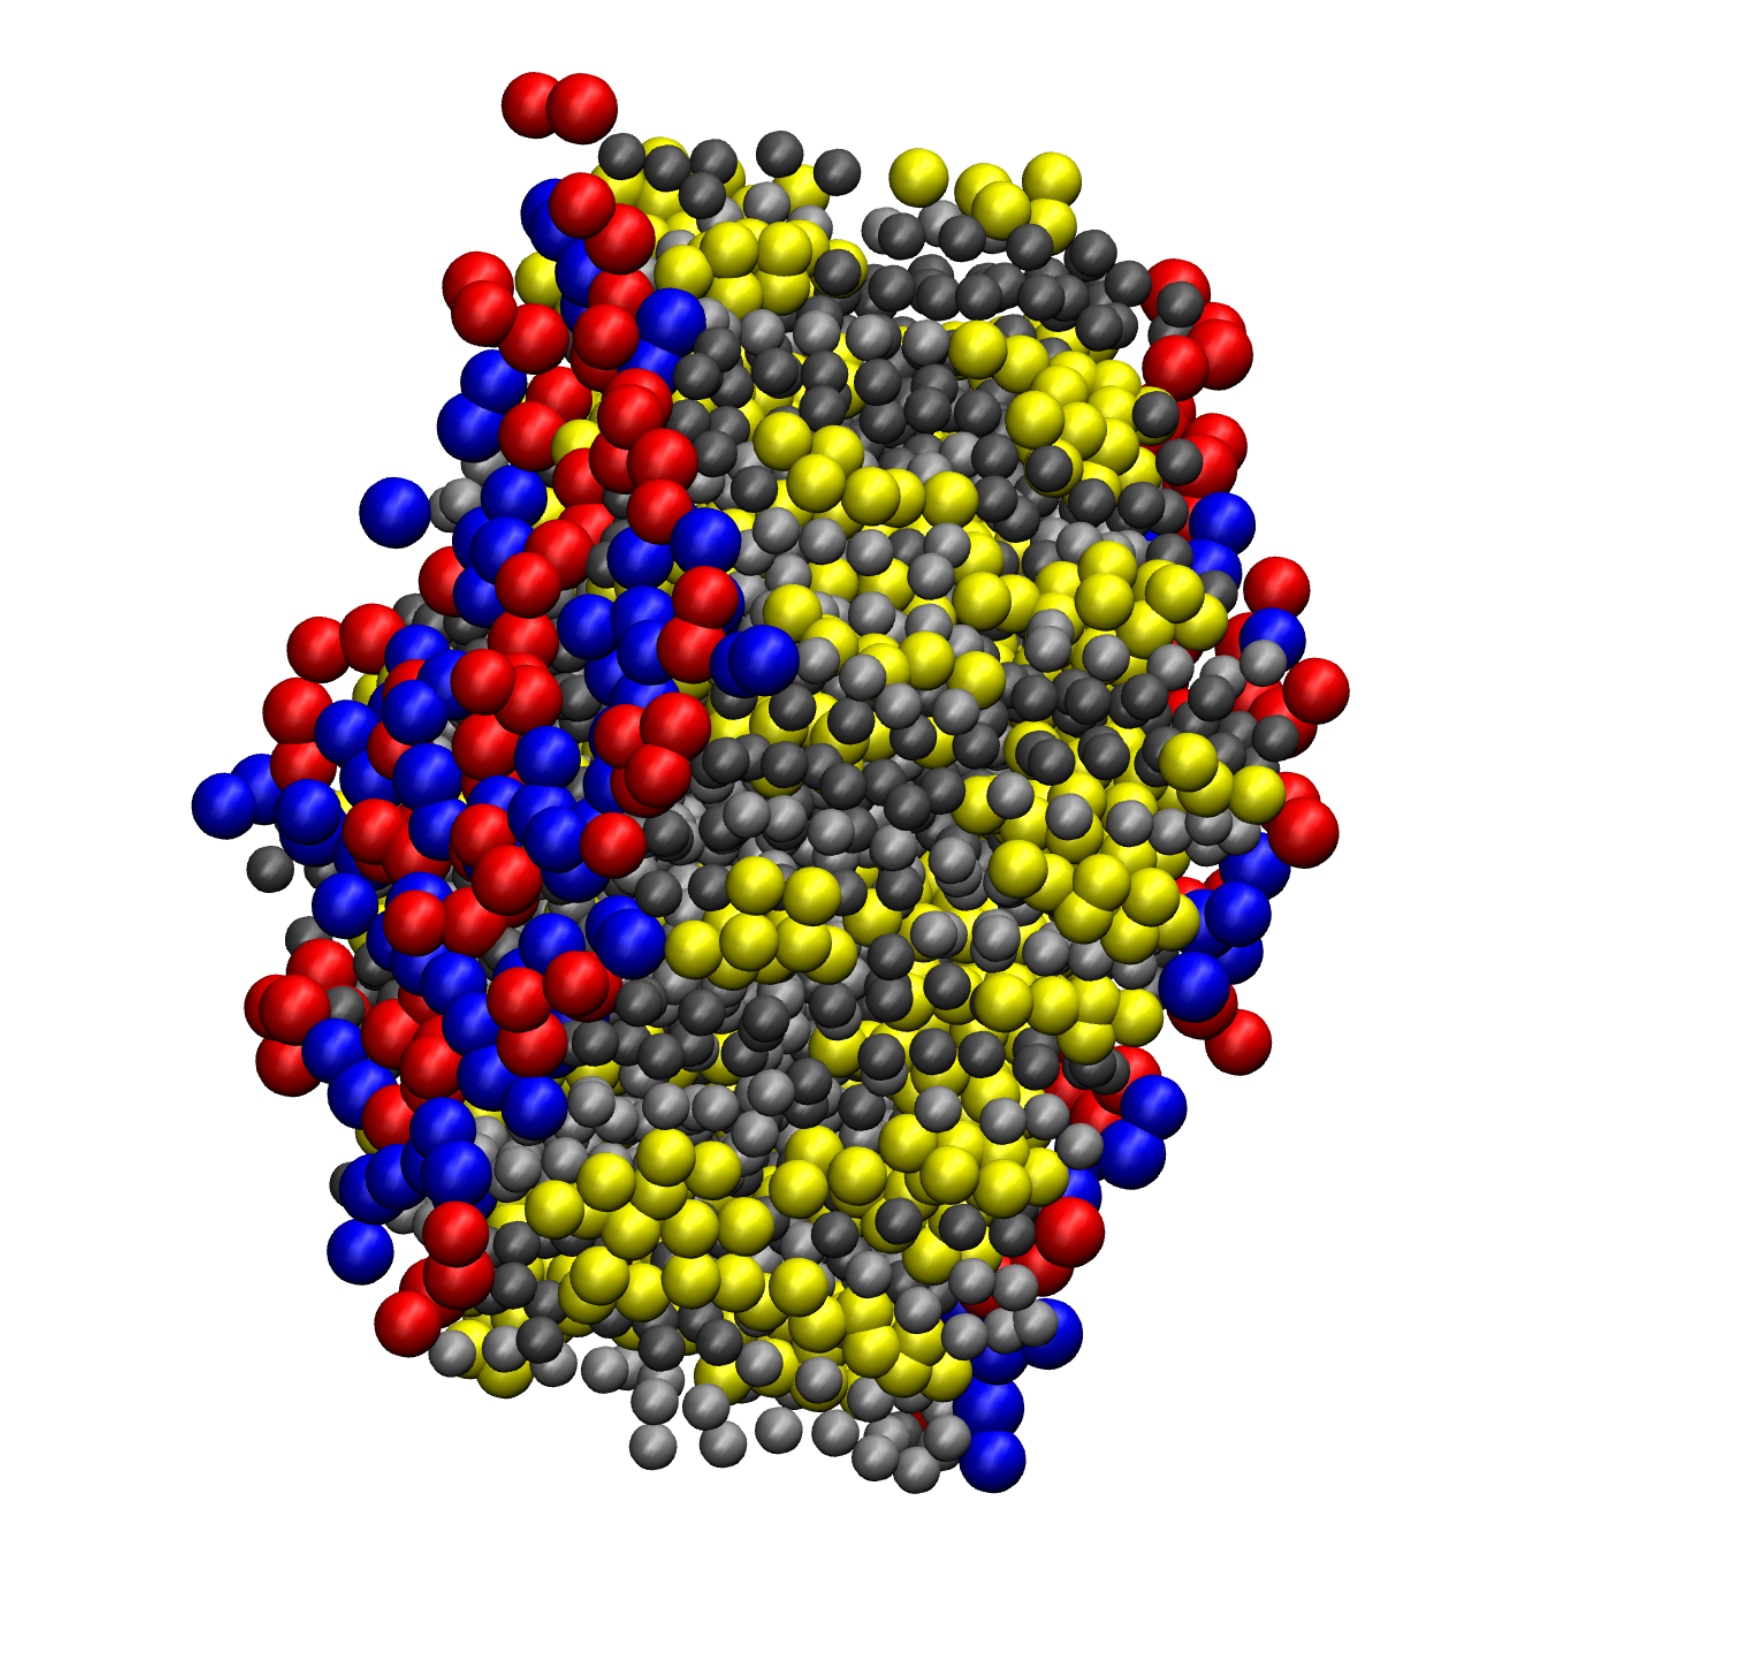
\includegraphics[width=\textwidth]{imagens/img9.jpg}
        \caption{Frame $t_7$}
    \end{subfigure}

    \caption{Mosaico do sistema DPPC/DSPC/Colesterol (40\% mol) a 333 K. Em (a), observa-se a vista lateral evidenciando o empacotamento das caudas. De (b) a (h), a evolução temporal confirma que a mistura se mantém estável, sem separação macroscópica de fases, com o colesterol (amarelo) dinamicamente intercalado e homogeneamente distribuído pelo núcleo hidrofóbico, sustentando a fase líquida-ordenada ($L_o$).}
    \label{fig:mosaico_dinamico}
\end{figure}

\subsubsection*{Perfil de Solvatação e Coordenação Iônica}

Para evidenciar a difusão dos eletrólitos na interface polar de forma analítica, optou-se por uma renderização com escala atômica ajustada. Ao atenuar os raios de van der Waals da malha hídrica e ampliar as sondas de sódio e cloreto, o mapeamento interfacial torna-se evidente sem obliterar o núcleo hidrofóbico (Figura \ref{fig:vmd_solvatacao}).

\begin{figure}[H]
    \centering
    % ================= TOPO: PANORÂMICA (Vista Lateral) =================
    \begin{subfigure}[b]{0.95\textwidth}
        \centering
        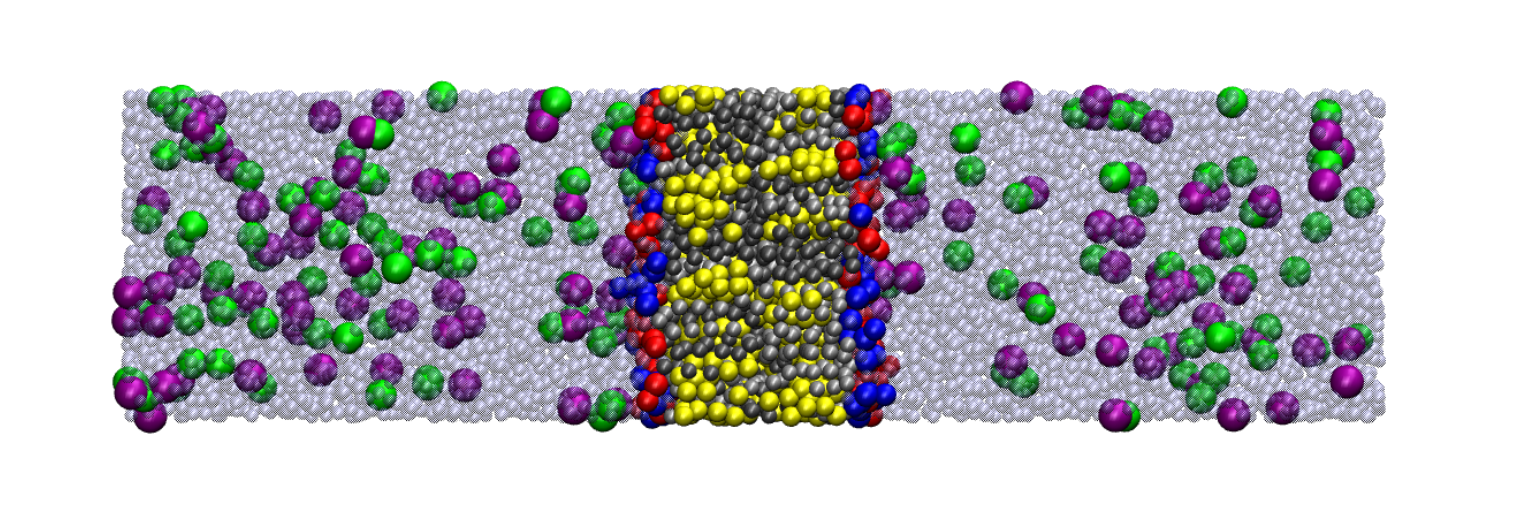
\includegraphics[width=\textwidth]{imagens/img_panoramica_140505.png} 
        \caption{Corte transversal evidenciando a completa solvatação da bicamada}
    \end{subfigure}

    \vspace{0.6cm} 

    % ================= BASE: 3 PERSPECTIVAS LADO A LADO =================
    \begin{subfigure}[b]{0.31\textwidth}
        \centering
        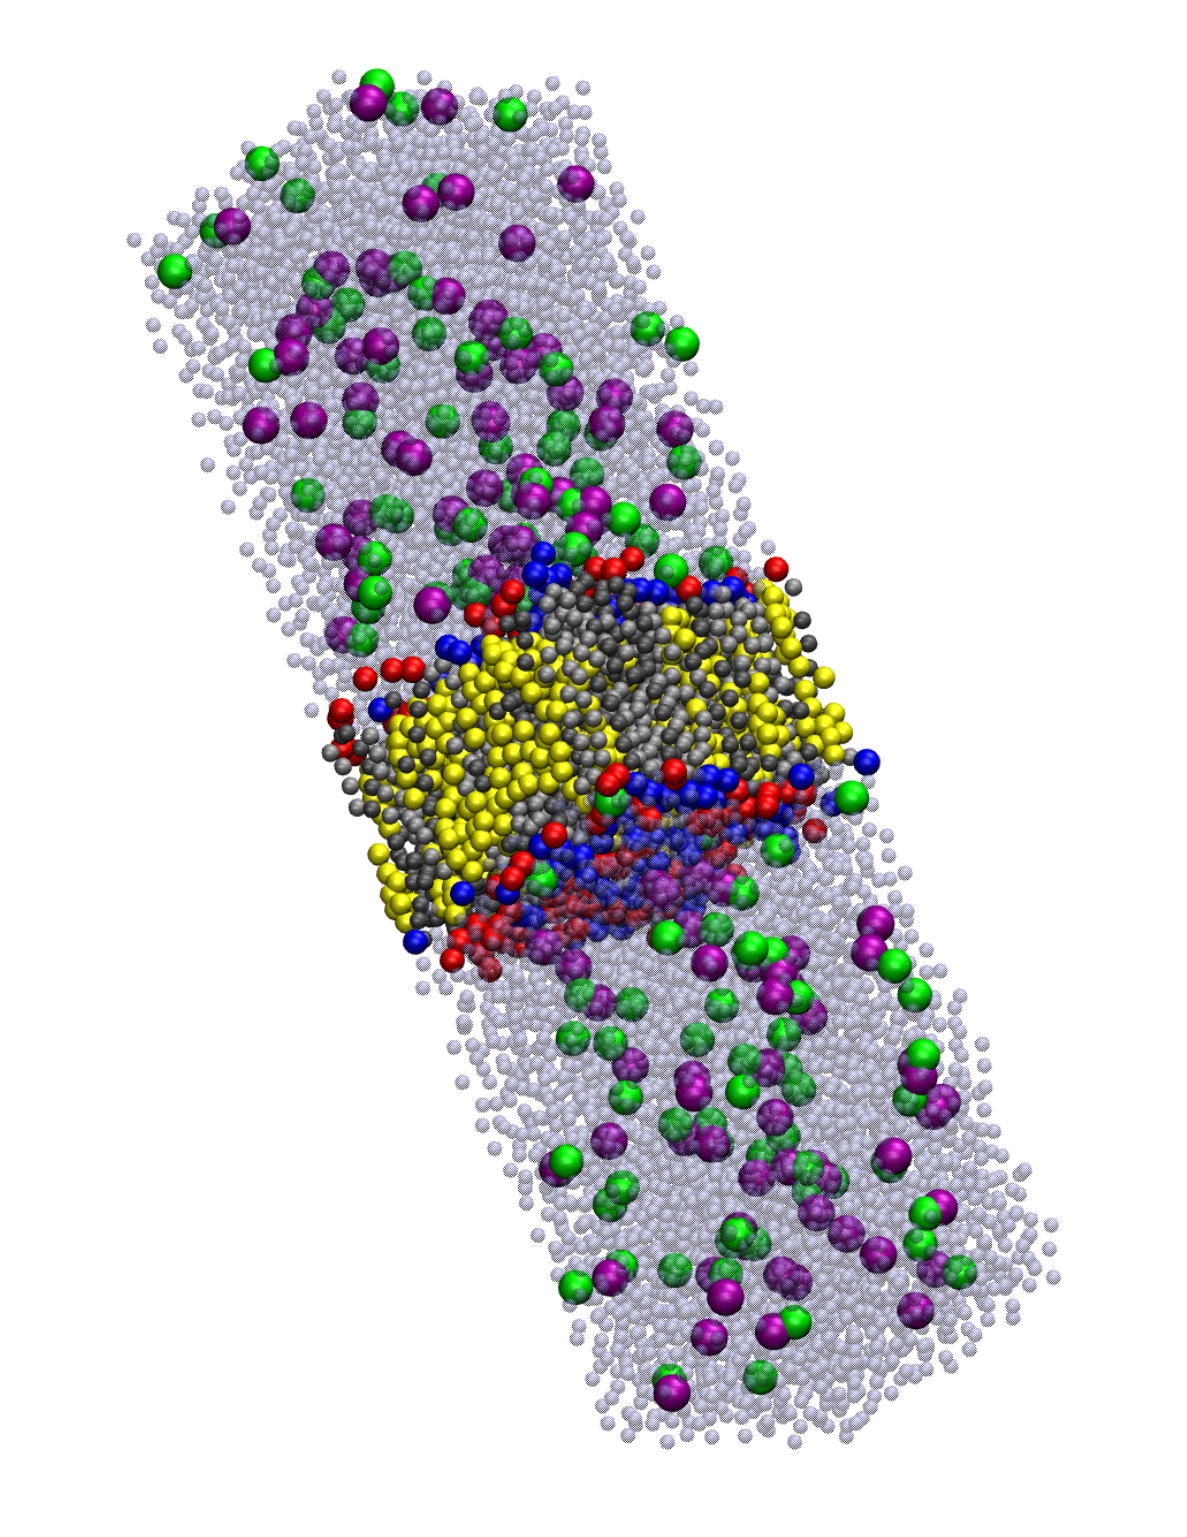
\includegraphics[width=\textwidth]{imagens/img_persp_135957.png} 
        \caption{Vista isométrica A}
    \end{subfigure}
    \hfill
    \begin{subfigure}[b]{0.31\textwidth}
        \centering
        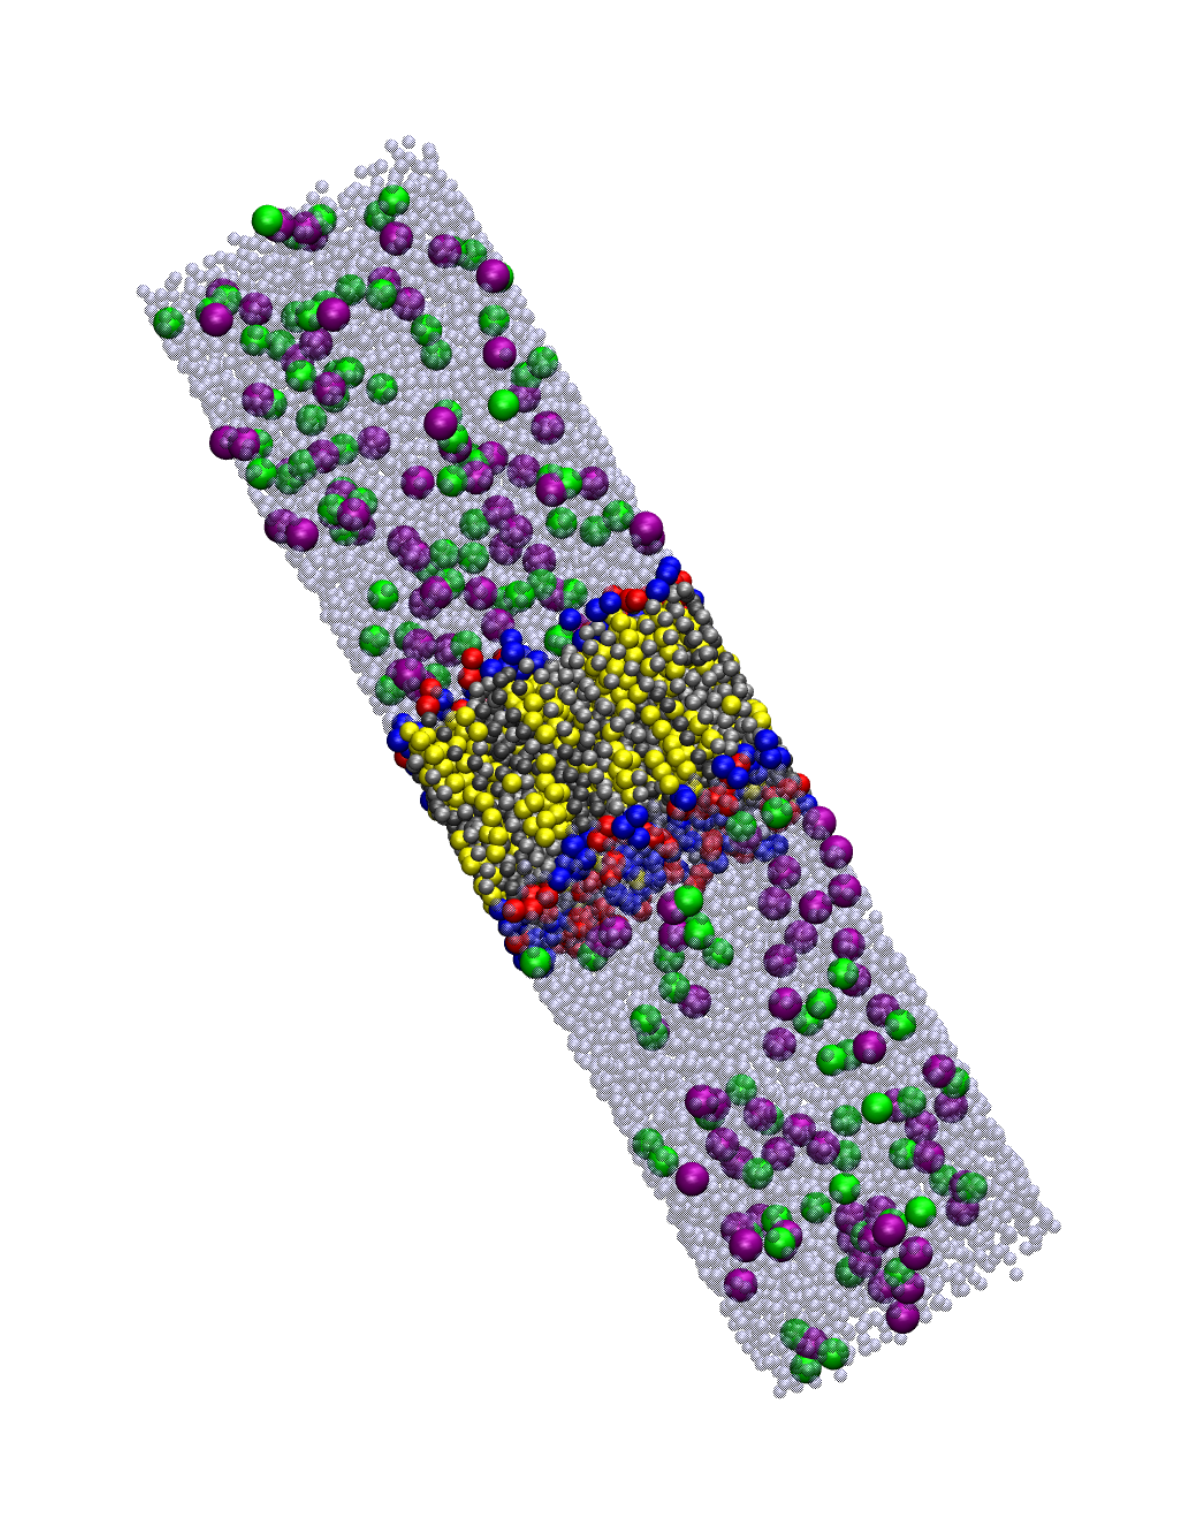
\includegraphics[width=\textwidth]{imagens/img_persp_140217.png} 
        \caption{Vista isométrica B}
    \end{subfigure}
    \hfill
    \begin{subfigure}[b]{0.31\textwidth}
        \centering
        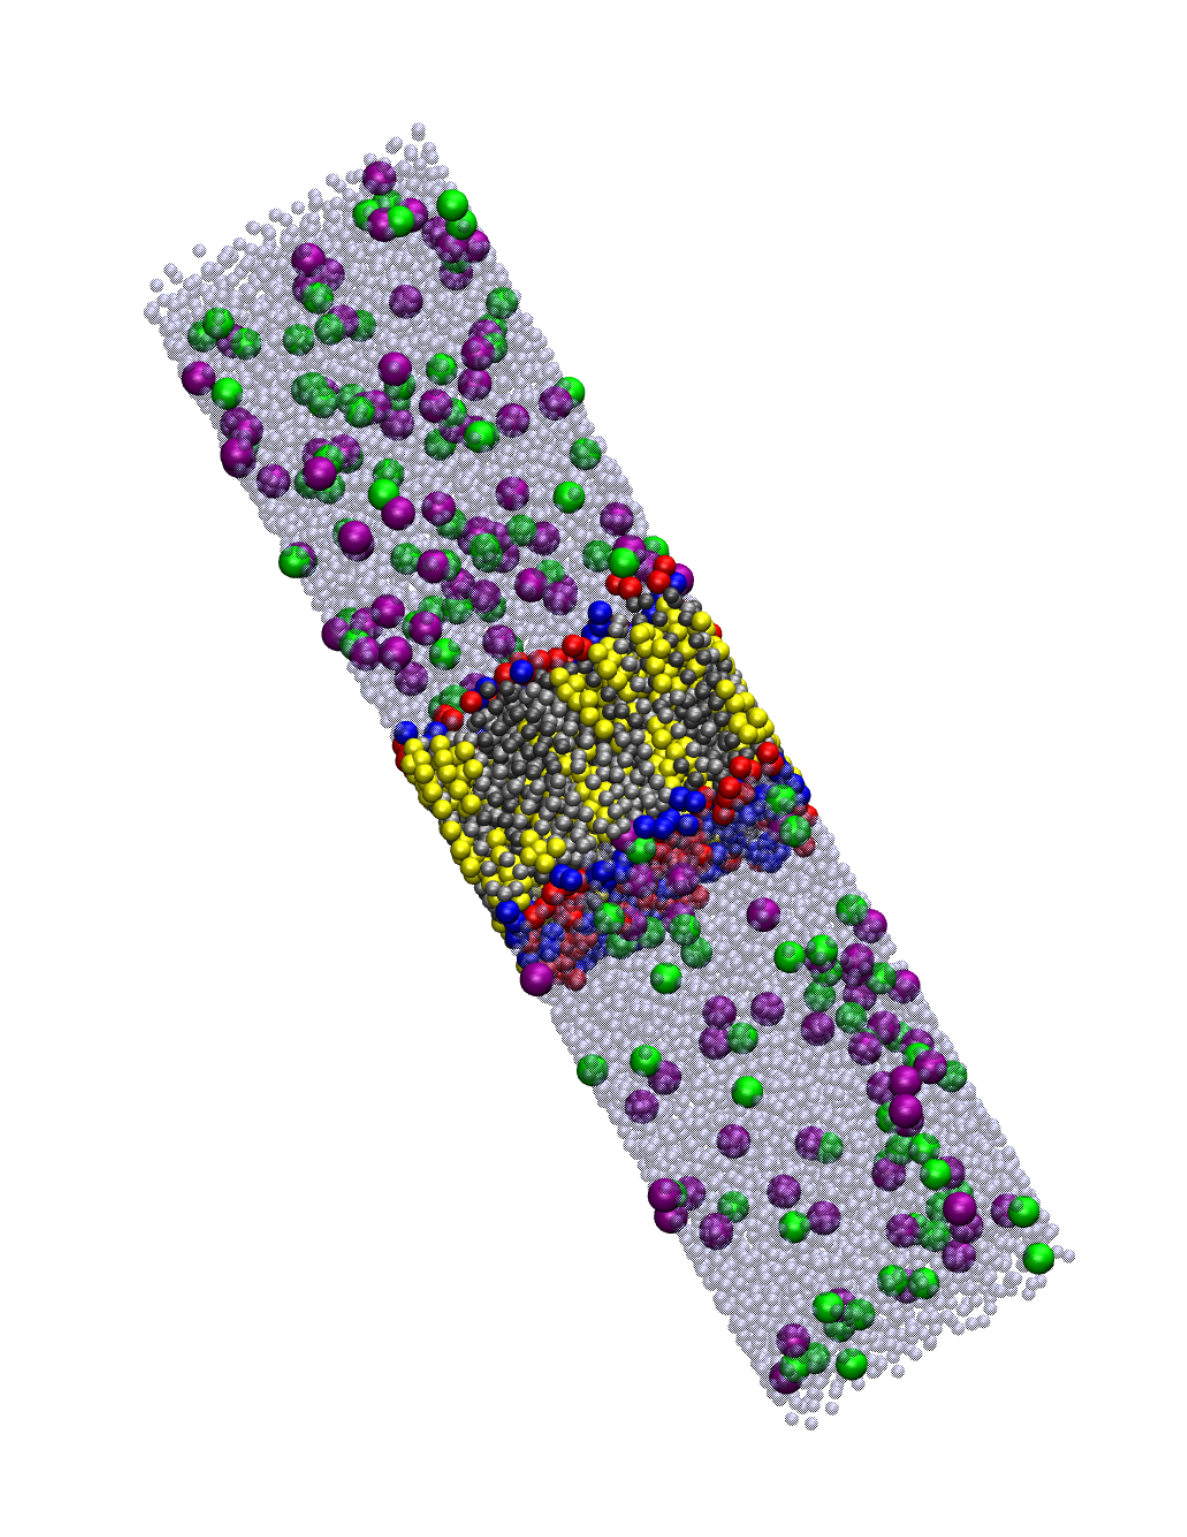
\includegraphics[width=\textwidth]{imagens/img_persp_140322.png} 
        \caption{Vista isométrica C}
    \end{subfigure}

    \caption{Visualização da solvatação e distribuição iônica do sistema DPPC/DSPC/Colesterol em meio salino a 333 K. Para fins de clareza analítica, utilizou-se uma escala atômica modificada: a malha de água (esferas azuis translúcidas) apresenta raio reduzido, enquanto os íons de Na$^+$ (verde) e Cl$^-$ (roxo) encontram-se ampliados, destacando a sua distribuição volumétrica na fase aquosa e a ausência de permeação no núcleo hidrofóbico denso ($L_o$).}
    \label{fig:vmd_solvatacao}
\end{figure}

\subsubsection*{Mismatch Hidrofóbico e Acomodação Interfacial}

A resposta topológica da membrana à disparidade do comprimento das cadeias acílicas (\textit{hydrophobic mismatch}) encontra-se ilustrada na Figura \ref{fig:mosaico_mismatch}. O comparativo visual espelha o ganho de espessura transversal e as alterações na distribuição geométrica da solvatação discutidas nas análises termodinâmicas anteriores.

\begin{figure}[H]
    \centering
    % ================= LINHA 1: Vistas Laterais =================
    \begin{subfigure}[b]{0.26\textwidth}
        \centering
        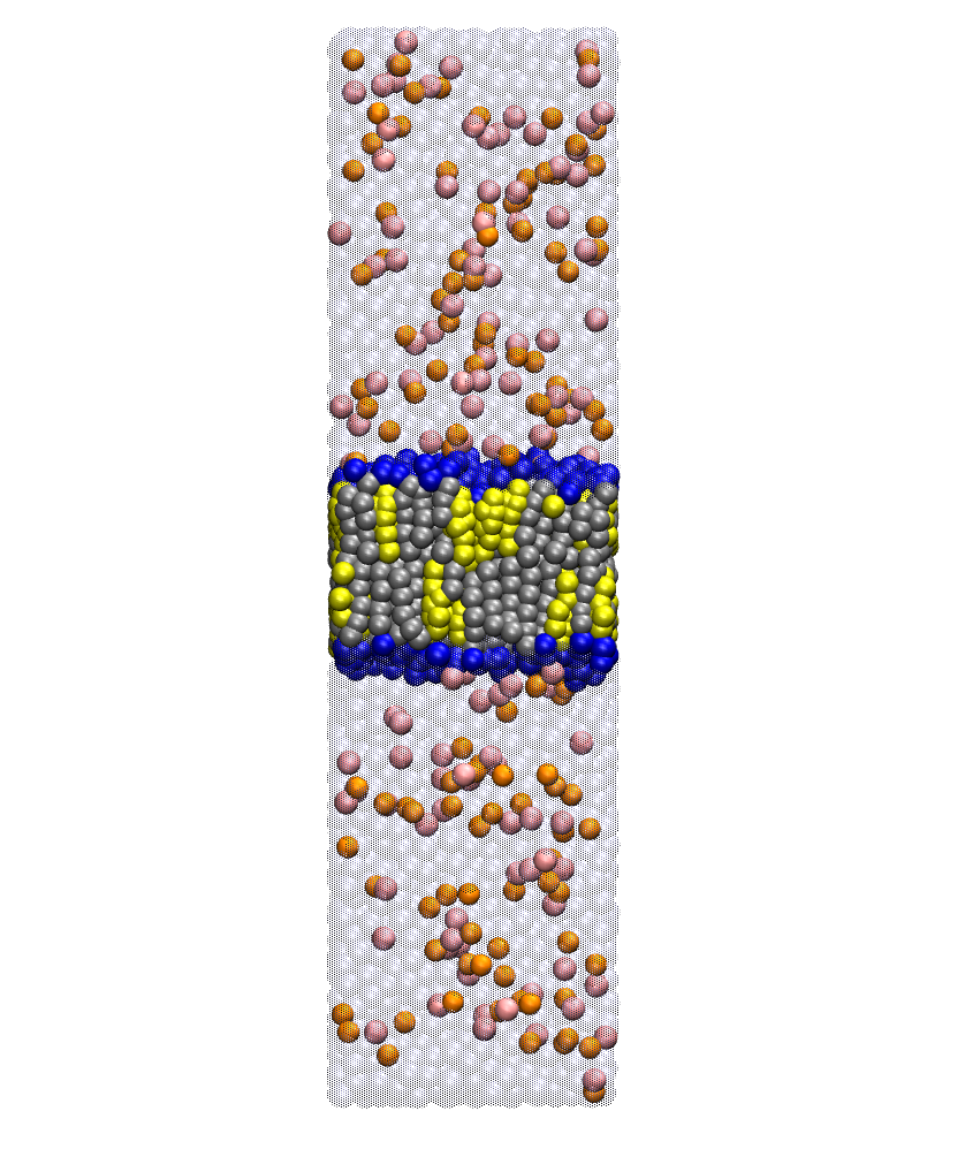
\includegraphics[width=\textwidth]{imagens/dppc_lat.png}
        \caption{DPPC (C16) - Vista Lateral}
    \end{subfigure}
    \hspace{1.5cm} 
    \begin{subfigure}[b]{0.26\textwidth}
        \centering
        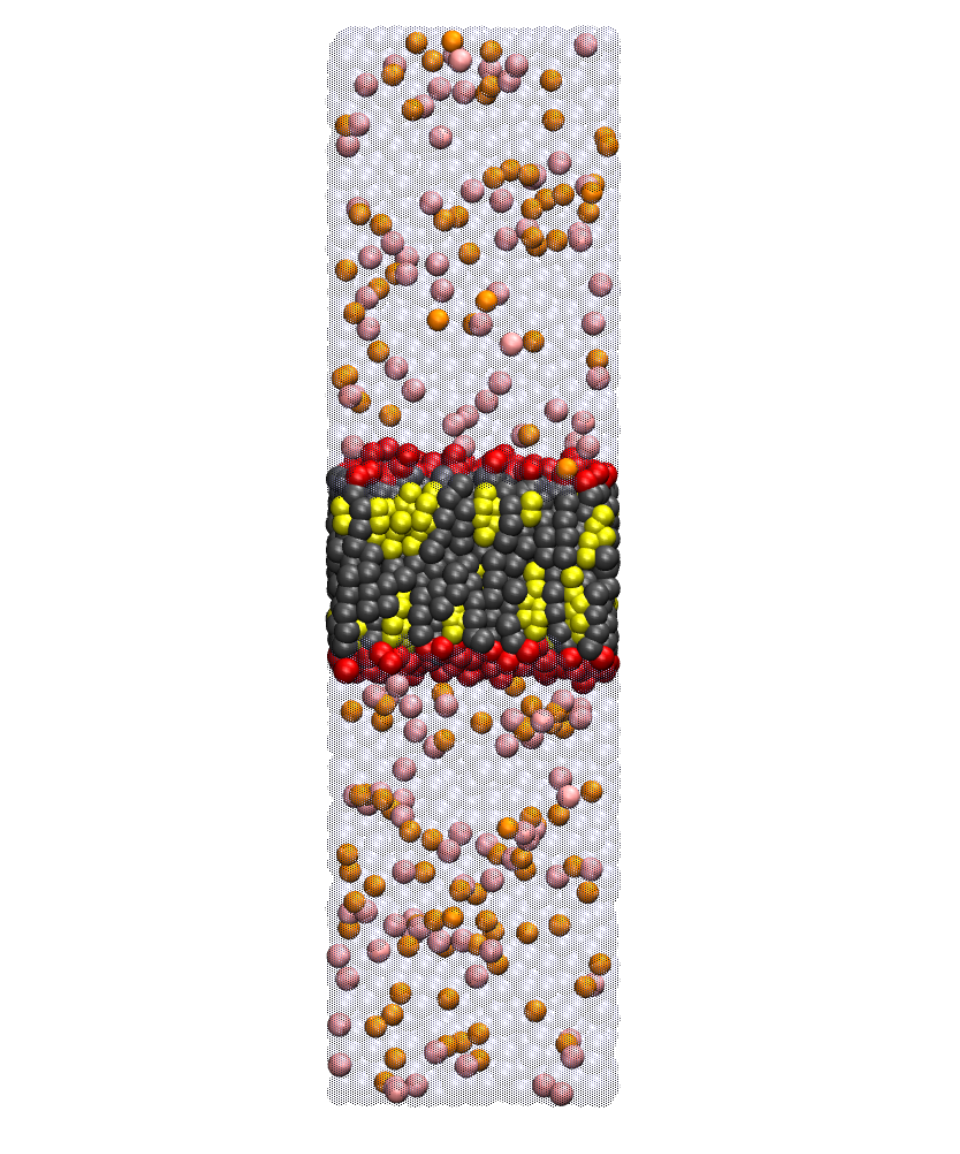
\includegraphics[width=\textwidth]{imagens/dspc_lat.png}
        \caption{DSPC (C18) - Vista Lateral}
    \end{subfigure}

    \vspace{0.5cm} 

    % ================= LINHA 2: Vistas Isométricas =================
    \begin{subfigure}[b]{0.26\textwidth}
        \centering
        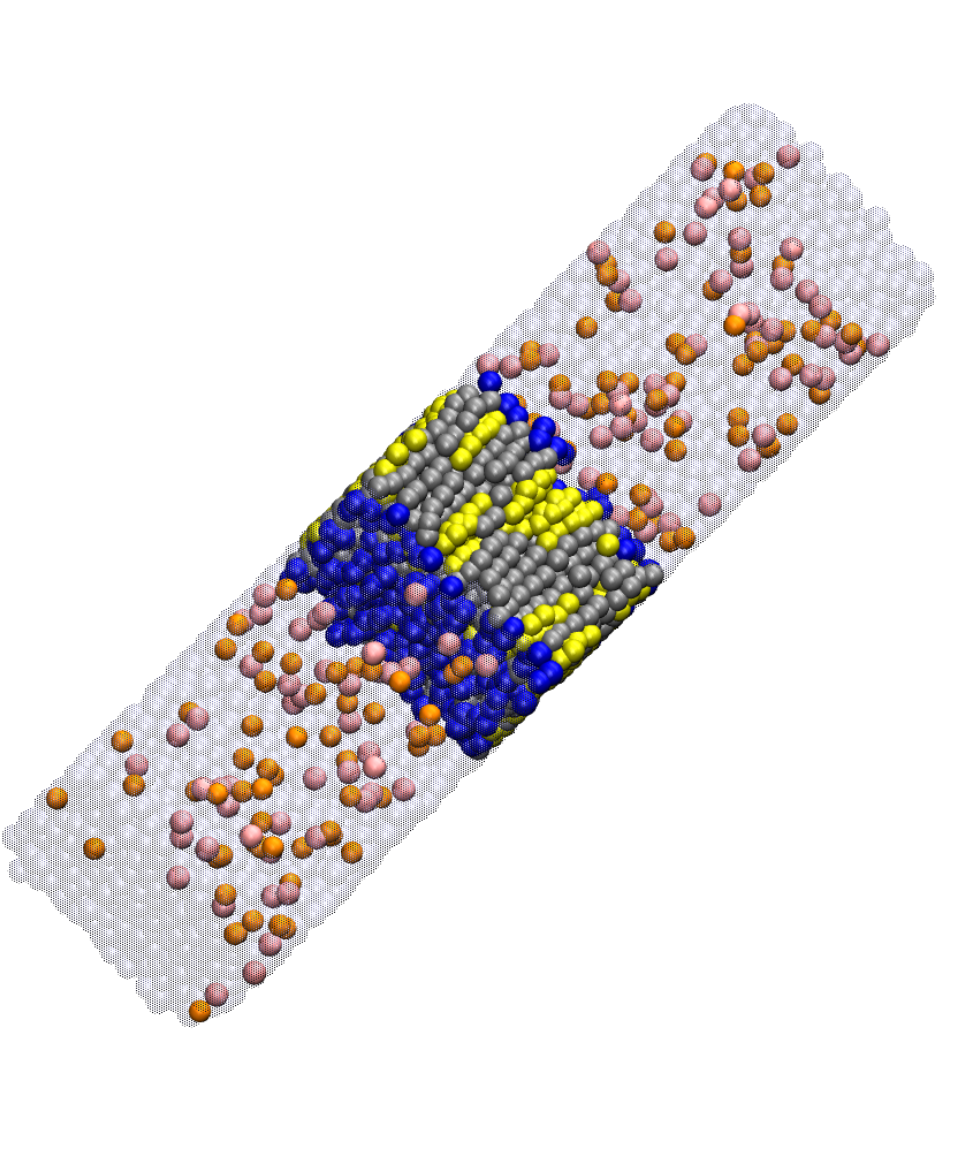
\includegraphics[width=\textwidth]{imagens/dppc_iso.png}
        \caption{DPPC (C16) - Perspectiva}
    \end{subfigure}
    \hspace{1.5cm} 
    \begin{subfigure}[b]{0.26\textwidth}
        \centering
        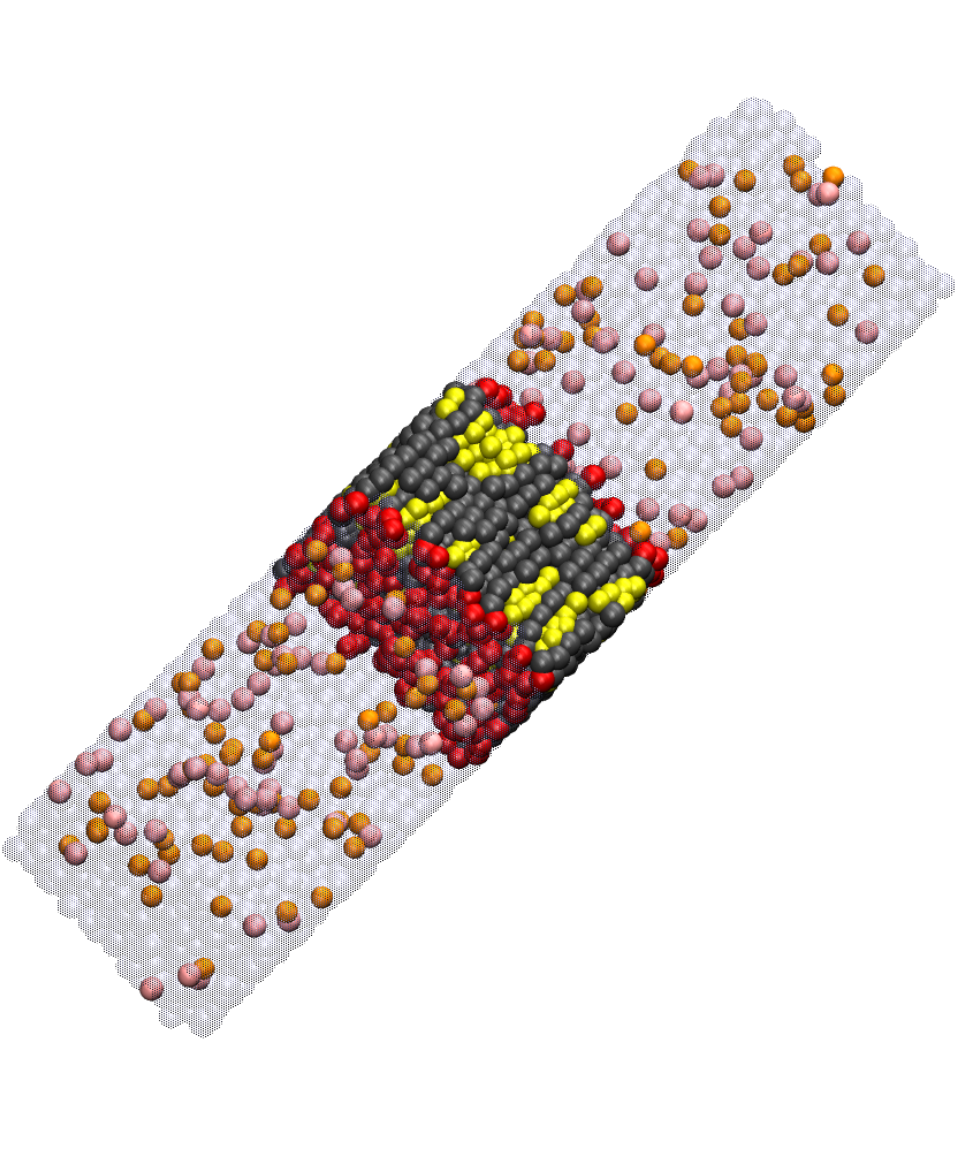
\includegraphics[width=\textwidth]{imagens/dspc_iso.png}
        \caption{DSPC (C18) - Perspectiva}
    \end{subfigure}

    \caption{Comparativo visual do efeito do comprimento da cadeia acílica (\textit{mismatch} hidrofóbico) na estrutura da bicamada a 310 K. À esquerda, o sistema composto por DPPC (16 carbonos) apresenta um núcleo hidrofóbico mais estreito. À direita, o sistema composto por DSPC (18 carbonos) evidencia um ganho de espessura na membrana e uma alteração na distribuição geométrica da solvatação.}
    \label{fig:mosaico_mismatch}
\end{figure}


\bibliographystyle{unsrtnat} 
\bibliography{referencias}

\newpage % Opcional, para garantir que o anexo comece em uma página nova
\section{Tabela Completa de Energias por Réplica e Temperatura}
\label{anexo:tabela_energias_completa}

A tabela a seguir documenta os valores exatos de energia eletrostática (Coulomb) e força de dispersão (Lennard-Jones), juntamente com seus respectivos desvios padrões, para cada simulação individual (todas as proporções molares e temperaturas termotrópicas estudadas).

\footnotesize
\begin{longtable}{|c|c|c|c|c|c|}
\caption{Dados brutos completos de energias de Coulomb e Lennard-Jones.} \label{tab:dados_brutos_energias} \\
\toprule
\textbf{Sistema} & \textbf{Prop.} & \textbf{Temp.} & \textbf{C (kJ/mol)} & \textbf{LJ (kJ/mol)} & \textbf{Total (kJ/mol)} \\ \midrule
\endfirsthead

\multicolumn{5}{c}%
{{\bfseries \tablename\ \thetable{} -- continuação da página anterior}} \\
\toprule
\textbf{Sistema} & \textbf{Prop.} & \textbf{Temp.} & \textbf{C (kJ/mol)} & \textbf{LJ (kJ/mol)} & \textbf{Total (kJ/mol)} \\ \midrule
\endhead

\midrule
\multicolumn{5}{r}{{Continua na próxima página...}} \\
\endfoot

\bottomrule
\endlastfoot

\midrule \multicolumn{5}{c}{\textbf{15W\_L (15 W/L)}} \\ \midrule
15W\_L & 0:100 & 290K & $-792.5 \pm 34.7$ & $-60504.2 \pm 286.0$ & $-61296.7 \pm 288.1$ \\
15W\_L & 0:100 & 300K & $-786.8 \pm 33.6$ & $-59493.6 \pm 339.5$ & $-60280.4 \pm 341.2$ \\
15W\_L & 0:100 & 310K & $-775.6 \pm 38.1$ & $-58655.8 \pm 348.3$ & $-59431.4 \pm 350.4$ \\
15W\_L & 0:100 & 320K & $-766.2 \pm 34.3$ & $-57755.2 \pm 358.7$ & $-58521.4 \pm 360.3$ \\
15W\_L & 0:100 & 333K & $-672.1 \pm 39.7$ & $-51767.5 \pm 420.4$ & $-52439.6 \pm 422.3$ \\
15W\_L & 0:100 & 340K & $-648.9 \pm 39.2$ & $-50771.8 \pm 412.9$ & $-51420.7 \pm 414.8$ \\
15W\_L & 0:100 & 350K & $-621.8 \pm 37.3$ & $-49411.5 \pm 441.8$ & $-50033.3 \pm 443.4$ \\
15W\_L & 100:0 & 290K & $-806.8 \pm 35.4$ & $-57613.2 \pm 286.5$ & $-58420.0 \pm 288.7$ \\
15W\_L & 100:0 & 300K & $-791.8 \pm 37.3$ & $-56953.5 \pm 305.2$ & $-57745.3 \pm 307.5$ \\
15W\_L & 100:0 & 310K & $-784.0 \pm 37.2$ & $-56450.1 \pm 316.8$ & $-57234.1 \pm 319.0$ \\
15W\_L & 100:0 & 320K & $-690.0 \pm 39.9$ & $-51367.3 \pm 392.6$ & $-52057.3 \pm 394.6$ \\
15W\_L & 100:0 & 333K & $-650.6 \pm 37.7$ & $-49757.1 \pm 368.8$ & $-50407.7 \pm 370.7$ \\
15W\_L & 100:0 & 340K & $-634.5 \pm 39.0$ & $-48962.4 \pm 397.0$ & $-49596.9 \pm 398.9$ \\
15W\_L & 100:0 & 350K & $-612.1 \pm 36.5$ & $-47854.1 \pm 403.5$ & $-48466.2 \pm 405.1$ \\
15W\_L & 25:75 & 290K & $-799.1 \pm 36.8$ & $-59810.7 \pm 307.0$ & $-60609.8 \pm 309.2$ \\
15W\_L & 25:75 & 300K & $-790.5 \pm 36.7$ & $-58420.4 \pm 318.9$ & $-59210.9 \pm 321.0$ \\
15W\_L & 25:75 & 310K & $-784.8 \pm 39.3$ & $-58141.7 \pm 297.3$ & $-58926.5 \pm 299.9$ \\
15W\_L & 25:75 & 320K & $-750.4 \pm 37.4$ & $-57006.7 \pm 341.4$ & $-57757.1 \pm 343.4$ \\
15W\_L & 25:75 & 333K & $-668.8 \pm 37.4$ & $-51418.8 \pm 422.9$ & $-52087.6 \pm 424.6$ \\
15W\_L & 25:75 & 340K & $-647.5 \pm 37.2$ & $-50393.7 \pm 405.5$ & $-51041.2 \pm 407.2$ \\
15W\_L & 25:75 & 350K & $-623.3 \pm 38.1$ & $-49114.8 \pm 413.5$ & $-49738.1 \pm 415.3$ \\
15W\_L & 50:50 & 290K & $-804.9 \pm 34.4$ & $-59344.3 \pm 296.4$ & $-60149.2 \pm 298.4$ \\
15W\_L & 50:50 & 300K & $-789.9 \pm 36.8$ & $-57927.9 \pm 305.6$ & $-58717.8 \pm 307.8$ \\
15W\_L & 50:50 & 310K & $-775.9 \pm 38.8$ & $-57633.8 \pm 320.2$ & $-58409.7 \pm 322.5$ \\
15W\_L & 50:50 & 320K & $-746.5 \pm 37.4$ & $-55308.9 \pm 350.7$ & $-56055.4 \pm 352.7$ \\
15W\_L & 50:50 & 333K & $-659.7 \pm 38.2$ & $-51005.9 \pm 391.2$ & $-51665.6 \pm 393.1$ \\
15W\_L & 50:50 & 340K & $-642.8 \pm 40.5$ & $-50067.3 \pm 385.9$ & $-50710.1 \pm 388.0$ \\
15W\_L & 50:50 & 350K & $-615.5 \pm 35.6$ & $-48889.8 \pm 392.2$ & $-49505.3 \pm 393.8$ \\
15W\_L & 75:25 & 290K & $-805.8 \pm 36.8$ & $-57932.1 \pm 274.3$ & $-58737.9 \pm 276.8$ \\
15W\_L & 75:25 & 300K & $-791.2 \pm 36.8$ & $-56874.2 \pm 324.8$ & $-57665.4 \pm 326.9$ \\
15W\_L & 75:25 & 310K & $-776.0 \pm 37.5$ & $-56727.1 \pm 309.9$ & $-57503.1 \pm 312.2$ \\
15W\_L & 75:25 & 320K & $-723.8 \pm 46.7$ & $-53654.8 \pm 1862.1$ & $-54378.6 \pm 1862.7$ \\
15W\_L & 75:25 & 333K & $-658.8 \pm 37.4$ & $-50272.4 \pm 398.9$ & $-50931.2 \pm 400.6$ \\
15W\_L & 75:25 & 340K & $-641.7 \pm 38.4$ & $-49399.1 \pm 386.6$ & $-50040.8 \pm 388.5$ \\
15W\_L & 75:25 & 350K & $-619.3 \pm 39.1$ & $-48262.3 \pm 374.6$ & $-48881.6 \pm 376.6$ \\
\midrule \multicolumn{5}{c}{\textbf{27W\_L (27 W/L)}} \\ \midrule
27W\_L & 0:100 & 290K & $-647.3 \pm 34.1$ & $-195333.6 \pm 457.7$ & $-195980.9 \pm 459.0$ \\
27W\_L & 0:100 & 300K & $-640.5 \pm 35.1$ & $-193439.3 \pm 469.4$ & $-194079.8 \pm 470.7$ \\
27W\_L & 0:100 & 310K & $-626.1 \pm 35.8$ & $-191225.4 \pm 482.7$ & $-191851.5 \pm 484.0$ \\
27W\_L & 0:100 & 320K & $-750.0 \pm 38.7$ & $-171994.7 \pm 504.0$ & $-172744.7 \pm 505.5$ \\
27W\_L & 0:100 & 333K & $-658.9 \pm 38.0$ & $-163911.6 \pm 605.8$ & $-164570.5 \pm 607.0$ \\
27W\_L & 0:100 & 340K & $-634.4 \pm 39.9$ & $-161704.4 \pm 645.3$ & $-162338.8 \pm 646.5$ \\
27W\_L & 0:100 & 350K & $-593.7 \pm 39.3$ & $-158722.0 \pm 663.0$ & $-159315.7 \pm 664.2$ \\
27W\_L & 100:0 & 290K & $-798.6 \pm 36.7$ & $-177183.6 \pm 480.3$ & $-177982.2 \pm 481.7$ \\
27W\_L & 100:0 & 300K & $-784.5 \pm 36.7$ & $-175287.1 \pm 480.1$ & $-176071.6 \pm 481.5$ \\
27W\_L & 100:0 & 310K & $-762.2 \pm 35.7$ & $-172113.4 \pm 554.7$ & $-172875.6 \pm 555.8$ \\
27W\_L & 100:0 & 320K & $-685.3 \pm 39.4$ & $-166705.1 \pm 606.1$ & $-167390.4 \pm 607.4$ \\
27W\_L & 100:0 & 333K & $-628.8 \pm 38.0$ & $-162578.6 \pm 630.6$ & $-163207.4 \pm 631.7$ \\
27W\_L & 100:0 & 340K & $-618.1 \pm 38.6$ & $-160998.4 \pm 602.3$ & $-161616.5 \pm 603.5$ \\
27W\_L & 100:0 & 350K & $-583.6 \pm 38.9$ & $-157904.7 \pm 596.6$ & $-158488.3 \pm 597.9$ \\
27W\_L & 25:75 & 290K & $-651.6 \pm 35.7$ & $-194559.6 \pm 465.6$ & $-195211.2 \pm 467.0$ \\
27W\_L & 25:75 & 300K & $-623.4 \pm 36.6$ & $-192989.5 \pm 468.2$ & $-193612.9 \pm 469.6$ \\
27W\_L & 25:75 & 310K & $-778.1 \pm 37.4$ & $-173646.0 \pm 512.9$ & $-174424.1 \pm 514.3$ \\
27W\_L & 25:75 & 320K & $-762.7 \pm 38.0$ & $-171447.3 \pm 598.8$ & $-172210.0 \pm 600.0$ \\
27W\_L & 25:75 & 333K & $-656.6 \pm 38.9$ & $-163193.4 \pm 633.7$ & $-163850.0 \pm 634.9$ \\
27W\_L & 25:75 & 340K & $-630.7 \pm 37.3$ & $-161146.6 \pm 601.4$ & $-161777.3 \pm 602.6$ \\
27W\_L & 25:75 & 350K & $-596.0 \pm 36.4$ & $-158148.3 \pm 643.9$ & $-158744.3 \pm 644.9$ \\
27W\_L & 50:50 & 290K & $-642.5 \pm 34.2$ & $-193203.4 \pm 431.9$ & $-193845.9 \pm 433.3$ \\
27W\_L & 50:50 & 300K & $-645.9 \pm 34.6$ & $-192228.2 \pm 463.7$ & $-192874.1 \pm 465.0$ \\
27W\_L & 50:50 & 310K & $-623.1 \pm 37.4$ & $-188888.7 \pm 500.4$ & $-189511.8 \pm 501.8$ \\
27W\_L & 50:50 & 320K & $-751.8 \pm 38.7$ & $-169594.8 \pm 697.5$ & $-170346.6 \pm 698.6$ \\
27W\_L & 50:50 & 333K & $-652.6 \pm 38.8$ & $-162576.7 \pm 582.2$ & $-163229.3 \pm 583.5$ \\
27W\_L & 50:50 & 340K & $-631.5 \pm 34.2$ & $-160523.7 \pm 605.7$ & $-161155.2 \pm 606.7$ \\
27W\_L & 50:50 & 350K & $-595.9 \pm 38.2$ & $-157670.9 \pm 599.1$ & $-158266.8 \pm 600.3$ \\
27W\_L & 75:25 & 290K & $-652.1 \pm 33.9$ & $-193974.4 \pm 448.9$ & $-194626.5 \pm 450.2$ \\
27W\_L & 75:25 & 300K & $-633.0 \pm 34.6$ & $-191933.2 \pm 444.0$ & $-192566.2 \pm 445.3$ \\
27W\_L & 75:25 & 310K & $-620.6 \pm 35.7$ & $-189931.6 \pm 477.1$ & $-190552.2 \pm 478.4$ \\
27W\_L & 75:25 & 320K & $-692.4 \pm 35.2$ & $-166114.9 \pm 571.5$ & $-166807.3 \pm 572.6$ \\
27W\_L & 75:25 & 333K & $-646.5 \pm 37.8$ & $-162184.1 \pm 597.0$ & $-162830.6 \pm 598.2$ \\
27W\_L & 75:25 & 340K & $-622.1 \pm 36.6$ & $-160195.5 \pm 597.6$ & $-160817.6 \pm 598.7$ \\
27W\_L & 75:25 & 350K & $-594.1 \pm 39.5$ & $-157429.7 \pm 599.8$ & $-158023.8 \pm 601.1$ \\
\midrule \multicolumn{5}{c}{\textbf{45W\_L (45 W/L)}} \\ \midrule
45W\_L & 0:100 & 290K & $-650.5 \pm 35.9$ & $-296434.9 \pm 498.1$ & $-297085.4 \pm 499.4$ \\
45W\_L & 0:100 & 300K & $-637.5 \pm 35.8$ & $-293974.4 \pm 573.8$ & $-294611.9 \pm 574.9$ \\
45W\_L & 0:100 & 310K & $-775.7 \pm 38.3$ & $-258594.3 \pm 627.8$ & $-259370.0 \pm 629.0$ \\
45W\_L & 0:100 & 320K & $-756.5 \pm 38.8$ & $-254606.2 \pm 693.2$ & $-255362.7 \pm 694.3$ \\
45W\_L & 0:100 & 333K & $-661.8 \pm 37.3$ & $-245387.6 \pm 740.5$ & $-246049.4 \pm 741.4$ \\
45W\_L & 0:100 & 340K & $-634.6 \pm 37.7$ & $-242389.5 \pm 754.8$ & $-243024.1 \pm 755.7$ \\
45W\_L & 0:100 & 350K & $-601.1 \pm 41.0$ & $-238170.1 \pm 713.9$ & $-238771.2 \pm 715.1$ \\
45W\_L & 100:0 & 290K & $-798.7 \pm 32.9$ & $-262677.3 \pm 599.4$ & $-263476.0 \pm 600.3$ \\
45W\_L & 100:0 & 300K & $-779.0 \pm 38.3$ & $-259036.7 \pm 590.1$ & $-259815.7 \pm 591.3$ \\
45W\_L & 100:0 & 310K & $-776.3 \pm 38.8$ & $-256247.6 \pm 641.8$ & $-257023.9 \pm 643.0$ \\
45W\_L & 100:0 & 320K & $-678.6 \pm 39.6$ & $-248486.0 \pm 680.0$ & $-249164.6 \pm 681.2$ \\
45W\_L & 100:0 & 333K & $-635.2 \pm 38.8$ & $-243268.8 \pm 670.4$ & $-243904.0 \pm 671.5$ \\
45W\_L & 100:0 & 340K & $-620.0 \pm 37.8$ & $-240593.6 \pm 741.2$ & $-241213.6 \pm 742.2$ \\
45W\_L & 100:0 & 350K & $-588.5 \pm 33.6$ & $-236555.4 \pm 751.7$ & $-237143.9 \pm 752.5$ \\
45W\_L & 25:75 & 290K & $-659.1 \pm 34.0$ & $-293458.2 \pm 509.3$ & $-294117.3 \pm 510.4$ \\
45W\_L & 25:75 & 300K & $-792.4 \pm 34.3$ & $-260939.6 \pm 654.2$ & $-261732.0 \pm 655.1$ \\
45W\_L & 25:75 & 310K & $-772.8 \pm 36.9$ & $-257370.3 \pm 633.0$ & $-258143.1 \pm 634.1$ \\
45W\_L & 25:75 & 320K & $-761.9 \pm 40.1$ & $-254318.6 \pm 648.8$ & $-255080.5 \pm 650.0$ \\
45W\_L & 25:75 & 333K & $-657.3 \pm 35.4$ & $-244876.3 \pm 754.3$ & $-245533.6 \pm 755.1$ \\
45W\_L & 25:75 & 340K & $-631.8 \pm 37.8$ & $-241950.9 \pm 706.5$ & $-242582.7 \pm 707.5$ \\
45W\_L & 25:75 & 350K & $-596.0 \pm 36.5$ & $-237801.5 \pm 731.3$ & $-238397.5 \pm 732.2$ \\
45W\_L & 50:50 & 290K & $-814.8 \pm 36.0$ & $-264597.3 \pm 589.8$ & $-265412.1 \pm 590.9$ \\
45W\_L & 50:50 & 300K & $-781.7 \pm 36.4$ & $-260935.9 \pm 639.1$ & $-261717.6 \pm 640.1$ \\
45W\_L & 50:50 & 310K & $-771.9 \pm 36.9$ & $-256711.8 \pm 650.2$ & $-257483.7 \pm 651.2$ \\
45W\_L & 50:50 & 320K & $-746.3 \pm 38.6$ & $-252661.6 \pm 1120.7$ & $-253407.9 \pm 1121.4$ \\
45W\_L & 50:50 & 333K & $-652.8 \pm 39.1$ & $-244355.1 \pm 696.9$ & $-245007.9 \pm 698.0$ \\
45W\_L & 50:50 & 340K & $-630.1 \pm 38.8$ & $-241524.5 \pm 710.4$ & $-242154.6 \pm 711.5$ \\
45W\_L & 50:50 & 350K & $-595.5 \pm 38.6$ & $-237446.2 \pm 782.4$ & $-238041.7 \pm 783.4$ \\
45W\_L & 75:25 & 290K & $-800.4 \pm 36.5$ & $-264932.3 \pm 593.1$ & $-265732.7 \pm 594.2$ \\
45W\_L & 75:25 & 300K & $-795.6 \pm 35.7$ & $-261611.3 \pm 620.0$ & $-262406.9 \pm 621.0$ \\
45W\_L & 75:25 & 310K & $-770.5 \pm 35.7$ & $-257993.8 \pm 629.6$ & $-258764.3 \pm 630.6$ \\
45W\_L & 75:25 & 320K & $-756.6 \pm 36.1$ & $-254158.4 \pm 650.3$ & $-254915.0 \pm 651.3$ \\
45W\_L & 75:25 & 333K & $-657.9 \pm 39.2$ & $-244838.8 \pm 697.7$ & $-245496.7 \pm 698.8$ \\
45W\_L & 75:25 & 340K & $-630.9 \pm 37.4$ & $-241864.6 \pm 720.7$ & $-242495.5 \pm 721.7$ \\
45W\_L & 75:25 & 350K & $-598.5 \pm 38.3$ & $-237852.4 \pm 744.2$ & $-238450.9 \pm 745.2$ \\
\midrule \multicolumn{5}{c}{\textbf{CHOL\_0}} \\ \midrule
CHOL\_0 & 0:100 & 290K & $-968.8 \pm 37.7$ & $-291576.6 \pm 612.0$ & $-292545.4 \pm 613.2$ \\
CHOL\_0 & 0:100 & 300K & $-962.4 \pm 40.3$ & $-287532.9 \pm 623.9$ & $-288495.3 \pm 625.2$ \\
CHOL\_0 & 0:100 & 310K & $-943.5 \pm 39.9$ & $-283690.6 \pm 732.7$ & $-284634.1 \pm 733.8$ \\
CHOL\_0 & 0:100 & 320K & $-921.2 \pm 41.3$ & $-279793.0 \pm 711.1$ & $-280714.2 \pm 712.3$ \\
CHOL\_0 & 0:100 & 333K & $-803.7 \pm 44.3$ & $-268481.2 \pm 796.5$ & $-269284.9 \pm 797.7$ \\
CHOL\_0 & 0:100 & 340K & $-767.6 \pm 42.0$ & $-265037.2 \pm 746.5$ & $-265804.8 \pm 747.7$ \\
CHOL\_0 & 0:100 & 350K & $-722.7 \pm 39.2$ & $-260395.1 \pm 804.4$ & $-261117.8 \pm 805.4$ \\
CHOL\_0 & 100:0 & 290K & $-972.1 \pm 41.5$ & $-287749.3 \pm 617.9$ & $-288721.4 \pm 619.3$ \\
CHOL\_0 & 100:0 & 300K & $-951.5 \pm 38.0$ & $-283591.4 \pm 624.9$ & $-284542.9 \pm 626.1$ \\
CHOL\_0 & 100:0 & 310K & $-932.5 \pm 41.6$ & $-279737.9 \pm 679.3$ & $-280670.4 \pm 680.6$ \\
CHOL\_0 & 100:0 & 320K & $-827.7 \pm 41.5$ & $-271786.0 \pm 694.2$ & $-272613.7 \pm 695.4$ \\
CHOL\_0 & 100:0 & 333K & $-771.9 \pm 43.2$ & $-265983.9 \pm 715.6$ & $-266755.8 \pm 716.9$ \\
CHOL\_0 & 100:0 & 340K & $-746.1 \pm 43.4$ & $-262862.2 \pm 777.8$ & $-263608.3 \pm 779.0$ \\
CHOL\_0 & 100:0 & 350K & $-716.1 \pm 42.5$ & $-258646.9 \pm 747.5$ & $-259363.0 \pm 748.7$ \\
CHOL\_0 & 25:75 & 290K & $-973.1 \pm 41.4$ & $-290253.4 \pm 645.9$ & $-291226.5 \pm 647.2$ \\
CHOL\_0 & 25:75 & 300K & $-948.5 \pm 41.4$ & $-286517.2 \pm 670.6$ & $-287465.7 \pm 671.9$ \\
CHOL\_0 & 25:75 & 310K & $-932.7 \pm 38.2$ & $-281893.8 \pm 655.0$ & $-282826.5 \pm 656.1$ \\
CHOL\_0 & 25:75 & 320K & $-909.6 \pm 43.0$ & $-278759.4 \pm 666.5$ & $-279669.0 \pm 667.9$ \\
CHOL\_0 & 25:75 & 333K & $-795.2 \pm 44.2$ & $-267896.5 \pm 816.8$ & $-268691.7 \pm 818.0$ \\
CHOL\_0 & 25:75 & 340K & $-763.1 \pm 44.4$ & $-264608.0 \pm 730.6$ & $-265371.1 \pm 731.9$ \\
CHOL\_0 & 25:75 & 350K & $-719.4 \pm 43.8$ & $-259947.9 \pm 794.8$ & $-260667.3 \pm 796.0$ \\
CHOL\_0 & 50:50 & 290K & $-975.2 \pm 41.9$ & $-289419.8 \pm 610.7$ & $-290395.0 \pm 612.1$ \\
CHOL\_0 & 50:50 & 300K & $-957.5 \pm 39.9$ & $-285116.0 \pm 631.1$ & $-286073.5 \pm 632.4$ \\
CHOL\_0 & 50:50 & 310K & $-935.3 \pm 41.4$ & $-281152.0 \pm 703.6$ & $-282087.3 \pm 704.8$ \\
CHOL\_0 & 50:50 & 320K & $-915.9 \pm 42.0$ & $-277776.0 \pm 855.9$ & $-278691.9 \pm 856.9$ \\
CHOL\_0 & 50:50 & 333K & $-784.8 \pm 43.8$ & $-267345.9 \pm 814.2$ & $-268130.7 \pm 815.4$ \\
CHOL\_0 & 50:50 & 340K & $-756.4 \pm 46.1$ & $-264005.6 \pm 720.4$ & $-264762.0 \pm 721.9$ \\
CHOL\_0 & 50:50 & 350K & $-722.6 \pm 42.2$ & $-259667.6 \pm 754.8$ & $-260390.2 \pm 756.0$ \\
CHOL\_0 & 75:25 & 290K & $-974.3 \pm 41.4$ & $-289042.2 \pm 608.3$ & $-290016.5 \pm 609.7$ \\
CHOL\_0 & 75:25 & 300K & $-951.3 \pm 41.4$ & $-284355.0 \pm 636.3$ & $-285306.3 \pm 637.6$ \\
CHOL\_0 & 75:25 & 310K & $-929.4 \pm 41.6$ & $-280610.6 \pm 631.7$ & $-281540.0 \pm 633.1$ \\
CHOL\_0 & 75:25 & 320K & $-840.1 \pm 43.8$ & $-272681.6 \pm 767.4$ & $-273521.7 \pm 768.6$ \\
CHOL\_0 & 75:25 & 333K & $-780.4 \pm 42.6$ & $-266578.6 \pm 730.7$ & $-267359.0 \pm 731.9$ \\
CHOL\_0 & 75:25 & 340K & $-752.7 \pm 42.7$ & $-263413.3 \pm 778.4$ & $-264166.0 \pm 779.6$ \\
CHOL\_0 & 75:25 & 350K & $-714.1 \pm 41.4$ & $-259107.8 \pm 755.6$ & $-259821.9 \pm 756.7$ \\
\midrule \multicolumn{5}{c}{\textbf{CHOL\_0\_salt}} \\ \midrule
CHOL\_0\_salt & 0:100 & 290K & $-2863.4 \pm 64.2$ & $-308162.2 \pm 607.8$ & $-311025.6 \pm 611.2$ \\
CHOL\_0\_salt & 0:100 & 300K & $-2821.8 \pm 65.2$ & $-305181.5 \pm 608.3$ & $-308003.3 \pm 611.8$ \\
CHOL\_0\_salt & 0:100 & 310K & $-2807.3 \pm 68.1$ & $-301292.6 \pm 653.2$ & $-304099.9 \pm 656.7$ \\
CHOL\_0\_salt & 0:100 & 320K & $-2770.7 \pm 69.8$ & $-297304.0 \pm 685.4$ & $-300074.7 \pm 688.9$ \\
CHOL\_0\_salt & 0:100 & 333K & $-2662.2 \pm 64.0$ & $-286194.6 \pm 784.9$ & $-288856.8 \pm 787.5$ \\
CHOL\_0\_salt & 0:100 & 340K & $-2625.8 \pm 65.9$ & $-282952.7 \pm 809.2$ & $-285578.5 \pm 811.9$ \\
CHOL\_0\_salt & 0:100 & 350K & $-2584.2 \pm 66.2$ & $-278299.1 \pm 825.4$ & $-280883.3 \pm 828.1$ \\
CHOL\_0\_salt & 100:0 & 290K & $-2857.7 \pm 65.9$ & $-305737.7 \pm 624.4$ & $-308595.4 \pm 627.9$ \\
CHOL\_0\_salt & 100:0 & 300K & $-2826.9 \pm 65.5$ & $-301872.9 \pm 603.6$ & $-304699.8 \pm 607.1$ \\
CHOL\_0\_salt & 100:0 & 310K & $-2791.1 \pm 66.3$ & $-298117.7 \pm 709.2$ & $-300908.8 \pm 712.3$ \\
CHOL\_0\_salt & 100:0 & 320K & $-2700.0 \pm 62.2$ & $-289451.3 \pm 711.9$ & $-292151.3 \pm 714.6$ \\
CHOL\_0\_salt & 100:0 & 333K & $-2637.3 \pm 62.5$ & $-283780.4 \pm 714.2$ & $-286417.7 \pm 716.9$ \\
CHOL\_0\_salt & 100:0 & 340K & $-2607.8 \pm 65.1$ & $-280763.8 \pm 748.4$ & $-283371.6 \pm 751.2$ \\
CHOL\_0\_salt & 100:0 & 350K & $-2576.7 \pm 66.4$ & $-276463.8 \pm 725.5$ & $-279040.5 \pm 728.5$ \\
CHOL\_0\_salt & 25:75 & 290K & $-2854.0 \pm 64.1$ & $-305042.7 \pm 589.2$ & $-307896.7 \pm 592.7$ \\
CHOL\_0\_salt & 25:75 & 300K & $-2828.9 \pm 66.1$ & $-301915.7 \pm 641.6$ & $-304744.6 \pm 645.0$ \\
CHOL\_0\_salt & 25:75 & 310K & $-2803.7 \pm 68.3$ & $-297444.9 \pm 641.4$ & $-300248.6 \pm 645.0$ \\
CHOL\_0\_salt & 25:75 & 320K & $-2770.6 \pm 69.7$ & $-293370.1 \pm 673.7$ & $-296140.7 \pm 677.3$ \\
CHOL\_0\_salt & 25:75 & 333K & $-2660.4 \pm 66.2$ & $-283487.3 \pm 753.6$ & $-286147.7 \pm 756.5$ \\
CHOL\_0\_salt & 25:75 & 340K & $-2622.1 \pm 64.9$ & $-280242.9 \pm 775.4$ & $-282865.0 \pm 778.1$ \\
CHOL\_0\_salt & 25:75 & 350K & $-2580.7 \pm 66.2$ & $-275698.2 \pm 815.8$ & $-278278.9 \pm 818.5$ \\
CHOL\_0\_salt & 50:50 & 290K & $-2845.5 \pm 65.6$ & $-304383.3 \pm 645.4$ & $-307228.8 \pm 648.7$ \\
CHOL\_0\_salt & 50:50 & 300K & $-2821.7 \pm 67.3$ & $-301108.9 \pm 745.9$ & $-303930.6 \pm 748.9$ \\
CHOL\_0\_salt & 50:50 & 310K & $-2790.4 \pm 64.2$ & $-296560.5 \pm 647.1$ & $-299350.9 \pm 650.3$ \\
CHOL\_0\_salt & 50:50 & 320K & $-2767.1 \pm 67.1$ & $-292717.1 \pm 713.2$ & $-295484.2 \pm 716.3$ \\
CHOL\_0\_salt & 50:50 & 333K & $-2652.5 \pm 62.3$ & $-282862.9 \pm 751.3$ & $-285515.4 \pm 753.9$ \\
CHOL\_0\_salt & 50:50 & 340K & $-2609.9 \pm 68.8$ & $-279686.6 \pm 774.5$ & $-282296.5 \pm 777.5$ \\
CHOL\_0\_salt & 50:50 & 350K & $-2572.3 \pm 65.9$ & $-275266.6 \pm 760.2$ & $-277838.9 \pm 763.1$ \\
CHOL\_0\_salt & 75:25 & 290K & $-2858.6 \pm 66.0$ & $-303644.5 \pm 620.2$ & $-306503.1 \pm 623.7$ \\
CHOL\_0\_salt & 75:25 & 300K & $-2821.0 \pm 61.8$ & $-300150.4 \pm 653.4$ & $-302971.4 \pm 656.3$ \\
CHOL\_0\_salt & 75:25 & 310K & $-2795.5 \pm 69.4$ & $-296087.7 \pm 671.3$ & $-298883.2 \pm 674.9$ \\
CHOL\_0\_salt & 75:25 & 320K & $-2699.4 \pm 69.0$ & $-288080.4 \pm 711.7$ & $-290779.8 \pm 715.0$ \\
CHOL\_0\_salt & 75:25 & 333K & $-2640.7 \pm 65.1$ & $-282203.4 \pm 715.1$ & $-284844.1 \pm 718.1$ \\
CHOL\_0\_salt & 75:25 & 340K & $-2601.9 \pm 64.0$ & $-279072.2 \pm 771.8$ & $-281674.1 \pm 774.4$ \\
CHOL\_0\_salt & 75:25 & 350K & $-2574.2 \pm 64.6$ & $-274792.8 \pm 732.9$ & $-277367.0 \pm 735.7$ \\
\midrule \multicolumn{5}{c}{\textbf{CHOL\_3}} \\ \midrule
CHOL\_3 & 0:100 & 290K & $-918.1 \pm 39.6$ & $-292315.0 \pm 577.9$ & $-293233.1 \pm 579.3$ \\
CHOL\_3 & 0:100 & 300K & $-899.8 \pm 38.1$ & $-288894.6 \pm 608.1$ & $-289794.4 \pm 609.3$ \\
CHOL\_3 & 0:100 & 310K & $-884.3 \pm 38.9$ & $-284792.8 \pm 666.8$ & $-285677.1 \pm 667.9$ \\
CHOL\_3 & 0:100 & 320K & $-857.8 \pm 37.3$ & $-280977.4 \pm 651.6$ & $-281835.2 \pm 652.7$ \\
CHOL\_3 & 0:100 & 333K & $-766.4 \pm 39.9$ & $-272891.5 \pm 727.1$ & $-273657.9 \pm 728.2$ \\
CHOL\_3 & 0:100 & 340K & $-734.9 \pm 39.8$ & $-269878.3 \pm 741.0$ & $-270613.2 \pm 742.1$ \\
CHOL\_3 & 0:100 & 350K & $-691.2 \pm 41.6$ & $-265731.5 \pm 751.2$ & $-266422.7 \pm 752.4$ \\
CHOL\_3 & 100:0 & 290K & $-916.9 \pm 39.0$ & $-289616.0 \pm 591.2$ & $-290532.9 \pm 592.5$ \\
CHOL\_3 & 100:0 & 300K & $-900.5 \pm 40.7$ & $-286599.5 \pm 576.0$ & $-287500.0 \pm 577.4$ \\
CHOL\_3 & 100:0 & 310K & $-880.8 \pm 40.4$ & $-282535.6 \pm 637.6$ & $-283416.4 \pm 638.9$ \\
CHOL\_3 & 100:0 & 320K & $-787.2 \pm 39.6$ & $-276015.6 \pm 705.1$ & $-276802.8 \pm 706.2$ \\
CHOL\_3 & 100:0 & 333K & $-738.7 \pm 39.8$ & $-270797.2 \pm 702.5$ & $-271535.9 \pm 703.6$ \\
CHOL\_3 & 100:0 & 340K & $-710.6 \pm 43.1$ & $-267981.2 \pm 663.5$ & $-268691.8 \pm 664.9$ \\
CHOL\_3 & 100:0 & 350K & $-681.8 \pm 43.4$ & $-263991.3 \pm 710.0$ & $-264673.1 \pm 711.3$ \\
CHOL\_3 & 25:75 & 290K & $-917.8 \pm 38.2$ & $-292355.7 \pm 606.2$ & $-293273.5 \pm 607.4$ \\
CHOL\_3 & 25:75 & 300K & $-895.2 \pm 39.2$ & $-287935.9 \pm 575.2$ & $-288831.1 \pm 576.5$ \\
CHOL\_3 & 25:75 & 310K & $-888.2 \pm 38.1$ & $-284712.9 \pm 620.5$ & $-285601.1 \pm 621.7$ \\
CHOL\_3 & 25:75 & 320K & $-859.9 \pm 41.3$ & $-280367.2 \pm 669.3$ & $-281227.1 \pm 670.6$ \\
CHOL\_3 & 25:75 & 333K & $-759.2 \pm 40.0$ & $-272412.2 \pm 716.7$ & $-273171.4 \pm 717.8$ \\
CHOL\_3 & 25:75 & 340K & $-729.2 \pm 38.8$ & $-269447.7 \pm 736.6$ & $-270176.9 \pm 737.6$ \\
CHOL\_3 & 25:75 & 350K & $-690.5 \pm 43.1$ & $-265320.6 \pm 751.1$ & $-266011.1 \pm 752.3$ \\
CHOL\_3 & 50:50 & 290K & $-913.9 \pm 40.1$ & $-291453.8 \pm 560.1$ & $-292367.7 \pm 561.5$ \\
CHOL\_3 & 50:50 & 300K & $-896.8 \pm 40.1$ & $-287813.0 \pm 627.3$ & $-288709.8 \pm 628.6$ \\
CHOL\_3 & 50:50 & 310K & $-891.3 \pm 39.4$ & $-283744.0 \pm 642.6$ & $-284635.3 \pm 643.8$ \\
CHOL\_3 & 50:50 & 320K & $-870.5 \pm 39.8$ & $-280540.1 \pm 647.0$ & $-281410.6 \pm 648.2$ \\
CHOL\_3 & 50:50 & 333K & $-759.8 \pm 41.2$ & $-271966.5 \pm 667.5$ & $-272726.3 \pm 668.8$ \\
CHOL\_3 & 50:50 & 340K & $-726.9 \pm 41.7$ & $-269022.7 \pm 696.5$ & $-269749.6 \pm 697.7$ \\
CHOL\_3 & 50:50 & 350K & $-688.7 \pm 38.1$ & $-264943.0 \pm 738.3$ & $-265631.7 \pm 739.3$ \\
CHOL\_3 & 75:25 & 290K & $-922.8 \pm 40.2$ & $-290728.6 \pm 589.2$ & $-291651.4 \pm 590.6$ \\
CHOL\_3 & 75:25 & 300K & $-904.0 \pm 42.4$ & $-287379.6 \pm 631.5$ & $-288283.6 \pm 632.9$ \\
CHOL\_3 & 75:25 & 310K & $-880.2 \pm 41.2$ & $-283086.7 \pm 622.0$ & $-283966.9 \pm 623.4$ \\
CHOL\_3 & 75:25 & 320K & $-800.3 \pm 41.9$ & $-276733.3 \pm 636.4$ & $-277533.6 \pm 637.8$ \\
CHOL\_3 & 75:25 & 333K & $-743.0 \pm 41.2$ & $-271328.7 \pm 674.8$ & $-272071.7 \pm 676.1$ \\
CHOL\_3 & 75:25 & 340K & $-715.7 \pm 43.3$ & $-268494.0 \pm 718.0$ & $-269209.7 \pm 719.3$ \\
CHOL\_3 & 75:25 & 350K & $-682.0 \pm 43.2$ & $-264512.6 \pm 750.4$ & $-265194.6 \pm 751.6$ \\
\midrule \multicolumn{5}{c}{\textbf{CHOL\_30}} \\ \midrule
CHOL\_30 & 0:100 & 290K & $-591.6 \pm 33.4$ & $-284390.9 \pm 602.5$ & $-284982.5 \pm 603.4$ \\
CHOL\_30 & 0:100 & 300K & $-579.2 \pm 32.3$ & $-280697.7 \pm 600.3$ & $-281276.9 \pm 601.2$ \\
CHOL\_30 & 0:100 & 310K & $-565.7 \pm 33.2$ & $-276863.7 \pm 623.7$ & $-277429.4 \pm 624.6$ \\
CHOL\_30 & 0:100 & 320K & $-544.3 \pm 33.3$ & $-272868.7 \pm 606.2$ & $-273413.0 \pm 607.1$ \\
CHOL\_30 & 0:100 & 333K & $-520.1 \pm 33.0$ & $-267778.3 \pm 696.2$ & $-268298.4 \pm 697.0$ \\
CHOL\_30 & 0:100 & 340K & $-507.0 \pm 32.2$ & $-265051.0 \pm 731.0$ & $-265558.0 \pm 731.7$ \\
CHOL\_30 & 0:100 & 350K & $-487.2 \pm 33.1$ & $-261000.9 \pm 744.6$ & $-261488.1 \pm 745.3$ \\
CHOL\_30 & 100:0 & 290K & $-599.7 \pm 33.4$ & $-282915.9 \pm 581.7$ & $-283515.6 \pm 582.7$ \\
CHOL\_30 & 100:0 & 300K & $-583.4 \pm 33.3$ & $-279190.9 \pm 607.9$ & $-279774.3 \pm 608.8$ \\
CHOL\_30 & 100:0 & 310K & $-567.8 \pm 35.3$ & $-275335.1 \pm 586.4$ & $-275902.9 \pm 587.5$ \\
CHOL\_30 & 100:0 & 320K & $-549.1 \pm 33.6$ & $-271553.9 \pm 656.2$ & $-272103.0 \pm 657.1$ \\
CHOL\_30 & 100:0 & 333K & $-519.6 \pm 35.2$ & $-266418.6 \pm 687.1$ & $-266938.2 \pm 688.0$ \\
CHOL\_30 & 100:0 & 340K & $-507.2 \pm 32.9$ & $-263714.1 \pm 695.3$ & $-264221.3 \pm 696.1$ \\
CHOL\_30 & 100:0 & 350K & $-486.1 \pm 36.1$ & $-259763.4 \pm 679.5$ & $-260249.5 \pm 680.5$ \\
CHOL\_30 & 25:75 & 290K & $-601.2 \pm 31.8$ & $-284300.4 \pm 585.5$ & $-284901.6 \pm 586.4$ \\
CHOL\_30 & 25:75 & 300K & $-587.1 \pm 31.8$ & $-280483.0 \pm 612.0$ & $-281070.1 \pm 612.8$ \\
CHOL\_30 & 25:75 & 310K & $-565.2 \pm 33.1$ & $-276395.5 \pm 648.9$ & $-276960.7 \pm 649.7$ \\
CHOL\_30 & 25:75 & 320K & $-543.9 \pm 34.4$ & $-272642.5 \pm 673.1$ & $-273186.4 \pm 674.0$ \\
CHOL\_30 & 25:75 & 333K & $-523.0 \pm 31.6$ & $-267516.7 \pm 695.0$ & $-268039.7 \pm 695.7$ \\
CHOL\_30 & 25:75 & 340K & $-512.4 \pm 32.4$ & $-264849.1 \pm 688.1$ & $-265361.5 \pm 688.9$ \\
CHOL\_30 & 25:75 & 350K & $-484.0 \pm 35.8$ & $-260816.1 \pm 736.4$ & $-261300.1 \pm 737.3$ \\
CHOL\_30 & 50:50 & 290K & $-600.4 \pm 32.7$ & $-283824.1 \pm 575.4$ & $-284424.5 \pm 576.3$ \\
CHOL\_30 & 50:50 & 300K & $-584.5 \pm 33.5$ & $-280008.6 \pm 615.9$ & $-280593.1 \pm 616.8$ \\
CHOL\_30 & 50:50 & 310K & $-566.2 \pm 32.8$ & $-276171.7 \pm 592.6$ & $-276737.9 \pm 593.5$ \\
CHOL\_30 & 50:50 & 320K & $-547.2 \pm 32.6$ & $-272369.5 \pm 666.2$ & $-272916.7 \pm 667.0$ \\
CHOL\_30 & 50:50 & 333K & $-524.2 \pm 33.6$ & $-267211.4 \pm 676.1$ & $-267735.6 \pm 676.9$ \\
CHOL\_30 & 50:50 & 340K & $-504.2 \pm 33.1$ & $-264488.1 \pm 730.5$ & $-264992.3 \pm 731.2$ \\
CHOL\_30 & 50:50 & 350K & $-485.6 \pm 32.7$ & $-260539.9 \pm 714.8$ & $-261025.5 \pm 715.5$ \\
CHOL\_30 & 75:25 & 290K & $-604.5 \pm 31.6$ & $-283393.4 \pm 585.9$ & $-283997.9 \pm 586.8$ \\
CHOL\_30 & 75:25 & 300K & $-589.2 \pm 30.4$ & $-279780.6 \pm 572.7$ & $-280369.8 \pm 573.5$ \\
CHOL\_30 & 75:25 & 310K & $-568.7 \pm 32.0$ & $-275809.9 \pm 624.8$ & $-276378.6 \pm 625.6$ \\
CHOL\_30 & 75:25 & 320K & $-547.8 \pm 32.0$ & $-271964.2 \pm 655.4$ & $-272512.0 \pm 656.2$ \\
CHOL\_30 & 75:25 & 333K & $-523.4 \pm 33.8$ & $-266950.3 \pm 676.5$ & $-267473.7 \pm 677.3$ \\
CHOL\_30 & 75:25 & 340K & $-512.9 \pm 32.9$ & $-264165.9 \pm 656.1$ & $-264678.8 \pm 656.9$ \\
CHOL\_30 & 75:25 & 350K & $-485.4 \pm 33.3$ & $-260196.9 \pm 745.6$ & $-260682.3 \pm 746.3$ \\
\midrule \multicolumn{5}{c}{\textbf{CHOL\_40\_salt}} \\ \midrule
CHOL\_40\_salt & 0:100 & 290K & $-2398.2 \pm 59.5$ & $-297704.2 \pm 559.3$ & $-300102.4 \pm 562.5$ \\
CHOL\_40\_salt & 0:100 & 300K & $-2379.5 \pm 57.1$ & $-294042.2 \pm 592.8$ & $-296421.7 \pm 595.5$ \\
CHOL\_40\_salt & 0:100 & 310K & $-2354.7 \pm 58.3$ & $-290378.3 \pm 640.9$ & $-292733.0 \pm 643.5$ \\
CHOL\_40\_salt & 0:100 & 320K & $-2338.1 \pm 59.4$ & $-286687.1 \pm 680.3$ & $-289025.2 \pm 682.9$ \\
CHOL\_40\_salt & 0:100 & 333K & $-2315.8 \pm 59.9$ & $-281895.5 \pm 667.9$ & $-284211.3 \pm 670.6$ \\
CHOL\_40\_salt & 0:100 & 340K & $-2298.0 \pm 57.8$ & $-279242.3 \pm 709.3$ & $-281540.3 \pm 711.7$ \\
CHOL\_40\_salt & 0:100 & 350K & $-2279.5 \pm 61.5$ & $-275425.9 \pm 737.3$ & $-277705.4 \pm 739.9$ \\
CHOL\_40\_salt & 100:0 & 290K & $-2410.4 \pm 59.1$ & $-296579.2 \pm 584.8$ & $-298989.6 \pm 587.8$ \\
CHOL\_40\_salt & 100:0 & 300K & $-2393.1 \pm 55.9$ & $-293016.0 \pm 576.9$ & $-295409.1 \pm 579.6$ \\
CHOL\_40\_salt & 100:0 & 310K & $-2369.7 \pm 56.9$ & $-289336.7 \pm 618.3$ & $-291706.4 \pm 620.9$ \\
CHOL\_40\_salt & 100:0 & 320K & $-2344.4 \pm 59.1$ & $-285597.0 \pm 646.9$ & $-287941.4 \pm 649.6$ \\
CHOL\_40\_salt & 100:0 & 333K & $-2322.3 \pm 58.9$ & $-280796.5 \pm 687.1$ & $-283118.8 \pm 689.6$ \\
CHOL\_40\_salt & 100:0 & 340K & $-2301.0 \pm 60.3$ & $-278204.7 \pm 681.5$ & $-280505.7 \pm 684.2$ \\
CHOL\_40\_salt & 100:0 & 350K & $-2285.4 \pm 60.6$ & $-274357.7 \pm 713.2$ & $-276643.1 \pm 715.8$ \\
CHOL\_40\_salt & 25:75 & 290K & $-2401.7 \pm 62.7$ & $-297470.6 \pm 592.5$ & $-299872.3 \pm 595.8$ \\
CHOL\_40\_salt & 25:75 & 300K & $-2383.0 \pm 61.6$ & $-293824.2 \pm 614.5$ & $-296207.2 \pm 617.6$ \\
CHOL\_40\_salt & 25:75 & 310K & $-2366.8 \pm 62.9$ & $-290255.7 \pm 618.2$ & $-292622.5 \pm 621.4$ \\
CHOL\_40\_salt & 25:75 & 320K & $-2347.1 \pm 62.9$ & $-286541.4 \pm 652.6$ & $-288888.5 \pm 655.6$ \\
CHOL\_40\_salt & 25:75 & 333K & $-2317.5 \pm 59.4$ & $-281691.2 \pm 660.0$ & $-284008.7 \pm 662.7$ \\
CHOL\_40\_salt & 25:75 & 340K & $-2300.9 \pm 58.4$ & $-279034.0 \pm 697.9$ & $-281334.9 \pm 700.3$ \\
CHOL\_40\_salt & 25:75 & 350K & $-2281.7 \pm 59.2$ & $-275237.0 \pm 772.8$ & $-277518.7 \pm 775.1$ \\
CHOL\_40\_salt & 50:50 & 290K & $-2408.3 \pm 60.9$ & $-297255.3 \pm 581.7$ & $-299663.6 \pm 584.9$ \\
CHOL\_40\_salt & 50:50 & 300K & $-2388.4 \pm 60.9$ & $-293605.7 \pm 578.8$ & $-295994.1 \pm 582.0$ \\
CHOL\_40\_salt & 50:50 & 310K & $-2365.4 \pm 58.6$ & $-289971.2 \pm 591.6$ & $-292336.6 \pm 594.5$ \\
CHOL\_40\_salt & 50:50 & 320K & $-2349.6 \pm 61.8$ & $-286286.6 \pm 636.6$ & $-288636.2 \pm 639.6$ \\
CHOL\_40\_salt & 50:50 & 333K & $-2316.4 \pm 58.9$ & $-281414.1 \pm 725.9$ & $-283730.5 \pm 728.3$ \\
CHOL\_40\_salt & 50:50 & 340K & $-2301.2 \pm 60.9$ & $-278835.3 \pm 673.4$ & $-281136.5 \pm 676.1$ \\
CHOL\_40\_salt & 50:50 & 350K & $-2280.8 \pm 59.7$ & $-274980.1 \pm 715.7$ & $-277260.9 \pm 718.2$ \\
CHOL\_40\_salt & 75:25 & 290K & $-2406.6 \pm 63.3$ & $-296894.3 \pm 571.0$ & $-299300.9 \pm 574.5$ \\
CHOL\_40\_salt & 75:25 & 300K & $-2392.0 \pm 59.0$ & $-293390.8 \pm 633.2$ & $-295782.8 \pm 635.9$ \\
CHOL\_40\_salt & 75:25 & 310K & $-2375.8 \pm 59.3$ & $-289683.7 \pm 616.8$ & $-292059.5 \pm 619.6$ \\
CHOL\_40\_salt & 75:25 & 320K & $-2345.0 \pm 58.2$ & $-285917.6 \pm 628.0$ & $-288262.6 \pm 630.7$ \\
CHOL\_40\_salt & 75:25 & 333K & $-2314.9 \pm 58.9$ & $-281182.0 \pm 687.8$ & $-283496.9 \pm 690.3$ \\
CHOL\_40\_salt & 75:25 & 340K & $-2305.5 \pm 62.9$ & $-278541.2 \pm 730.8$ & $-280846.7 \pm 733.5$ \\
CHOL\_40\_salt & 75:25 & 350K & $-2283.7 \pm 57.2$ & $-274727.3 \pm 701.3$ & $-277011.0 \pm 703.6$ \\
\midrule \multicolumn{5}{c}{\textbf{CHOL\_4\_salt}} \\ \midrule
CHOL\_4\_salt & 0:100 & 290K & $-2801.6 \pm 66.2$ & $-308242.6 \pm 586.3$ & $-311044.2 \pm 590.0$ \\
CHOL\_4\_salt & 0:100 & 300K & $-2760.4 \pm 64.8$ & $-304733.0 \pm 600.8$ & $-307493.4 \pm 604.3$ \\
CHOL\_4\_salt & 0:100 & 310K & $-2748.8 \pm 66.2$ & $-301297.9 \pm 622.8$ & $-304046.7 \pm 626.3$ \\
CHOL\_4\_salt & 0:100 & 320K & $-2723.6 \pm 61.2$ & $-297562.6 \pm 666.1$ & $-300286.2 \pm 668.9$ \\
CHOL\_4\_salt & 0:100 & 333K & $-2624.7 \pm 66.5$ & $-288855.4 \pm 709.5$ & $-291480.1 \pm 712.6$ \\
CHOL\_4\_salt & 0:100 & 340K & $-2591.4 \pm 66.3$ & $-285851.6 \pm 737.1$ & $-288443.0 \pm 740.1$ \\
CHOL\_4\_salt & 0:100 & 350K & $-2543.3 \pm 65.4$ & $-281613.9 \pm 717.3$ & $-284157.2 \pm 720.3$ \\
CHOL\_4\_salt & 100:0 & 290K & $-2795.3 \pm 64.6$ & $-305843.4 \pm 612.3$ & $-308638.7 \pm 615.7$ \\
CHOL\_4\_salt & 100:0 & 300K & $-2777.7 \pm 67.4$ & $-301806.4 \pm 595.6$ & $-304584.1 \pm 599.4$ \\
CHOL\_4\_salt & 100:0 & 310K & $-2750.3 \pm 62.6$ & $-298733.7 \pm 628.9$ & $-301484.0 \pm 632.0$ \\
CHOL\_4\_salt & 100:0 & 320K & $-2663.7 \pm 66.1$ & $-291983.5 \pm 610.3$ & $-294647.2 \pm 613.9$ \\
CHOL\_4\_salt & 100:0 & 333K & $-2604.3 \pm 68.7$ & $-286716.0 \pm 700.8$ & $-289320.3 \pm 704.2$ \\
CHOL\_4\_salt & 100:0 & 340K & $-2574.6 \pm 64.3$ & $-283887.0 \pm 714.4$ & $-286461.6 \pm 717.3$ \\
CHOL\_4\_salt & 100:0 & 350K & $-2541.7 \pm 68.2$ & $-280023.5 \pm 728.8$ & $-282565.2 \pm 732.0$ \\
CHOL\_4\_salt & 25:75 & 290K & $-2790.9 \pm 68.1$ & $-307918.6 \pm 606.5$ & $-310709.5 \pm 610.3$ \\
CHOL\_4\_salt & 25:75 & 300K & $-2766.9 \pm 65.0$ & $-304093.3 \pm 640.8$ & $-306860.2 \pm 644.1$ \\
CHOL\_4\_salt & 25:75 & 310K & $-2760.6 \pm 63.4$ & $-300105.1 \pm 609.8$ & $-302865.7 \pm 613.1$ \\
CHOL\_4\_salt & 25:75 & 320K & $-2717.2 \pm 65.0$ & $-296286.4 \pm 645.7$ & $-299003.6 \pm 649.0$ \\
CHOL\_4\_salt & 25:75 & 333K & $-2617.3 \pm 65.1$ & $-288304.1 \pm 677.2$ & $-290921.4 \pm 680.3$ \\
CHOL\_4\_salt & 25:75 & 340K & $-2592.0 \pm 64.8$ & $-285390.9 \pm 741.5$ & $-287982.9 \pm 744.3$ \\
CHOL\_4\_salt & 25:75 & 350K & $-2544.0 \pm 65.1$ & $-281261.7 \pm 734.6$ & $-283805.7 \pm 737.5$ \\
CHOL\_4\_salt & 50:50 & 290K & $-2796.8 \pm 60.0$ & $-307474.7 \pm 569.0$ & $-310271.5 \pm 572.2$ \\
CHOL\_4\_salt & 50:50 & 300K & $-2777.5 \pm 70.4$ & $-303232.6 \pm 635.4$ & $-306010.1 \pm 639.3$ \\
CHOL\_4\_salt & 50:50 & 310K & $-2750.4 \pm 68.6$ & $-299517.9 \pm 658.2$ & $-302268.3 \pm 661.8$ \\
CHOL\_4\_salt & 50:50 & 320K & $-2723.5 \pm 68.1$ & $-295741.8 \pm 607.1$ & $-298465.3 \pm 610.9$ \\
CHOL\_4\_salt & 50:50 & 333K & $-2618.3 \pm 68.7$ & $-287931.6 \pm 697.1$ & $-290549.9 \pm 700.5$ \\
CHOL\_4\_salt & 50:50 & 340K & $-2588.0 \pm 66.7$ & $-284945.6 \pm 710.8$ & $-287533.6 \pm 713.9$ \\
CHOL\_4\_salt & 50:50 & 350K & $-2545.3 \pm 64.6$ & $-280893.6 \pm 746.2$ & $-283438.9 \pm 749.0$ \\
CHOL\_4\_salt & 75:25 & 290K & $-2804.9 \pm 64.5$ & $-306327.2 \pm 595.4$ & $-309132.1 \pm 598.9$ \\
CHOL\_4\_salt & 75:25 & 300K & $-2770.2 \pm 61.7$ & $-302334.1 \pm 597.4$ & $-305104.3 \pm 600.6$ \\
CHOL\_4\_salt & 75:25 & 310K & $-2744.3 \pm 66.0$ & $-298804.6 \pm 611.4$ & $-301548.9 \pm 615.0$ \\
CHOL\_4\_salt & 75:25 & 320K & $-2702.5 \pm 68.2$ & $-294553.5 \pm 1186.7$ & $-297256.0 \pm 1188.7$ \\
CHOL\_4\_salt & 75:25 & 333K & $-2614.4 \pm 66.2$ & $-287321.7 \pm 708.0$ & $-289936.1 \pm 711.1$ \\
CHOL\_4\_salt & 75:25 & 340K & $-2582.0 \pm 63.5$ & $-284443.9 \pm 690.4$ & $-287025.9 \pm 693.3$ \\
CHOL\_4\_salt & 75:25 & 350K & $-2540.0 \pm 66.5$ & $-280429.8 \pm 752.1$ & $-282969.8 \pm 755.0$ \\
\end{longtable}
\normalsize
\normalsize


\end{document}


\section{CONCLUSÃO}

A investigação termodinâmica e estrutural conduzida neste trabalho evidenciou a complexa rede de forças que governa a estabilidade e a dinâmica de fases das membranas lipídicas. Utilizando simulações de Dinâmica Molecular com o campo de força \textit{coarse-grained} Martini 3, foi possível não apenas capturar as propriedades macroscópicas esperadas, mas também dissecar quantitativamente os domínios de energia eletrostática (Coulomb) e de dispersão (Lennard-Jones) subjacentes a esses fenômenos.

A análise sob diferentes gradientes de hidratação revelou uma marcante assimetria cinética entre fosfolipídios homólogos. Demonstrou-se que a matriz de DSPC ($C_{18}$), ao contrário do DPPC ($C_{16}$), sucumbe a uma armadilha metaestável sob alta hidratação, manifestando-se como um líquido super-resfriado. Esta retenção foi termodinamicamente associada à barreira entálpica de dessolvatação interfacial: a alta inércia estérica das cadeias maiores exige uma energia de ativação cooperativa que suplanta as flutuações térmicas disponíveis, impedindo a cristalização espontânea para a fase gel.

A modulação imposta pela inserção de colesterol elucidou o funcionamento de um mecanismo de compensação isoperibólica de extrema elegância biofísica. A drástica condensação lateral induzida pelas altas concentrações de esterol força a expulsão da água interfacial, o que acarreta um severo déficit nas interações de Coulomb e na hidratação primária. Contudo, demonstrou-se que a energia global de dispersão do sistema se mantém estável, pois o custo da dessolvatação é integralmente neutralizado pelo ganho de contatos atrativos de van der Waals decorrentes do empacotamento linear (\textit{all-trans}) das caudas hidrofóbicas contra a estrutura rígida do esterol.

Adicionalmente, a inserção de íons no sistema evidenciou o papel da coordenação do sódio ($Na^+$) na estabilização adicional da interface polar. Contudo, em misturas saturadas com colesterol (40\% em mol), a rigidez mecânica imposta pela fase líquida-ordenada ($L_o$) torna-se dominante, anulando a cooperatividade intrínseca da matriz lipídica e sobrepondo-se até mesmo aos fortes efeitos de ancoragem iônica.

Os resultados aqui consolidados transcendem o entendimento fundamental da física de membranas. Ao comprovar a sensibilidade topológica e a precisão do modelo Martini 3 no balanço de interações não-covalentes, este trabalho pavimenta um alicerce para a biofísica translacional. A elucidação da dinâmica interfacial e do empacotamento lipídico estabelece diretrizes termodinâmicas rigorosas para o \textit{design} de lipossomas na vetorização de fármacos e para a prospecção \textit{in silico} de agentes antivirais, consolidando a Dinâmica Molecular como uma ferramenta preditiva indispensável e de altíssimo rigor para o avanço da física médica.


% --- PÓS-TEXTUAIS ---
\singlespacing
\bibliographystyle{estilo_ufg}
\section{CONCLUSÃO}

A investigação termodinâmica e estrutural conduzida neste trabalho evidenciou a complexa rede de forças que governa a estabilidade e a dinâmica de fases das membranas lipídicas. Utilizando simulações de Dinâmica Molecular com o campo de força \textit{coarse-grained} Martini 3, foi possível não apenas capturar as propriedades macroscópicas esperadas, mas também dissecar quantitativamente os domínios de energia eletrostática (Coulomb) e de dispersão (Lennard-Jones) subjacentes a esses fenômenos.

A análise sob diferentes gradientes de hidratação revelou uma marcante assimetria cinética entre fosfolipídios homólogos. Demonstrou-se que a matriz de DSPC ($C_{18}$), ao contrário do DPPC ($C_{16}$), sucumbe a uma armadilha metaestável sob alta hidratação, manifestando-se como um líquido super-resfriado. Esta retenção foi termodinamicamente associada à barreira entálpica de dessolvatação interfacial: a alta inércia estérica das cadeias maiores exige uma energia de ativação cooperativa que suplanta as flutuações térmicas disponíveis, impedindo a cristalização espontânea para a fase gel.

A modulação imposta pela inserção de colesterol elucidou o funcionamento de um mecanismo de compensação isoperibólica de extrema elegância biofísica. A drástica condensação lateral induzida pelas altas concentrações de esterol força a expulsão da água interfacial, o que acarreta um severo déficit nas interações de Coulomb e na hidratação primária. Contudo, demonstrou-se que a energia global de dispersão do sistema se mantém estável, pois o custo da dessolvatação é integralmente neutralizado pelo ganho de contatos atrativos de van der Waals decorrentes do empacotamento linear (\textit{all-trans}) das caudas hidrofóbicas contra a estrutura rígida do esterol.

Adicionalmente, a inserção de íons no sistema evidenciou o papel da coordenação do sódio ($Na^+$) na estabilização adicional da interface polar. Contudo, em misturas saturadas com colesterol (40\% em mol), a rigidez mecânica imposta pela fase líquida-ordenada ($L_o$) torna-se dominante, anulando a cooperatividade intrínseca da matriz lipídica e sobrepondo-se até mesmo aos fortes efeitos de ancoragem iônica.

Os resultados aqui consolidados transcendem o entendimento fundamental da física de membranas. Ao comprovar a sensibilidade topológica e a precisão do modelo Martini 3 no balanço de interações não-covalentes, este trabalho pavimenta um alicerce para a biofísica translacional. A elucidação da dinâmica interfacial e do empacotamento lipídico estabelece diretrizes termodinâmicas rigorosas para o \textit{design} de lipossomas na vetorização de fármacos e para a prospecção \textit{in silico} de agentes antivirais, consolidando a Dinâmica Molecular como uma ferramenta preditiva indispensável e de altíssimo rigor para o avanço da física médica.


\bibliography{referencias}

\end{document}
